\documentclass[12pt, a4paper]{article}
%\documentclass[12pt, a4paper]{amsart}
\usepackage{amsmath}
\usepackage{amssymb}
\usepackage{amsfonts}
\usepackage{fancyhdr}
\usepackage{dsfont}
\usepackage{graphics}
\usepackage{amscd}
\usepackage{amsthm}
\usepackage{mathrsfs}
\usepackage{enumerate}
\usepackage{mathtools}
\usepackage{booktabs}
\usepackage{array}
\usepackage[pdfborder={0 0 0}]{hyperref}
\usepackage[usenames,dvipsnames]{xcolor}
\usepackage{nth}
\usepackage{float}
\usepackage[T1]{fontenc}
\usepackage{ae,aecompl}
\usepackage{mcode}
\usepackage{color}
\usepackage[normalem]{ulem}
\usepackage{tgpagella}
%TO DO: 
%-Fix bold headings to use \subsection* (??)
%-Insert figures (tikz) (go through notes to check for figures)
%-Put all code using \mcode
%-Fix use of \texttt
%-Add all references (bibtex)
%-Fix use of \vec on vectors and matrices ... :(((

%Some of the computers in the honours room don't have the vector package
%Wavy vectors also breaks a little for subscripts.
%\usepackage[wavy]{vector}
%\renewcommand{\vec}[1]{\uwave{#1}}
\renewcommand{\vec}[1]{\mathbf{#1}}



\def\C{\mathbb{C}}
\def\Q{\mathbb{Q}}
\def\R{\mathbb{R}}
\def\N{\mathbb{N}}
\def\Z{\mathbb{Z}}
\def\T{\mathbb{T}}
\def\hom{\operatorname{Hom}}
\def\id{\operatorname{id}}

\def\sign{\mathop{\mathrm{sign}}}

\newtheorem{thm}{Theorem}[section]
\newtheorem{cor}[thm]{Corollary}
\newtheorem{lemma}[thm]{Lemma}
\newtheorem{prop}[thm]{Proposition}
\newtheorem{thm1}{Theorem}
\newtheorem{definition}[thm]{Definition}
\newtheorem{definitions}[thm]{Definitions}
\theoremstyle{definition}
\newtheorem{example}[thm]{Example}
%\theoremstyle{definition}
\newtheorem{exercise}[thm]{Exercise}
\newtheorem*{aside}{Aside}
\newtheorem*{motivation}{Motivation}
\theoremstyle{remark}
\newtheorem*{remark}{Remark}
\newtheorem{remarks}[thm]{Remarks}
\numberwithin{equation}{section}

% Remove paragraph indent and add spacing
\setlength{\parindent}{0pt}
\setlength{\parskip}{1em}

\newcommand{\HRule}{\rule{\linewidth}{0.5mm}}
\newcommand\bslash{\char`\\}

% Derivative Macros
\newcommand{\dd}[2]{\frac{\textrm{d} #1}{\textrm{d} #2}}
\newcommand{\ddtwo}[2]{\frac{\textrm{d}^{2} #1}{\textrm{d} #2 ^{2}}}
\newcommand{\pdd}[2]{\frac{\partial#1}{\partial#2}}
\newcommand{\pddb}[2]{\left( \frac{\partial#1}{\partial#2} \right)}
\newcommand{\ptwodd}[3]{\frac{\partial^2 #1}{\partial #2\partial #3}}
\newcommand{\ptwoddtwo}[2]{\frac{{\partial}^2 #1}{\partial {#2}^2}}



\renewcommand{\sectionmark}[1]{\markright{#1}{}}
\pagestyle{fancy}
\fancyhead[LO]{Computational Differential Equations}
\fancyhead[CO]{}
\fancyhead[RO]{\rightmark}



\title{MAST90026 Computational Differential Equations Notes}
\date{SM1 2026}
\author{Notes taken in Steven Carnie's 2012 and 2014 Classes\\ 
edited/adapted by James Osborne(2018), Hailong Guo (2020, 2022),\\ Jesse Collis (2024), and Patrick Grant (2026)}

\begin{document}

\maketitle 
\thispagestyle{empty}


\pagenumbering{roman}

\newpage
\setcounter{page}{1}
\section*{Preface}
\addcontentsline{toc}{section}{Preface}
\noindent These notes for the subject MAST90026 Computational Differential Equations were originally produced by a student in the 2012 class, Eddy Qiu. He passed them on to Steven Carnie in December 2013 who turned them into notes for the next class, the class of 2014. Eddy ran out of steam just as time entered the picture. The remaining lectures were transcribed into LaTex  
by Cameron Patrick, Ashley Dyson and Gala Camacho Ferrari of the 2014 class, and James Osborne have used these to make notes for the 2018 class. Hailong Guo modified these notes for the 2020 and 2022 editions of this class, Jesse Collis further modified for the 2024 edition of the class, and I (Patrick Grant) have further refined the class material.

\noindent The notes are inspired by the following works:
\begin{itemize}
\item [-] Ascher, Mattheij \& Russell, Numerical solution of boundary value problems for ordinary differential equations, Prentice-Hall, 1988. 
\item[G] Gockenbach, {\em Understanding and implementing the finite element method}, SIAM, 2006.
\item[I] Iserles, {\em A first course in the numerical analysis of differential equations}, 2nd ed.,  CUP, 2008.
\item [-] Kelley, {\em Iterative Methods for Linear and Nonlinear Equations} , SIAM, 1995.
\item[L] Leveque, {\em Finite Difference Methods for Ordinary and Partial Differential Equations: Steady-State and Time-dependent problems}, SIAM, 2007.
\item [-] Trefethen, Spectral Methods in MATLAB, SIAM, 2000.
\end{itemize}

Patrick Grant

February, 2026
 

\newpage
\tableofcontents



\newpage
\setcounter{page}{1}
\setcounter{section}{-1}
\pagenumbering{arabic}
\section{Introduction}
In this course we aim to cover numerical techniques for solving

\begin{itemize}
\item Boundary value problems (BVPs) for ODEs, (MATLAB commands: \mcode{bvp4c/bvp5c})
\item Simple PDEs
\begin{itemize}
\item 2D Elliptic PDEs
\item 1+1 (1 space dimension, 1 time dimension) Parabolic (MATLAB command: \mcode{pdepe}), Hyperbolic
\end{itemize}
\end{itemize}

For 2D PDEs there is a toolbox in MATLAB \mcode{pdetool}, but there is no toolbox for 3D PDEs!

The sorts of problems we are aiming to deal with include (in decreasing order of difficulty):
\begin{example}[Incompressible Navier-Stokes equations]
\begin{align*}
\vec{u}_t+(\vec{u}\cdot\nabla)\vec{u} &= -\nabla p + \mu\nabla^2\vec{u},\\
\nabla \cdot \vec{u} &= 0.
\end{align*}
\end{example}

\begin{example}[Black-Scholes equation]
\begin{align*}
v_t+\frac{1}{2}\sigma^{2}S^{2}v_{SS}+rSv_{S}-rv=0.
\end{align*}
\end{example}

\newpage

\begin{example}[Convection-diffusion equation]
\begin{align*}
u_t+\vec{v}\cdot\nabla u=\nabla\cdot(\operatorname{D}\nabla u)+f.
\end{align*}

The convection-diffusion equation simplifies in 1D to
\begin{align*}
u_t+v u_x=\operatorname{D}u_{xx}+f.
\end{align*}
\textbf{a)} Letting $v=0$ we get the diffusion/heat equation:
\begin{align*}
u_t=\operatorname{D}u_{xx}+f,
\end{align*}
which is \emph{Parabolic}.

\textbf{b)} Or letting $\operatorname{D}=0$ we get the advection/transport/1-way wave equation.
\begin{align*}
u_t+vu_x=s,
\end{align*}
which we call \emph{Hyperbolic} even though it is first order, because it shares many of the properties of second order Hyperbolic equations.

\textbf{c)}  If we solve for the steady state solution ($u_t=0$) we get:
\begin{equation*}
\vec{v}\cdot\nabla u - \nabla \cdot(\operatorname{D}\nabla u)=f,
\end{equation*}
which is a PDE in space only. 

If $\vec{v}=0$, we get
\begin{equation*}
-\nabla\cdot(\operatorname{D}\nabla u)=f.
\end{equation*}
which is an \emph{Elliptic} PDE. 

\textbf{d)} Finally in one dimension, we get 
\begin{align*}
vu_x -\operatorname{D}u_{xx} =f,
\end{align*}
an ODE with boundary conditions -- a boundary value problem!
\end{example}

\newpage
In discussing numerical methods, we will start with the simplest problems, BVPs, and work our way back up. We probably won't get to 
solving the Navier-Stokes equations, which is typically done with commercial software for Computational Fluid Dynamics (CFD), but I will show you some examples. 
For more details, take ENGR90024 Computational Fluid Dynamics which uses the OpenFoam package. 

We will  concentrate on methods for solving linear BVPs that generalize to solving PDEs and to nonlinear problems.

There are a few general issues we will need to face:
\begin{itemize}
 \item How do we step in time (for IVPs)?
\item How do we we represent the solution in space (for BVPs/PDEs)?
\item How do we handle higher dimensionality?
\item How do we handle non-linearity?
\end{itemize}

\newpage

\subsection{ODE IVP Revision}

Before we look at BVPs we will do a quick Initial Value Problem revision example.

\begin{exercise}
Use MATLAB's inbuilt solvers (or code up your own method) to solve the following system of first order ODE's

\begin{align*}
\dd{S}{t} &= \Pi - \beta S Z - \delta S, \\
\dd{Z}{t} &=  \beta S Z +\zeta R - \alpha S Z, \\
\dd{R}{t} &= \delta S + \alpha S Z- \zeta R, \\
\end{align*}
\end{exercise} 
subject to $S(0)=1000$, $Z(0)=0$, and $R(0)=0$. Where $\Pi=0$, $\beta=0.0095$, $\delta=0.0001$,  $\zeta=0.1$, and $\alpha=0.005$.



\newpage
\section{1D Boundary Value Problems}

First we will look at linear scalar $2^{nd}$ order BVPs.
They are of the form 
\begin{equation*}
u''+p(x)u'+q(x)u=r(x),
\end{equation*}
with \emph{linear separated} boundary conditions at $x=a$ and $x=b$:
\begin{align*}
A_{11}u(a)+A_{12}u'(a)&=\beta_1,\\
A_{21}u(b)+A_{22}u'(b)&=\beta_2.
\end{align*}
These are sometimes called \emph{Robin} boundary conditions.

If $A_{12}=A_{22}=0$:
\begin{align*}
A_{11}u(a)&=\beta_1,\\
A_{21}u(b)&=\beta_2,
\end{align*}
then we get \emph{Dirichlet} boundary conditions.
 Alternatively, if $A_{11}=A_{21}=0$:
\begin{align*}
A_{12}u'(a)&=\beta_1,\\
A_{22}u'(b)&=\beta_2,
\end{align*}
we get \emph{Neumann} boundary conditions.
Note that our BVP may not be nearly as nice as this, both our equation and our boundary conditions could be non-linear.

\newpage
\begin{example}[General scalar $2^{nd}$ order BVPs.] \ \\
They are of the form 
\begin{equation*}
u'' = f(x,u,u'),
\end{equation*}
with \emph{separated} boundary conditions at $x=a$ and $x=b$:
\begin{align*}
g_1(u(a), u'(a))&=B_1,\\
g_2(u(b), u'(b))&=B_2.
\end{align*}
In more generality, we can have BVPs written as first order systems:
\begin{equation*}
{\bf u}' = {\bf f}(x,{\bf u}),
\end{equation*}
with non-separated boundary conditions
\begin{equation*}
{\bf g}({\bf u}(a), {\bf u}(b)) = {\bf 0}.
\end{equation*}
\end{example}


\newpage

There are many methods for solving boundary value problems:
\begin{itemize}
\item \textbf{Shooting:} shooting treats the BVP as a series of initial value problems, then uses the large number of readily available IVP solvers to solve the problem.
\begin{itemize}
\item Simple shooting
\item Multiple shooting
\end{itemize}
\item \textbf{Relaxation:} relaxation reduces the problem into a series of simpler problems.
\begin{itemize}
\item Finite difference methods (FDM): reduce the problem to a set of algebraic equations (linear or non-linear).
\item Weighted residuals: search for a solution in a simpler function space (i.e. the set of piecewise linear functions)
\begin{itemize}
\item Galerkin (finite element methods (FEM))
\item Collocation (pseudospectral)
\end{itemize}
\item Finite volume methods (FVM)
\end{itemize}
\end{itemize}

If we look at the boundary volume problem as
\begin{equation*}
\operatorname{L}u=r(x),
\end{equation*}
then in the FDM we approximate the differential operator $\operatorname{L}$ and in weighted residual methods we approximate the solution $u$. 
In FVM (not covered in this subject), we must have a problem written as a conservation law and approximate the fluxes. 
Note that in 1D, FVM and FDM are the same but in higher dimensions they're not. 

Note that in general it is much harder to guarantee existence or uniqueness of a solution for a BVP as compared to an IVP e.g. for linear BVPs we can get
0, 1 or $\infty$ solutions.

\newpage
\subsection[Finite Difference Methods]{Finite Difference Methods \small {\emph{Leveque, Chapters 1,2}}}
In finite difference methods we aim to approximate $\operatorname{L}=\operatorname{D}^{2} + p(x)\operatorname{D}+q(x)\operatorname{I}$.

\subsubsection{Finite Difference Formulae}

To do this we approximate $u'$ and $u''$ in terms of sampled values of $u(x)$, with each approximation being associated with a
\emph{discretisation error}. For example:
\begin{align*}
u'(x)&=\frac{u(x+h)-u(x)}{h} + \text{error}, &&\mbox{Forward difference formula};\\
u'(x)&=\frac{u(x)-u(x-h)}{h} + \text{error}, &&\mbox{Backward difference formula};\\
u'(x)&=\frac{u(x+h)-u(x-h)}{2h} + \text{error}, &&\mbox{Central difference formula}; and\\
u''(x)&=\frac{u(x+h)-2u(x)+u(x-h)}{h^2} + \text{error}, &&\mbox{Central difference formula}.
\end{align*}

In general we obtain an approximation for $u^{(k)}$:
\begin{equation*}
u^{(k)}(x) =  \sum_{i=1}^n c_i u(x+h_i) +\text{error}.
\end{equation*}
called a \emph{Finite Difference Formula}.

The positions $\{h_i\}$ are determined by the choice of \emph{mesh}, or the values where we are approximating $u$.
The weights $\{c_i \}$ are called the \emph{stencil} and are chosen to achieve a certain error.
$n$ determines how many values we are approximating each point with.

\begin{example}[Forward Difference]\ \\ 
$n=2$, $c_1=-\frac{1}{h}$, $c_2=\frac{1}{h}$ $\rightarrow$ Error = $O(h)$.
\end{example}

\begin{example}[Central Difference (for $u'$)]\ \\
$n=3$, $c_1=-\frac{1}{2h}$, $c_2=0$, $c_3=\frac{1}{2h}$ $\rightarrow$ Error = $O(h^2)$.
\end{example}

If we approximate $u^{(k)}$ with $n$ values our worst-case error is $O(h^{n-k})$, so we would definitely like $n>k$ so that our error
decreases as we decrease the step size!

\subsubsection*{Derivation}

To determine the coefficients (the weights) we fix $\{h_i\}$ and expand $u(x+h_i)$ in Taylor Series. From this we obtain a
system of linear equations for $\{c_i\}$.

Alternatively, it is also possible to use interpolating polynomials. 
If we take the unique interpolating polynomial through $\{(x+h_i,u(x+h_i)\}$, 
differentiate the polynomial and evaluate at each $x+h_i$ we obtain the weights for our approximation.
Leveque provides MATLAB code which generates the required weights (\mcode{fdcoeffF}).

\begin{exercise}
Use the MATLAB function \mcode{fdcoeffF} to calculate the coefficients in the above examples. If you have time, experiment with non uniform meshes. 
\end{exercise}

\newpage
\subsubsection{Discretisation Errors}

To find the errors for our approximations, we use Taylor Series:
\begin{example}[Central Difference Error]
\begin{align*}
&\frac{u(x+h)-u(x-h)}{2h}\\
=&\frac{1}{2h}\left(u(x)+hu'(x)+\frac{1}{2}h^2 u''(x)+O(h^3)\right)-\\
&\frac{1}{2h}\left(u(x)-hu'(x)+\frac{1}{2}h^2 u''(x)+O(h^3)\right)\\
=&\frac{2hu'(x)+O(h^3)}{2h}\\
=&u'(x)+O(h^2),
\end{align*}
\end{example}
where we have assumed that $u$ is sufficiently smooth (e.g.\ for the above example we assumed that $u \in C^3$).

\begin{itemize}
\item The forward difference error is first order.
\item The backward difference error is also first order.
\item As we saw above, the central difference error is second order.
\item The central difference approximation for $u''$ has a second order error if the mesh used is equal spacing, otherwise it is first order in general.
\end{itemize}


\newpage
\begin{exercise}
Use the MATLAB function \mcode{fdstencil} to calculate the dominant terms in the  error for the above examples.  
\end{exercise}

\begin{exercise}
Run the MATLAB script \mcode{chap1example1} to see how the error of a set of approximations to $u'$. Note `Dpu' is the Forward difference formula, `Dmu' is the Backward difference formula, `D0u' is the central difference formula, and  `D3u' is the following approximation
\begin{equation}
D_{3}u(x) = \frac{1}{6h}[2u(x+h) + 3u(x) - 6u(x-h) +u(x-2h)]. \nonumber
\end{equation}  
What is the accuracy of $D_3u$?
\end{exercise}

\subsubsection{Solution off the Mesh}
We end up with a system of linear equations for each of the points on our mesh which we can solve. 
To find the solution off the mesh interpolation is required. The most common form is linear interpolation, but more accurate methods (like splines) could be used, see MAST30028.

\newpage

\subsubsection{A linear BVP with Dirichlet BCs}
We will examine a linear BVP with Dirichlet boundary conditions on a uniform mesh with $N$ internal mesh points.
\begin{align*}
&u''(x)+p(x)u'+q(z)u=r(x),\\
&u(a)=\alpha, u(b)=\beta.
\end{align*}
Let $h=\frac{b-a}{N+1}$, $x_j=a+jh$.
Then, using a central difference approximation for $u'$ and $u''$, at $x_j$:
\begin{equation*}
\frac{u_{j+1}-2u_j+u_{j-1}}{h^2}+p(x_j)\frac{u_{j+1}-u_{j-1}}{2h}+q(x_j)u_j=r(x_j).
\end{equation*}

Letting $p(x_j)=p_j$, $q(x_j)=q_j$ and $r(x_j)=r_j$ we obtain the following system of linear equations:
\begin{align*}
u_0=\alpha,\\
\frac{u_0-2u_1+u_2}{h^2}+p_1\frac{u_2-u_0}{2h}+q_1 u_1=r_1,\\
\frac{u_1-2u_2+u_3}{h^2}+p_2\frac{u_3-u_1}{2h}+q_2 u_2=r_2,\\
\vdots\\
\frac{u_{N-1}-2u_N+u_{N+1}}{h^2}+p_N\frac{u_{N+1}-u_{N-1}}{2h}+q_N u_N=r_N,\\
u_{N+1}=\beta.
\end{align*}

We can eliminate $u_0$ and $u_N+1$ easily,  which would eliminate the first and last equations and change the second and second last equation to:
\begin{align*}
\frac{-2u_1+u_2}{h^2}+p_1\frac{u_2}{2h}+q_1 u_1=r_1-\frac{\alpha}{h^2}+p_1\frac{\alpha}{2h},\\
\frac{u_{N-1}-2u_N}{h^2}+p_N\frac{-u_{N-1}}{2h}+q_N u_N=r_N - \frac{\beta}{h^2}-p_N\frac{\beta}{2h},
\end{align*}
or we could just keep the first and last trivial equations and solve a slightly larger system.

We can write this in matrix form: 
\begin{align*}
\frac{1}{h^2}
&\begin{pmatrix}
-2+h^2q_1 &1+h\frac{p_1}{2}&0 &0\\
1-h\frac{p_2}{2} &\ddots &\ddots &0\\
0 &\ddots &\ddots &1+h\frac{p_{N-1}}{2}\\
0& 0& 1-h\frac{p_N}{2} &-2 +h^2 q_N
\end{pmatrix}
\begin{pmatrix}
u_1\\
u_2\\
\vdots\\
u_N
\end{pmatrix}
\\
=&
\begin{pmatrix}
r_1-\frac{\alpha}{h^2}+p_1\frac{\alpha}{2h}\\
r_2\\
\vdots\\
r_N-\frac{\beta}{h^2}-p_N\frac{\beta}{2h}
\end{pmatrix}
\end{align*}
or ${A} \mathbf{u} = \mathbf{b} $, which can  be be solved using the backslash command in MATLAB (denoted \mcode{\\ } in the text from now on): \mcode{u=A\\b}.

%\newpage


Once we have reduced the problem to a linear system, some obvious questions are:
\begin{enumerate}
\item Does this have a solution?
\item How hard is it to solve?
\item How well does $\bf{u}$ approximate $u(x)$ for a given $h$?
\item Does ${\bf u} \to u(x_j)$ as $h \to 0$?
\end{enumerate}

\newpage
The answers to these questions are:
\begin{enumerate}
\item [1.] A solution exists as long as our matrix is non-singular.  A singular matrix is possible if the underlying boundary value problem has no unique solution,
e.g.  a BVP with Neumann boundary conditions on both sides.

But it can be shown that if the matrix is \emph{strictly diagonal dominant} ($|a_{jj}|>\sum_{i\neq j}|a_{ij}|$), then our matrix will not be  singular (from Linear Algebra). 

For the above matrix this is generally true if $h$ is small and always true if $p=0$ and $q<0$.

\item [2.] A general dense $n \times n$ matrix requires about $\frac{1}{3}n^{3}$ operations to solve (Gaussian elimination with partial pivoting) or more. 

Luckily our matrix is tridiagonal (non zero entries along only the central diagonal and two diagonals above and below it). Without pivoting this takes $5n + 4$ operations and with pivoting it takes $O(n^2)$ operations. It turns out that if a matrix is strictly diagonal dominant, then we can guarantee we will not need pivoting, so our solution will be extremely quick. 

This happy fact is not so true for 2D problems, and will lead us to consider other methods for solving linear systems, iterative methods. 
\item [3/4.] To answer Questions 3 and 4, we need to do some error analysis for BVPs.

\end{enumerate}

\newpage

\subsubsection{Error analysis}

In solving the linear system
\begin{equation*}
A {\mathbf x} = {\bf b},
\end{equation*}
we get the rule of thumb
\begin{equation*}
\mbox{relative forward error} \sim \mbox{condition \#} \times \mbox{relative backward error (residual)}.
\end{equation*}
The condition number is a property of the problem and measures how sensitive the problem output is to a small change in the problem inputs. The backward error is a property of the algorithm and gives how close is the nearby problem it actually solved. As an equation we say
\begin{equation*}
\label{ }
\frac{ \| \mathbf{\Delta x}\|}{\|\mathbf{x}\|} \lesssim \kappa(A)  \left(\frac{\| {\Delta A} \|}{\| { A} \|} + 
\frac{ \|\mathbf{\Delta b}\| }{\| \mathbf{ b} \| }\right),
\end{equation*}
where $\kappa(A)$ is the condition number (for inversion),  the forward error $\mathbf{\Delta x}$ is the error in the solution, and the backward error
${\Delta A}$ (and $\mathbf{\Delta b}$) is the backward error due to the solution algorithm. Notice that here we use vector norms and subordinate matrix norms to measure the errors. 

For initial value problems, we can show (see MAST30028)
\begin{equation*}
\mbox{convergence} \sim \mbox{0-stability} + \mbox{consistency (residual)},
\end{equation*}
where convergence measures the accuracy of our solution, 0-stability measures how much errors of the discrete problem stay bounded as $h \to 0$ (how stable our algorithm is), and consistency relates to how well we approximate the problem (or if we put in the real solution, what kind of residual we obtain).

We aim for a similar result for BVPs, in the form
\begin{equation*}
\mbox{convergence} \sim \mbox{stability} + \mbox{consistency (residual)}.
\end{equation*}

To measure the error we cannot use traditional vector norms because as we refine our mesh our vector grows so even though the accuracy may remain the same or get better the size of our error vector may grow.
Instead we use grid function (i.e. it is only defined on the grid/mesh) norms:
\begin{align*}
\| \Sigma \|_1 &= h \sum|\Sigma_i|,\\
\| \Sigma \|_2 &= \left(h \sum|\Sigma_i|^2 \right)^{\frac{1}{2}},\\
\| \Sigma \|_\infty &= \operatorname{max}|\Sigma_i|. \\
\end{align*}
(Note that the infinity norm for grid functions is the same as the vector infinity norm).
By convergence, we mean the accuracy of the solution or the \emph{global error} which is defined as:
\begin{equation*}
 \| E \| =  \| \mathbf{u} - \mathbf{\hat{u}} \|, 
\end{equation*}
the difference between the computed solution $\mathbf{u} = \{u_j\}$ and the true solution \mbox{$\mathbf{\hat{u}} =\{\hat{u}(x_j)\}$} at the grid points, measured with a grid function norm. 
By residual, we mean the Local Truncation Error. This leads to the following definitions.

\begin{definition}[Convergence] \ \\
A method with global error $\| E\|=O(h^p)$ as $h \to 0$ is convergent of order $p$.
\end{definition} 

%\begin{equation*}
%LTE \times \|A^{-1}\| \ge \| \epsilon \|
%\end{equation*}
%The local truncation error multiplied by the stability bound is greater than or equal to the global error.

\begin{definition}[Local Truncation Error (LTE)] \ \\
The local truncation error $\tau_j$ is the residual at grid point $x_j$ when the true solution is put into the finite difference formula 
\end{definition}

The LTE for our system is given as
\begin{equation*}
\tau_j = \frac{1}{h^2}(u(x_{j+1})-2u(x_j)+u(x_{j-1}))+p(x_j)\frac{u(x_{j+1})-u(x_{j-1})}{2h}+q(x_j)u(x_j)-r(x_j).
\end{equation*}


%$u(x_j) \to f(x_j) = r_j$
%
%Approximate $Lu_{\text{exact}}=f$ by $L_{h}u_{\text{exact}}=f+\tau \implies Au_{\text{exact}}=F+u$ $L_{h}\hat{u}=f \implies Au=f$.

Now to find the size of $\tau_j$ we can use Taylor series (assuming $u \in C^3$) to get the following: 
\begin{align*}
\tau_j&=u''(x_j)+p(x_j)u'(x_j)+q(x_j)u(x_j)-r(x_j)+ C h^2u^{(3)}+O(h^4)\\
&=C h^2u^{(3)}(\xi)+O(h^4),
\end{align*}
so $\tau_j = O(h^2)$.
Define $\tau = (\tau_1, \dots \tau_N)^T$ as a grid function. 

\begin{exercise}
 Using taylor expansion derive the form for $\tau_{j}$ given above.
\end{exercise}

\newpage

\begin{definition}[Consistency]
A method is consistent of order $p$ if \mbox{$\|\tau\| = O(h^p)$} as $h \to 0$.
\end{definition}

\begin{example}
 For the central difference formulae above, $\|\tau\| = O(h^2)$, so the method is consistent of order 2.
\end{example}

For a method to be consistent, it just means you've used a sensible discretisation of the original problem; usually consistency is not an issue. 
We now need to connect the global error and the LTE. 

The exact solution solves the problem 
\[  \operatorname{L} \hat{u} = r(x).\]
By definition of the LTE, it satisfies for the discretized operator $\operatorname{L_h}$ the equation
\[ \operatorname{L_h} \hat{u} = r(x) + \tau, \]
or, when evaluated at the grid points
\[ A  \mathbf{\hat{u}} = \mathbf{b} + \tau. \]
The computed solution satisfies 
\[  A  \mathbf{u} = \mathbf{b}.  \]
so, subtracting we get
\[ A(\mathbf{u} - \mathbf{\hat{u}}) = A E=-\tau,\]
\[ \implies E = -A^{-1}\tau, \] 
where $E$ is the global error, 
so \[\| E \| = \|A^{-1}\tau\| \le \|A^{-1}\|\|\tau\|.\]
This is our connection between the global error and the LTE. 

To make sure the global error becomes small like the LTE, we want $\|A^{-1}\| \le c$ $\forall h \le h_0$.

\begin{definition}[Stability]
A method is stable if $A^{-1}$ exists and \mbox{$\|A^{-1}\| \le c$} $\forall h < h_0$
\end{definition}
Finding such a constant $c$ is called finding a \emph{stability bound}. So a stable discrete matrix stays well-conditioned as $h \to 0$.

\begin{thm}[Convergence]
Consistency + Stability $\implies$ Convergence.

Proof: 
\begin{align*}
&A E= -\tau,\\
\implies & E = -A^{-1}\tau,\\
\implies &\| E\| \le \|A^{-1}\|\|\tau\| \le c C h^{2} = O(h^{2}).
\end{align*}
\end{thm}

Proving stability is often hard  since finding $A^{-1}$ is often harder than solving the problem. Also $A$ increases in size as $h \to 0$. 
\begin{example}
 \emph{Levesque \textsection 2.10, 2.11} proves stablility for $u''=f$ on $[0,1]$ with Dirichlet boundary conditions by proving
\[\|A^{-1}\|_{2} \le \frac{1}{\pi^2}  \quad \text{and} \quad \|A^{-1}\|_{\infty} \le 3. \]
\end{example}

\newpage
%\underline{\bf{Other boundary conditions}}:
\subsubsection{Other boundary conditions}
\begin{itemize}
\item Neumann boundary condition at one boundary, Dirichlet at the other (\emph{mixed boundary conditions})
\item \emph{Robin boundary conditions}: $A_1 u(a) + A_2 u'(a) = B_1$ etc.
\end{itemize}

For these problems we can use:
\begin{itemize}
\item $1^{st}$ Order Method:

We can simply let $u'(x_0)=\alpha \implies \frac{u_1-u_0}{h}=\alpha$ so our error is now $O(h)$ and we have lost $O(h^{2})$ behaviour.

\item $2^{nd}$ Order Methods:
\begin{itemize}
\item Ghost nodes:
\begin{equation*}
\frac{u_{-1}-2u_0+u_1}{h^2}+{p}_0\left(\frac{u_1-u_{-1}}{2h}\right) + q_0 u_0 = r_0,
\end{equation*}
where $u_{-1}$ is a ghost node. Then, to eliminate $u_{-1}$ we apply our boundary conditions, using a central difference to ensure $O(h^2)$:
\begin{align*}
u'(x_0)=\alpha \implies \frac{u_1-u_{-1}}{2h}=\alpha, 
\implies u_{-1} = u_1 -2\alpha h.
\end{align*}

So we obtain for the first row in our matrix:
\begin{equation*}
\frac{-2u_0+2u_1}{h^2} + q_0 u_0 = r_0 - {p}_0\alpha + \frac{2\alpha}{h}.
\end{equation*}

\item Alternatively we can use a 1-sided second order forward difference formula for $u'(x_0)$
\begin{equation*}
u'(x_0) = \frac{-3u_0 + 4u_1 - u_2}{2h}+O(h^2),
\end{equation*}
where we have retained our $O(h^2)$ behaviour. Our first row now has 3 elements instead of 2 so our matrix is no longer tridiagonal, but it is still banded.
\end{itemize}
\end{itemize}

\newpage

\subsection{Method of Weighted Residuals}
We let $u$ be a vector in some function space, called the trial space,  with basis $\{\phi_j\}$ and coefficients $c_j$.
\begin{equation*}
u_N = \sum_{j=0}^N c_j\phi_j.
\end{equation*}

There are then two aspects of our solution where we can make choices.
\begin{enumerate}
\item There are two common ways to choose $\phi_j$:
\begin{itemize}
\item $\phi_j$ are global basis functions. So $\phi_j \neq 0$ over  $[a,b]$ e.g.\ $\sin(jx)$, polynomials.
\item $\phi_j$ are bases of a piecewise polynomial space. So $\phi_j$ has a local support and is only non zero over a compact subset of $[a,b]$ e.g.\ `hat functions' form a basis for piecewise linear functions.
\end{itemize}

\item And then are a few ways to choose a criterion to find our coefficients to minimize the size of the residual $\operatorname{L}u_N-r$.
\begin{itemize}
\item We can force the residual to be equal to 0 at certain $\{x_j\}$ in our domain. This is called \emph{collocation}. 
\item Or we can try and make the residual orthogonal to the function space of our approximate solution $u_N$ (or \emph{trial space}). We call this a \emph{Galerkin} method. This is equivalent to finding a solution in  the trial space that satisfies the \emph{weak form} of the boundary value problem.

\newpage
 \begin{aside}We can also try and make our residual orthogonal to a (different) \emph{test space}. These methods are called \emph{Petrov-Galerkin} methods.
 \end{aside}
  \end{itemize}
\end{enumerate}
These choices give the following methods:
\begin{center}
\begin{tabular}{c|>{\centering}m{4cm}<{\centering}|>{\centering}p{4cm}<{\centering}}
 &Global Basis & Piecewise polynomial / local support \tabularnewline \hline 
 Collocation &\small Spectral Collocation / Pseudospectral & \small Spline Collocation \tabularnewline  \hline
Galerkin & \small Spectral Galerkin & \small Finite Element Methods\tabularnewline 
\end{tabular}
\end{center}

We will not cover Spectral Galerkin methods here.

\newpage
\subsection{Collocation methods}

\subsubsection{Spectral Collocation}
In spectral collocation we first have a trial space:
\begin{enumerate}
\item We can choose a trial space of trigonometric functions:
\begin{equation*}
u_N(x) = \sum_{j=0}^N a_j \cos(jx) + \sum_{j=1}^N b_j\sin(jx) = \sum_{j=-N}^{N} c_j e^{i jx},
\end{equation*}
which is the same as representing our solution by a truncated Fourier series (hence the term \emph{spectral} in spectral collocation).

This choice is good for problems with periodic boundary conditions, e.g.\ $u(0)=u(2\pi)$ (which is not separated), 
since there is a theorem that states we can represent all periodic $L^2$ functions with Fourier series.

\item We can also choose a trial space of polynomials of degree $N$ (order $N+1$).
\begin{equation*}
u_N(x) =p_{N}(x) \in \mathbb{P}_{N+1}.
\end{equation*}
This is more common for non periodic problems on a domain $[a,b]$.

We still have more questions to answer:
\begin{enumerate}
\item What basis functions should we use over the polynomials?
\item What collocation points should we use?
\end{enumerate}

\begin{itemize}
\item We can choose a basis of Legendre polynomials $P_n(x)$ $(n=0,\dots,N)$.

Then choose as collocation points the roots of $P_{N+1}$(\emph{orthogonal collocation}).

\item Or we can first choose to collocate on the \emph{Chebyshev points} (of the second kind): the maxima/minima of $T_N(x)$ (i.e. the Chebyshev polynomial of the first kind)
\begin{equation*}
\{x_k\} = \left\{\cos\left(\frac{\pi k}{N}\right) \bigg| k=0, \dots, N \right\},
\end{equation*}
And then choose the \emph{cardinal basis} (or \emph{nodal basis}) as basis functions:
\begin{equation*}
\ell_j(x_i)=\delta_{ij},
\end{equation*}
i.e.
\begin{equation*}
\ell_j(x)=\prod_{k \neq j} \frac{(x-x_k)}{(x_j-x_k)},
\end{equation*}
which is called the \emph{Lagrange interpolating polynomial.}

With this choice of basis, we have
\begin{equation*}
p_N(x_i) = \sum_{j=0}^{N}u_j\ell_j(x_i) =  c_i,
\end{equation*}
so we can let $c_i=u(x_i)=u_i$ which simplifies things somewhat.
\end{itemize}
\end{enumerate}
\begin{aside}
The polynomial interpolant through $\{x_j,u_j\}$, $(j=0,\dots,N)$ is:
\begin{equation*}
p_N(x) = \sum_{j=0}^{N}u_j\ell_j(x),
\end{equation*}
where $\ell_j(x_i)=\delta_{ij}$ as above.
\end{aside}

\begin{exercise}
Call the function \mcode{rungeinterp}, to see an example of polynomial fitting on equally spaced points, note the Runge Phenomena at the edges.
\end{exercise}

\begin{exercise}
Call the function \mcode{chebRunge}, to see an example of polynomial fitting on Chebyshev points, note the error at the  the edges. 
\end{exercise}

The main advantage of spectral methods is that under the right conditions (i.e.\ $u$ is smooth enough) we can get \emph{spectral convergence}.

i.e.\ $e_N \sim e^{-cN}$ instead of $e_N \sim N^{-p}$ as in FDM and FEM.

So $N$ does not have to be very large for great accuracy. The trade off is that the matrices generated by spectral collocation are dense.

\begin{exercise}
Run the script \mcode{p12} what does this tell you about the error?
\end{exercise}

\begin{example}
Consider the BVP $u''(x)+p(x)u'(x)+q(x)=r(x)$ over $[a,b]$.

First, map the interval $[a,b]$ to $[-1,1]$. $\to u''(t) +\bar{p}(t)u'(t)+\bar{q}u(t)=\bar{r}(t)$.

Let
\begin{equation*}
u_N(x) = \sum_{j=0}^{N}c_j\phi_j(x),
\end{equation*}
and collocate at the Chebyshev points $x_k=\cos(\frac{\pi k}{N})$, $(k=0,\dots,N)$.
Let $\{ \phi_j \} = \mbox{Lagrange polynomials based on the Chebyshev points}$  then, $c_j = u_j$. 
So,
\begin{equation*}
u_N'(x) = \sum_{j=0}^N u_j\phi_j'(x),
\end{equation*}
\begin{equation*}
u_N''(x)  = \sum_{j=0}^{N}u_j\phi_j''(x).
\end{equation*}


Since we are collocating, we only need to find $u'$ and $u''$ at the collocation points.
\begin{align*}
u_N'(x_k) &= \sum_{j=0}^N u_j \phi_j'(x_k) = \sum_{j=0}^N D_{kj}u_j, \quad \text{and} \\
u_N''(x_k) &= \sum_{j=0}^N u_j \phi_j''(x_k) = \sum_{j=0}^N D^{(2)}_{kj}u_j,
\end{align*}
where $D_{kj} \equiv \frac{d}{dx}\phi_j(x)\bigg|_{x_k}$ and $D_{kj}^{(2)}=\frac{d^2}{dx^2}\phi_j(x)\bigg|_{x_k}$.
But since $\vec{u}''=D\vec{u}'=D(D\vec{u})=D^2\vec{u}$, $D^{(2)}=D^2$.

\newpage
The \emph{differentiation matrix} $D$ is given by  the M-file \mcode{cheb} due to Trefethen (see lab materials).

\begin{lstlisting}
% CHEB  compute D = differentiation matrix, x = Chebyshev grid

  function [D,x] = cheb(N)
  if N==0, D=0; x=1; return, end
  x = cos(pi*(0:N)/N)'; 
  c = [2; ones(N-1,1); 2].*(-1).^(0:N)';
  X = repmat(x,1,N+1);
  dX = X-X';                  
  D  = (c*(1./c)')./(dX+(eye(N+1)));      % off-diagonal entries
  D  = D - diag(sum(D'));                 % diagonal entries
\end{lstlisting}

Don't bother trying to understand how it works, just take it that $D$ is available.

So now we collocate at the Chebyshev points and
\begin{align*}
u_N''(x_k)+\bar{p}(x_k)u_N'(x_k)+\bar{q}(x_k)u_N(x_k)=\bar{r}(x_k),
\end{align*}
becomes
\begin{align*}
D^2\vec{u}+
\begin{pmatrix}
\bar{p}_0 & 0 & \cdots & 0 \\
0 & \bar{p}_1 & \cdots & 0 \\
\vdots & \vdots & \ddots & \vdots \\
0 & 0 & \cdots & \bar{p}_N
\end{pmatrix}
D \vec{u}
+
\begin{pmatrix}
\bar{q}_0 & 0 & \cdots & 0 \\
0 & \bar{q}_1 & \cdots & 0 \\
\vdots & \vdots & \ddots & \vdots \\
0 & 0 & \cdots & \bar{q}_N
\end{pmatrix}
\vec{u}
=
\begin{pmatrix}
\bar{r}_0 \\
\bar{r}_1 \\
 \vdots \\
\bar{r}_N
\end{pmatrix}
=\bar{\vec{r}}.
\end{align*}
And you can solve this for $\mathbf{u}$.

\end{example}

\newpage
\subsubsection*{How do we add in (Dirichlet) boundary conditions?}

Since we know the value of $u$ at $x=\pm1$, $(k=0,N)$, we don't need to collocate at these points. 
So we do not need the first and last rows of $D$ and $D^2$.

So for the rest of our rows we have:
\begin{align*}
u'_k =& \sum_{j=0}^{N}D_{kj}u_j \qquad (k=1,\dots,N-1)\\
=&\sum_{j=1}^{N-1}D_{kj}u_j +u_0 D_{k0}+u_N D_{kN}.
\end{align*}
Alternatively, you could just add the trivial equations for $u_0, u_N$ to the system. 

\begin{exercise}
Run the script \mcode{p13mod} to see an example of spectral colocation. Note this uses Barycentric interpolation which is an improved version of Lagrange interpolation. If you're interested details can be found in the Trefethen book, or the associated online materials.
\end{exercise}

Adding in Neumann boundary conditions etc. is possible but more involved. See \mcode{dmsuite} on MATLAB central.

Most of these commands have been made redundant with the release of the package \mcode{chebfun} availiable at \url{http://www.chebfun.org/}. 

\newpage

%\subsubsection{Spline Collocation}
%In spline collocation our trial space is the space of piecewise polynomials defined on a set of \emph{knots} (mesh points).
%
%\begin{figure}[h!]
%\centering
%\vspace{5cm}
%%INSERT PICTURE HERE
%\caption{knots}
%\end{figure}
%
%Between the mesh points, each piece of our interpolate is a polynomial of degree $k$, i.e. order $k+1$.
%At the mesh points we demand matching conditions to make the interplant smooth enough.
%
%\begin{exercise}
%Run the script \mcode{splineRunge} for an example of interpolation at evenly spaced points using a cubic spline.
%\end{exercise}
%
%\begin{example}[Simple Case]
%Consider a 2nd order linear scalar BVP: \[u'' + pu'+qu=r.\]
%We require the interpolant to be in $C^1[a,b]$ since if the right hand side has jump discontinuities, then $u \in C^1$ (integrating twice).
%
%Suppose each piece has order $k+1$ ($k+1$ parameters for each piece). So, since there are $N+1$ mesh points, there are $N$ intervals so $N(k+1)$ parameters that need to be solved for.
%The two boundary conditions and two matching conditions ($u,u'$ continuous) at each internal knot ($2(N-1)$) give $2N$ total conditions. So we are left with $N(k+1)-2N = N(k-1)$ free conditions.
%So we can collocate at $s = k-1$ points/interval, provided $k > 1$.
%\begin{itemize}
%\item $k=2$ (piecewise quadratic) then we collocate at one point per piece, $s=1$.
%\item $k=3$ (piecewise cubic) then we collocate at two points per piece, $s=2$.
%\end{itemize}
%\end{example}
%
%The best places to collocate are at the positions given by\emph{Gaussian Quadrature} rules. These are the points that exactly integrate the largest class of polynomials.
%
%\newpage
%There are two families for the points where we choose to collocate:
%\begin{itemize}
%\item Gauss points -- lie inside each interval; integrate polynomials of order $2s$ exactly.
%\item Gauss-Lobatto points -- the two end points plus extra internal points;  integrates polynomials of order $2s-2$ exactly.
%\end{itemize}
%
%\begin{exercise}
%Run the script \mcode{p30c} which shows how the the error behaves when using Gauss quadrature. 
%\end{exercise}
%
%There are three related integers:
%\begin{enumerate}
%\item $k$: Degree of each piece.
%\item $s$: Number of collocation points per piece ($k-1$ for a scalar BVP).
%\item $p$: Precision (order of polynomial integrated exactly, so $2s$ for Gauss points, $2s-2$ for Gauss-Lobatto points).
%\end{enumerate}
%
%\begin{thm}
%\emph{Ascher, Mattheij, Russel 1998}
%
%At the mesh points, $|u-\hat{u}(x_j)|=O(h^p)$.
%
%Everywhere else, assuming a uniform mesh, $|u-\hat{u}(x)|=O(h^{s+2})+O(h^p)$.
%\end{thm}
%
%\begin{example}[Gauss-Lobatto points, $s=2$]\ \\
% $p=2s-2=2$.\\
%%\vspace{1cm}
% Error: $O(h^2)$ at the mesh points, $O(h^2)$ everywhere else.
%\end{example}
%\begin{example}[Gauss points, $s=2$]\ \\
%$p=4$.\\
%%\vspace{1cm}
%Error: $O(h^4)$ at the mesh points, $O(h^4)$ everywhere else.
%\end{example}
%\begin{example}[Gauss-Lobatto points, $s=3$]\ \\
%$p=2s-2=4$.\\
%%\vspace{1cm}
%Error: $O(h^4)$ at the mesh points, $O(h^4)$ everywhere else.
%\end{example}
%\begin{example}[Gauss points, $s=3$]\ \\
%$p=6$.\\
%%\vspace{1cm}
%Error: $O(h^6)$ at the mesh points, $O(h^5)$ everywhere else.
%
%\vspace{1cm}
%
%This sort of error, where some points are more accurate than others, is called \emph{superconvergence}.
%\end{example}
%
%
%The piecewise cubic interpolant in $C^1$ is called a \emph{Hermite} interpolant.
%
%\subsubsection*{Systems of Equations}
%
%Similar ideas hold for the more general case of a linear system of first order equations:
%\begin{align*}
%\vec{u}' = \vec{A}(x) \vec{u} + \vec{b}(x).
%\end{align*}
%Consider
%\begin{align*}
%\vec{v}=
%\begin{bmatrix}
%\mathbf{u}\\
%\mathbf{u}'
%\end{bmatrix}.
%\end{align*}
%
%We now only have $\vec{v} \subset C^0 [a,b]$ since we now have the first derivative of $\mathbf{u}$ in the vector we are solving for.
%So for a system, we now need $s =k$ points  of collocation on each piece.
%
%We get a similar theorem where on the mesh points our error is $O(h^p)$ and everywhere else our error is $O(h^p)+O(h^{s+1})$.
%
%\begin{example}[Gauss points, $s=1$]\ \\
%(Implicit midpoint rule.) $k=s=1$.
%%\vspace{1cm}
%
%Error: $O(h^2)$ at the mesh points, $O(h^2)$ everywhere else.
%
%We get a piecewise linear function in $C^0$.
%\end{example}
%
%\begin{example}[Gauss-Lobatto, $s=2$]\ \\
%$k=s=2$.
%%\vspace{1cm}
%
%Error: $O(h^2)$ at the mesh points, $O(h^2)$ everywhere else.
%
%We get a piecewise quadratic function in $C^0$.
%BUT, since we are matching at mesh points, we've matched for $\mathbf{u}$ as well since it is in our vector $\vec{v}$. Therefore, we actually obtain a solution in $C^1$. 
%\end{example}
%
%\begin{example}[Gauss, $s=2$]\ \\
%$p=2s=4$.
%%\vspace{1cm}
%
% Error: $O(h^4)$ at the mesh points, $O(h^3)$ everywhere else.
%\end{example}
%
%\begin{example}[Gauss-Lobatto, $s=3$]\ \\
%$p=2s-2=4$.
%%\vspace{1cm}
%
%Error: $O(h^4)$ at the mesh points, $O(h^4)$ everywhere else.
%
%Our solution is a piecewise cubic function that is once again in $C^1$ since we have matched on the mesh points again (Gauss-Lobatto method).
%
%This type of spline collocation is used in the MATLAB function \mcode{bvp4c}.
%\end{example}
%
%\begin{example}[Gauss-Lobatto, $s=4$]\ \\
%$p=2s-2=6$.
%%\vspace{1cm}
%
%Error: $O(h^6)$ at the mesh points for a regular BVP, $O(h^5)$ everywhere else.
%
%This is the method used by the  function \mcode{bvp5c} in MATLAB, introduced in version 7.7. It was introduced because it can deal with some singular BVP problems.
%\end{example}

\newpage
\subsection{Galerkin Methods} 
\emph{Iserles  \textsection 9.1}

We consider the second order self-adjoint BVP:

\begin{equation*}
-(D(x)u')'+q(x)u=f(x),
\end{equation*}
subject to Dirichlet boundary conditions $u(a)=\alpha$, $u(b)=\beta$. We also require $D(x)>0, q(x) \ge 0$.

In Galerkin methods we change the formulation of our DE by projection (using an inner product) onto some vector space $V$, e.g.\ $C^1[a,b]$.

We require the projection of the residual onto $V$ to vanish. This is equivalent to making the residual orthogonal to the space $V$ using the usual inner product $ (f,g)  = \int_a^b fg \, dx$.

So we require
\begin{equation*}
\int_a^b[-(D(x)u')'+q(x)u-f(x)]v(x)\,dx=0, \qquad \forall v \in V,
\end{equation*}
where $V$ is called the \emph{test space}.

\subsubsection{Weak Formulation}

{\bf\underline{Idea:}} We integrate by parts (if possible) and obtain the equation:
\begin{equation*}
[-D(x)u'v]_{a}^{b}+\int_a^b D(x)u'v' \,dx + \int_a^b q(x)uv\,dx=\int_a^b fv\,dx, \qquad \forall v \in V.
\end{equation*}

We call $D(x) u'(x)$ the \emph{flux}. Note that our first term depends on boundary conditions.

For Neumann boundary conditions, the flux or $u'$ is known on the boundaries so this term is known.

For Dirichlet boundary conditions we do not know the flux on the boundary. So to remove the boundary term we require $v=0$ on the boundaries, this is the ``don't test where you know $u$'' principle (Hipfmaier). So now $v \in V_0$ where the $0$ denotes $v=0$ on the boundaries.

This is the \emph{weak formulation} of the ODE.
A solution of this weak formulation is called a \emph{weak solution}. A weak solution in $C^2$ is a \emph{classical solution} since it also satisfies the original equation.
It is easier to prove things with the weak formulation because we are working with a larger space of functions.

\subsubsection{Galerkin Equations}

\begin{description}
\item [Principle 1:] Make the residual orthogonal to a test space $V$. (Galerkin 1915)
\item [Principle 2:] Integrate by parts to lower smoothness requirements of the solution. (Seek a weak solution of the BVP).
\item [Principle 3:] Satisfy boundary conditions
\begin{itemize}
\item For Neumann boundary conditions there is no need to restrict the test space, so sometimes these boundary conditions are also called \emph{natural boundary conditions}.
\item For Dirichlet boundary conditions, remove boundary terms by restricting test space to have $0$ on the boundaries. e.g.\ if the BCs are $u(a)=\alpha$, $u(b)=\beta$, then let $v \in C^1_0[a,b]$ so $v=0$ at $a$ and $b$. These are called \emph{essential boundary conditions}.
\item So we have the test space satisfying zero boundary conditions and the trial space satisfying specific boundary conditions for Dirichlet boundary conditions but no restrictions for Neumann boundary conditions.
\end{itemize}
\item [Principle 4:] Choose trial and test space to be finite dimensional function spaces $U_N$, $V_N$.
\begin{itemize}
\item For Dirichlet boundary conditions: $V=V^0_N$, $u_N=\phi_0+\bar{u}$ where $\bar{u}\in V^{0}_N$ and $\phi_0$ satisfies the boundary conditions. The space $u_N$ exists and is an \emph{affine space}.

For $V^0_N$ choose any vector space of functions with zero boundary conditions.

\item For Neumann boundary conditions $v \in V_N$, $u \in U_N$ where $U_N$ and $V_N$ are any finite dimensional vector spaces of functions.
\end{itemize}
\end{description}

Principles 1 to 4 combine to give a \emph{Galerkin method}.

So if we look back at our original problem, let $u = \sum_{j=1}^N c_j \phi_j(x)$.
\begin{align*}
&( Du',v' ) +( qu,v ) = ( f,v ) +D(b)u'(b)v(b)-D(a)u'(a)v(a) \quad \forall v\in V\\
\implies &( Du',\phi_k' ) +( qu,\phi_k ) = ( f,\phi_k ) +D(b)u'(b)\phi_k(b)-D(a)u'(a)\phi_k(a) \quad k=1,\ldots,N\\
 \implies &( D\sum_{j=1}^N c_j \phi_j'(x),\phi_k' ) +( q\sum_{j=1}^N c_j \phi_j(x),\phi_k ) 
= ( f,\phi_k ) +B_k \quad k=1,\ldots,N.
\end{align*}
So we have a system of equations $A\vec{c}=\vec{f}$, 
where 
\begin{align*}
A_{kj} &= \int_a^b D(x)\phi_k'(x)\phi_j'(x)+q(x)\phi_k(x)\phi_j(x) \, dx,\\
\vec{c} &= (c_1,\dots,c_N)^T,\\
f_k &=\int_a^b f(x)\phi_k(x) \, dx +B_k.
\end{align*}
These are the \emph{Galerkin equations}.
We call $\vec{f}$ the (global)  load vector. 

Note: $A=K+M$ where $K_{kj}=( D\phi_k' , \phi_j' )$ and $M_{kj}= ( q \phi_k, \phi_j )$. We call $K$ the stiffness matrix and $M$ the mass matrix.

Eventually in MATLAB we will solve our system with the command \mbox{\mcode{c = A \\ f}}.

There are choices for $\phi_0$, $V_N^0$ and $V_N$ that we can make.

For $\phi_0$ and $V_N^0$ we can either choose
\begin{itemize}
\item Spaces with global support e.g. polynomials or trigonometric functions. These are called \emph{Spectral Galerkin methods} (and ones that use Legendre polynomials specifically are called \emph{nodal continuous Galerkin methods}; for more on this, see Kopriva). The big problem with these is that calculating the integrals is computationally expensive.
\item We can instead choose to work in piecewise polynomial spaces. So $\phi_j$ will have local support. We call these spaces \emph{finite element spaces}.
\end{itemize}



A key feature of any Galerkin method is the following property: (assuming $D(x)>0$, $q(x) \ge 0$)
\begin{equation*}
\|u-u_h\|_{H^1} \le  \min\limits_{w_h\in V_h} \|u-w_{h}\|_{H^1},
\end{equation*}
where $u$ is the exact solution, $u_h$ is the Galerkin solution, $w_h$ is any function in $V_h$ and $\| \cdot \|_{H^1}$ is the  norm of the Sobolev space $H^1$. 
This is the ``correct" space to be working in: it is the space of functions in $L^2$ with weak derivatives in $L^2$ and its norm measures the distance between functions and their derivatives in $L^2$.
\begin{equation*}
\|V\|_{H^1}=\int_a^bV^2 +V'^2\,dx.
\end{equation*}




{\it Motivation for weak derivative:} If a function $f(x)$ is differentiable on $[a,b]$,  then after integration by parts, for any smooth function $v(x)$ satisfying $v(a)=v(b)=0$, we have
\begin{equation*}
		\int_a^bf(x)v'(x)dx = -\int_a^bf'(x)v(x)dx.
\end{equation*}

The function $f(x)=|x|$ is not differentiable but we can define its weak derivative as the step function 
$g(x) = \left\{\begin{array}{cl}
	1& x\ge 0 \\
	-1& x< 0
\end{array}\right.
$



\begin{definition}[Weak Derivative] \ \\
A function $g(x)$ is defined to be the weak derivative of  on $[a,b]$ if it satisfies
\begin{equation*}
		\int_a^bf(x)v'(x)dx = -\int_a^bf'(x)v(x)dx, \quad \forall v(x)\in C_0^{\infty}([a,b]),
\end{equation*}
where $C^{\infty}([a,b])$ is the set of functions with derivatives of any order being continuous and $C_0^{\infty}([a,b])$ denotes that functions should also vanishing at the boundaries $x=a$ and $x=b$.
\end{definition} 



This is the \emph{best approximation property} or \emph{Cea's lemma}. It says that the Galerkin solution is the best approximation to $u$ from all the functions in $V_h$, 
when measured in the $H^1$-norm. 

We also get 
\begin{equation*}
\|u-u_h\|_E =  \min\limits_{w_h\in V_h} \|u-w_{h}\|_E,
\end{equation*}
% and if $q(x)=0$ and $D(x)=1$ then $c_1=1$.
where  $\| \cdot \|_E$ is the \emph{energy norm}. $\|V\|_E^2=\int_a^b D(x) |V'|^2 + q(x) V^2\,dx$.
The energy norm is the natural norm associated with the inner product defined by the ODE
\begin{equation*}
(u,v)_a= \int_a^b D(x) u' v' + q(x) u v \  dx.
\end{equation*}
Using this inner product, the error is orthogonal to the space $V_h$:
\begin{equation*}
(u-u_h,v_h)_a=0  \ \ \   \forall v_h \in V_h,
\end{equation*}
a property called \emph{Galerkin orthogonality}.


If we have Dirichlet BCs then
\begin{equation*}
\|u-u_h\|_{H_0^1} \le  \min\limits_{w_h\in V_h} \|u-w_{h}\|_{H_0^1},
\end{equation*}
where $H_0^1$ is the Sobolev space of functions with 0 boundary conditions. 

\subsubsection{Finite Element Methods}
\emph{Refs: Iserles, Gockenbach, Silvester, QSS, Suli}

\begin{description}
\item [Principle 5:] Choose $\phi_j$ to have local support. So $( \phi_j,\phi_k )=0$ for most $j,k$ and $K$, $M$ and $A$ are sparse. This is called the \emph{finite element method}.
\end{description}

%Choose a subspace $V_h$.
%Suppose we interpolate exact values with a member $I_n \in V_h$.
%Since $\min\limits_{w_h \in V_h}\|u-w_h\|_{H_0^1} \le \|u-I_n u\|_{H_0^1}$, $\|u-u_h\|_{H_0^1}\le \|u-I_n u\|_{H_0^1}$.
%So we've turned the problem of how well we can approximate functions with our Galerkin method to how well we can approximate our solution with an interpolating polynomial.

In FEM we construct $V_h$ using piecewise polynomials in $C^0$, giving the $X^k_h$ finite element spaces. (The pieces join on sets of measure 0 so we will have weak derivatives).
We partition $[a,b]$ with a mesh consisting of $k_j=[x_j,x_{j+1}]$, $h_j=x_{j+1}-x_j$, with $n$ subintervals which we call \emph{elements}.

For $X^k$ each piece is a polynomial of degree $k$. So we have $n(k+1)$ parameters to solve for. There are $(n-1)$ matching conditions at the mesh points which leaves us with $(nk+1)$ free parameters giving us the dimension of the space we are in. So we seek $(nk+1)$ basis functions for our space.
We choose a cardinal basis/nodal basis $\phi_j(x_i)=\delta_{ij}$ with local support.
We then map each element $k_j=[x_j,x_{j+1}]$ to a master element on $[0,1]$.
\begin{description}
\item [Linear basis functions]
The master element for $n=1$, $k=2$ has 2 basis functions called \emph{shape functions}.
These are linear functions with the cardinal property $N_1(0)=1$, $N_1(1)=0$, $N_2(0)=0$, $N_2(1)=1$. This gives us the equations for the two functions, $N_1(\xi)=1-\xi$, $N_2(\xi)=\xi$.

We map back to $k_j$ by $x_j(\xi)=x_j+\xi(x_{j+1}-x_j)$ or $\xi(x)=\frac{x-x_j}{x_{j+1}-x_j}$ which is an affine map.
So there are two basic functions defined per element on $k_j$: we let $\phi_j=N_1(\xi(x))$, $\phi_{j+1}=N_2(\xi(x))$. So all our functions except our first and last have support on two elements while the first and last have support on only one element.
The linear functions we defined are the \emph{linear Lagrange elements} $P_1$.
For a problem in $X_0^1$ we remove $\phi_1$ and $\phi_{n+1}$ to satisfy the boundary conditions.

\item [Quadratic basis functions]
For $k=2$ we have $2n+1$ parameters so on top of our $n+1$ mesh points we define $n$ extra nodes and have our basis functions cardinal on our set of $2n+1$ points.
So on our master element: $N_1=(1-\xi)(1-2\xi)$, $N_2=4(1-\xi)\xi$ and $N_3=\xi(2\xi-1)$. We call $N_2$ a bubble function. So for even indices our basis functions will be bubble functions.


The support of the bubble functions $\phi_{2j}$ are $h_j$ and the support of the non bubble functions $\phi_{2j+1}$ will be $h_{j-1}$ and $h_j$. These are the \emph{quadratic Lagrange elements} or $P_2$.
\end{description}

\begin{thm}
Assume $u \in H^s$ for $s \ge 2$ and $u_h \in V_h=X_h^k$. Then:
\begin{equation*}
\|u-u_h\|_{H_0^1} \le C h^l \|u\|_{H^{l+1}},
\end{equation*}
where $l=\min\{k,s-1\}$.

Also,
\begin{equation*}
\|u-u_h\|_{L^2} \le C h^{l+1}\|u\|_{H^{l+1}}.
\end{equation*}
\end{thm}
So if $u$ is smooth enough, $s \ge k+1 \implies l=k$. Then \mbox{$\|u-u_h\|_{H_0^1} \le O(h^k)$} and \mbox{$\|u-u_h\|_{L^2} \le O(h^{k+1})$}.
Else $s \le k \implies l=s-1$, then \mbox{$\|u-u_h\|_{H_0^1} = O(h^{s-1})$} and $\|u-u_h\|_{L^2} \le O(h^{s})$. This type of behaviour is called a \emph{regularity threshold}.
These error bounds are tight (i.e.\ it is easy to construct functions that show these bounds, unlike the FDM estimates).

So if $k=1$ our error is $O(h^2)$ if $s \ge 2$ and if $k=2$ then our error is $O(h^3)$ if $s \ge 3$.

In practice, FEM implementations differ from others in 2 ways:
\begin{enumerate}
\item The stiffness/mass matrices and load vector are computed by doing integrals over each element, called \emph{element stiffness matrices/vectors}, and assembled into the final global matrices/vectors.
\item Rather than treat Dirichlet boundary conditions using general functions with $u=\phi_0 + \bar{u} \quad (\bar{u} \in V_h^0$). Choose $\phi_0 \in X^k \backslash X_0^k$ so $u\in X^k$ with non zero end basis functions. We do integrals using $u=\sum\limits_{j=1}^{N+1}u_h\phi_j$ then move the corresponding known Dirichlet node values to the right hand side of $A\vec{x}=\vec{b}$.
\end{enumerate}

For linear Lagrange element,  we have $N$ elements and $N+1$ nodes giving global matrices of size \mbox{$(N+1) \times (N+1)$}. For each element we provide a list of nodes that make up the element in 1D so $E_{\ell}$ has nodes $X_{\ell}$ and $X_{\ell+1}$. The stiffness matrix and load vector are
\begin{align*}
K_{ij}=&\int_a^b D(x) \phi_i' \phi_j' \, dx, \quad \text{for} \quad i,j=1,\dots,\mbox{degrees of freedom}\\
F_i =& \int_a^b f(x)\phi_i(x)\, dx + \mbox{boundary terms}, 
\end{align*}

We could do this by looping over $i,j$, but we note that $K_{ij}=0$ unless $\phi_i'$ and $\phi_j'$ overlap so there would be a lot of 0 terms.
Instead we break things over the elements $E_k$:
\begin{align*}
K_{ij} &= \int_a^b D(x) \phi_i' \phi_j' \, dx\\
&= \sum_{\ell=1}^{N} \int_{x_{\ell}}^{x_{{\ell}+1}}D(x) \phi_i' \phi_j' \, dx\\
&= \sum_{\ell=1}^N \int\limits_{E_{\ell}} D(x) \phi_i' \phi_j' \, dx,
\end{align*}
where each individual term in the sum is an element stiffness matrix.
Similarly
\begin{equation*}
F_i = \sum_{\ell=1}^N \int\limits_{E_{\ell}} f(x)\phi_i \, dx.
\end{equation*}
 The only basis functions that are non zero on element $\ell$ are $\phi_{\ell}$ and $\phi_{\ell+1}$. 

\begin{equation*}
F_{E_{\ell}} =
\begin{bmatrix}
\int_{E_{\ell}}f(x)\phi_{\ell} \, dx\\
\int_{E_{\ell}}f(x)\phi_{{\ell}+1} \, dx
\end{bmatrix},
\end{equation*}

\begin{equation*}
K_{E_{\ell}} =
\begin{bmatrix}
\int_{E_{\ell}}D(x)\phi_{\ell}'^2 \, dx & \int_{E_{\ell}}D(x)\phi_{\ell}'\phi_{{\ell}+1}' \, dx \\
\int_{E_{\ell}}D(x)\phi_{{\ell}+1}'\phi_k' \, dx & \int_{E_{\ell}}D(x)\phi_{{\ell}+1}'^2 \, dx
\end{bmatrix}.
\end{equation*}

So 
\begin{align*}
\vec{f} &= 
\begin{bmatrix}
( f, \phi_1 )\\
( f, \phi_2 )\\
\vdots\\
\vdots\\
( f, \phi_{N+1} )
\end{bmatrix}
=
\begin{bmatrix}
\int_{x_1}^{x_2} f\phi_1\\
\int_{x_1}^{x_3} f\phi_2\\
\vdots\\
\vdots\\
\int_{x_{N}}^{x_{N+1}} f\phi_{N+1}
\end{bmatrix}
\\
&=
\begin{bmatrix}
\int_{x_1}^{x_2} f\phi_1\\
\int_{x_1}^{x_2} f\phi_2\\
0\\
\vdots\\
0
\end{bmatrix}
+
\begin{bmatrix}
0\\
\int_{x_2}^{x_3} f\phi_2 \\
\int_{x_2}^{x_3} f\phi_3 \\
0\\
\vdots
\end{bmatrix}
+ 
\cdots
+
\begin{bmatrix}
0\\
\vdots\\
\vdots\\
\int_{x_N}^{x_{N+1}} f\phi_N\\
\int_{x_N}^{x_{N+1}} f\phi_{N+1}
\end{bmatrix},
\end{align*}
so we assemble the global load vector by putting each $2 \times 1$ element load vector into the appropriate place, with overlaps. 
We assemble $K$ in a similar fashion by putting the two by two blocks on the diagonals of a $N+1$ matrix with the matrices overlapping on the corners.

We usually have  to do these integrals using numerical quadrature rules. We should aim for quadrature rules that don't destroy the error estimates from the finite element analysis.

It is sufficient to use quadrature rules with degree of precision $\ge 2k-2$ for the space $X^k$ (piece wise polynomials with degree $k$), where the degree of precision is the degree of polynomials quadrature rules integrate exactly.

\begin{example}[Quadrature rules] \ \\
\begin{enumerate}
\item Trapezoid Rule: Integrates linear functions exactly so has degree of precision 1.
\item Simpson's Rule: Has degree of precision 3.
\item Gauss $s$-stage rules have degree of precision $2s-1$.
\item Gauss-Lobatto rules have degree of precision $2s-3$.
\end{enumerate}
\end{example}

We map each integral to the master element and then integrate over $[0,1]$.
\begin{align*}
\int_{x_j}^{x_{j+1}}f(x)\phi_{j} \, dx=h_j \int_0^1 f(x(\xi))N_1(\xi) \,d\xi, \\
\int_{x_j}^{x_{j+1}}f(x)\phi_{j+1} \, dx=h_j \int_0^1 f(x(\xi))N_2(\xi) \,d\xi.
\end{align*}

\begin{example}[Gauss rules to use] \ \\
\begin{enumerate}
\item $X^1$:
\begin{itemize}
\item Trapezoid rule: $\int_0^1 g(\xi) \, d\xi = \frac{1}{2}[g(0)+g(1)].$
\item Midpoint rule: $\int_0^1 g(\xi)\,d\xi=g(\frac{1}{2}).$
\end{itemize}
Both of the above methods have degree of precision 1 and so are fine where working with $X^1$.

\item $X^2$:
\begin{itemize}
\item Simpson's rule: $\int_0^1 g(\xi) \, d\xi = \frac{1}{6}[g(0)+4g(\frac{1}{2})+g(1)].$
\item Two point Gauss rule.
\end{itemize}
Both of the above methods have degree of precision 3 and so are fine where working with $X^2$.

\item $X^3$:
\begin{itemize}
\item Three point Gauss rule.
\end{itemize}
The three point Gauss rule has degree of precision 5 and so is fine when working with $X^3$.
\end{enumerate}
\end{example}

So we have an equation $A\vec{u}=\vec{f}$, we then modify the RHS by imposing boundary conditions and then remove equations for known nodes to obtain $\bar{A}\bar{\vec{u}}=\bar{\vec{f}}$. We solve the system and then post process.

\begin{example}
Consider when we are using Lagrange quadratic elements (working in $X^2$). If we have $N$ elements then we will have $2N+1$ basis functions with $N$ bubble functions which we give even indices and $N+1$ edge functions.

Then 
\begin{equation*}
F_{E_1}=
\begin{bmatrix}
( f,\phi_1 )\\
( f,\phi_2 )\\
( f,\phi_3 )
\end{bmatrix},
\end{equation*}

\begin{equation*}
F_{E_2}=
\begin{bmatrix}
( f,\phi_3 )\\
( f,\phi_4 )\\
( f,\phi_5 )
\end{bmatrix},
\end{equation*}
and they will overlap in one entry in the global $\vec{f}$ vector.


\begin{equation*}
K_{E_1}=
\begin{bmatrix}
K_{11} & K_{12} & K_{13}\\
K_{21} & K_{22} & K_{23}\\
K_{31} & K_{32} & K_{33}
\end{bmatrix},
\end{equation*}

\begin{equation*}
K_{E_2}=
\begin{bmatrix}
K_{33} & K_{34} & K_{35}\\
K_{43} & K_{44} & K_{45}\\
K_{53} & K_{54} & K_{55}
\end{bmatrix},
\end{equation*}
where the element stiffness matrices will overlap in the upper left and lower right entries of the global stiffness matrix.
\end{example} 
\newpage

\subsection{Handling nonlinearities}
There are two main ways of dealing with non linearities as shown in the following diagram:
\begin{equation*}
\begin{CD}
\mbox{Non-linear BVP} @>\mbox{discretize}>\mbox{FDM, collocation, FEM}> \mbox{Non-linear algebraic equations}\\
@V\mbox{quasilinearise}VV @VV\mbox{linearise}V\\
\mbox{Sequence of linear BVPs} @>\mbox{discretize}>> \mbox{Solve a sequence of linear systems}
\end{CD}
\end{equation*}
We will first examine the top route, later we will look at the bottom route.

First consider a simple non-linear BVP:
\begin{equation*}
u''+1-u^2=0, \qquad u(0)=0, u(1)=1,
\end{equation*}
with $N+1$ mesh points or $N-1$ internal points.

If we approximate $u''$ with Taylor series using a central difference method as we did in the FDM we obtain:
\begin{equation*}
\frac{u_{j-1}-2u_j+u_{j+1}}{h^2} +1-u^2_j=0, \qquad j=2,\dots N, \qquad u_1=0,\,u_{N+1}=1.
\end{equation*}

Which gives the system of nonlinear equations:

\begin{equation*}
\frac{1}{h^2} 
\begin{pmatrix}
-2 & 1 & 0 & \cdots & \cdots \\
1 & -2 & 1 & 0 & \vdots \\
0 & 1& \ddots & \ddots & \vdots\\
\vdots & \vdots & \ddots & \ddots & \vdots\\
\vdots & \cdots &\cdots &\cdots &-2
\end{pmatrix}
\begin{pmatrix}
u_2 \\
\vdots\\
\vdots\\
\vdots\\
u_N
\end{pmatrix}
+
\begin{pmatrix}
1-u_2^2 \\
\vdots\\
\vdots\\
\vdots\\
1-u_N^2
\end{pmatrix}
=
\begin{pmatrix}
0 \\
0\\
\vdots\\
\vdots\\
-\frac{1}{h^2}
\end{pmatrix}
\end{equation*}
or \mcode{A*u + 1-u.^2=b} in MATLAB. 

This is a nonlinear system of algebraic equations
 \[\vec{F}(\vec{u})=A\vec{u} + 1-\vec{u}\odot\vec{u}-\vec{b}=\vec{0}.\]
 
 \newpage
 \subsubsection{Nonlinear equations}
 Popular methods to solve a single  nonlinear equation, $f(x) = 0$, include:
\begin{itemize}
  \item fixed point or Picard iteration (easy to implement but usually linearly convergent)
  \item Newton's Method (need $f'$ but quadratically convergent)
  \item bisection (globally convergent but slow)
  \item secant method (don't need $f'$ but super linear convergence)
\end{itemize} 

We measure the error by letting $e_n=x_n-x^*$. If $e_{n+1} \le C e_n$ and $|C| <1$ (required for convergence) then we have linear convergence. Better convergence is called superlinear convergence. Generally, fixed point iteration will converge linearly. If $e_{n+1} \le C e_n ^2 $ we have quadratic convergence.


In this course we will look at: 
\begin{itemize}
\item fixed point iteration (or Picard iteration); and
\item Newton's method (and variants).
\end{itemize}

\newpage
\subsubsection{Fixed point (Picard) iteration}

In 1D, rewrite $f(x)=0$ in fixed point form $x=g(x)$ (this form will not be unique) and let $x_{n+1}=g(x_n)$. If the sequence converges to some fixed point of  $x^*=g(x^*)$ then $f(x^*)=0$. If we have a \emph{contractive mapping} (i.e.\ $|g(x)-g(y)| < |x-y|$) on some interval containing the root then we can guarantee a solution.


 \begin{example}
 Solve $x^3 +4x^2-10=0$ using different fixed point iterations.
 \mcode{FixedPoint.m, FixedPointErrors.m}.
 \end{example}



In higher dimensions, given $\vec{F}(\vec{u})=\vec{0}$, rewrite it as $\vec{u}=\vec{G}(\vec{u})$. 

Then, if $\|\vec{G}(\vec{x})-\vec{G}(\vec{y})\| \le \|\vec{x}-\vec{y}\|$ for some  vector norm in an interval containing the solution then we can guarantee
 convergence to the fixed point  (in that norm).
 
 \begin{example}
 In our example above, we had the equation almost in fixed point form
 \mcode{A*u =b-(1-u.^2)}
  
 suggesting the fixed point iteration
  \[ \vec{u}_{N+1} = \vec{A}^{-1} [\vec{b} - (1- \vec{u}_N\odot\vec{u}_N)].\]
 Or \mcode{u = A\\(b-(1-u.^2))} in MATLAB
  
 Remember that we almost never use the matrix inverse in MATLAB; instead we solve the linear system. 
 \end{example}
 
 This method is easy to write and can converge but doesn't always. When it converges usually converges linearly. 
 
  \begin{example}
 An example of using fixed point iteration to solve a nonlinear ODE using colocation. \mcode{p14.m}
 \end{example}

\newpage
\subsubsection{Newton's Method}

We obtain Newton's Method in 1D by locally approximating the function $f(x)$ by its linear approximation (tangent line). 


So in 1D,
\[f(x_{n+1}) \approx f(x_n) - f'(x_n)(x_{n+1}-x_n),\]
or written as an update 
\[x_{n+1} = x_n + \Delta x_n, \quad \text{where} \quad  \Delta x_n = \frac{-f(x_n)}{f'(x_n)}.\]

We can get quadratic convergence with Newton's method, so $e_{n+1} \le K e_{n}^2$, but it doesn't always converge. {\bf When Newton's Method converges, it converges fast.}
 
 \begin{example}
 An example of Newton's method. \mcode{Lec5Newton.m, Newton.m.}
 \end{example}

In 2D, we try and solve $F(u,v)=0$, and $G(u,v)=0$. 

At $(u_n,v_n)$ expand $F,G$ in terms of Taylor series to obtain tangent planes. Then choose $(u_{n+1},v_{n+1})$ where the tangent plane cuts the $u,v$ plane.

So:

\begin{equation*}
0=F(u_{n+1},v_{n+1}) \approx F(u_n,v_n) + \frac{\partial F}{\partial u} \bigg|_n(u_{n+1}-u_n) + \frac{\partial F}{\partial v}\bigg|_n (v_{n+1} - v_n),
\end{equation*}

\begin{equation*}
0=G(u_{n+1},v_{n+1}) \approx G(u_n,v_n) + \frac{\partial G}{\partial u} \bigg|_n\Delta u_n + \frac{\partial G}{\partial v}\bigg|_n \Delta v_n,
\end{equation*}
Or in matrix form
\begin{equation*}
\begin{pmatrix}
\frac{\partial F}{\partial u}\big|_n & \frac{\partial F}{\partial v}\big|_n\\
\frac{\partial G}{\partial u}\big|_n & \frac{\partial G}{\partial v}\big|_n
\end{pmatrix}
\begin{pmatrix}
\Delta u_n\\
\Delta v_n
\end{pmatrix}
=-
\begin{pmatrix}
F(u_n,v_n)\\
G(u_n,v_n)
\end{pmatrix}
=-
\vec{F}(\vec{u_n}).
\end{equation*}
Where the first matrix is called the Jacobian, $J(\vec{u}_n)$.

So our system of equations is:
\begin{align*}
{J}(\vec{u_n})\Delta \vec{u_n} &= -\vec{F}(\vec{u_n}), \quad n=0,1,2,\dots,
\end{align*}
where the update is 
\begin{align*}
\vec{u_{n+1}}&=\vec{u_n} + \Delta \vec{u_n}.
\end{align*}

If it converges then a Newton's method typically converges quadratically.

The downside is that for an $N \times N$ system of equations we need to compute the $N \times N$ matrix $J$ of partial derivatives and we need to solve a sequence of linear systems which generally takes $O(N^3)$ work (of course less if $J$ is sparse). For small problems, this may still be manageable. 

\begin{example}
Considering $u''+1-u^2=0$ again, 

\begin{equation*}
F_i=\sum_j {A}_{ij}u_j +  (1-u_i^2)-{b}_i=0,
\end{equation*}

\begin{equation*}
J_{ij} = \frac{\partial F_i}{\partial u_j} = {A}_{ij} - 2u_j\delta_{ij}.
\end{equation*}

In MATLAB,

\mcode{F =A*u+h^2*(1-u.^2)-b;}\\
\mcode{J =A-2 *diag(u);}\\
\mcode{Du =-J\\F;}\\
\mcode{u=u+Du;}  (Alternatively, \mcode{u=u-J\\F;})

\end{example}

In this case $J$ was sparse (tridiagonal) so it's not too hard to compute or solve with.  It's a good idea to declare it sparse or use \mcode{spdiags} to create it.

\newpage
\subsubsection{Improving on Newton}


In theory Newton's method is almost optimal in terms of speed of convergence but there 
 are three issues to deal with in when applying Newton's method to large systems:
\begin{enumerate}
\item Applicability: We need to know $J_{ij}=\frac{\partial F_i}{\partial u_j}$ which is often expensive because it has $N^2$ elements. It is also often hard to evaluate the Jacobian analytically.

To remedy this we use a finite difference approximation for the partial derivative.
\begin{equation*}
\frac{\partial F_i}{\partial u_j} \approx \frac{F_i(u_j + \delta) - F_i(u_j)}{\delta},
\end{equation*}
where $\delta \sim C\sqrt{r}$ where $C$ is a constant and $r$ is the unit roundoff, this minimises the combined truncation and round off error as seen in 3rd year.
This retains quadratic convergence down to $e_{n+1} \sim r$, which is the best the machine can do anyway.

 \begin{example}
 Example code which calculates the jacobian, try it with your favourite function. \mcode{diffjac.m}.
 \end{example}

Alternatively, can use \emph{automatic differentiation} (Ref:  Andreas Griewank) which  finds the action of the Jacobian on $F$.

\item Efficiency: To save work, we want to evaluate $J$, which has $N^2$ elements as seldom as possible whilst also solving $J \Delta u = -f$ ($O(N^3)$ operations) as seldom as possible.

Recall that when we solve $J \Delta u = -f$ we factorise $J=LU$ into upper and lower triangular matrices then solve the triangular systems which takes $O(N^2)$ time.
So we modify Newton's method to evaluate $J$ only every so often instead of every step.

\begin{itemize}
\item The simplest method is the \emph{chord method}.

In this method we start at $\vec{u_0}$ and only evaluate and factorise $J(\vec{u}_0)$ once and then solve 
\[(LU)_0 \Delta u_{n} = -F(\vec{u_n}), \ \ u_{n+1}=u_n+\Delta u_n,\]
 repeatedly.

This is Newton's method but only with the initial $J$; much cheaper but only has linear convergence.

\item We can also re-evaluate $J$ and refactorise every $m$ steps (see Shamanski 1967, \emph{A modification of Newton's method} Ukrain. Mat. Z. Vol. 19). ($m=1$ is Newton's method and $m=\infty$ is the chord method).

In each ``step" between each factorisation $e_{n+1} \sim l^{m+1}$ but need $m$ solves with current $J$ so the effective order is $\frac{m+1}{m}$.

\item Can also use a Hybrid method (Ref: Kelley 1995).

This monitors  $\sigma=\frac{\|F(x_{n+1})\|}{\|F(x_n)\|}$, the ratio of the residuals i.e. how fast the residual is decreasing. If $ \sigma < \rho$, for some threshold $\rho<1$ (e.g.\ $\rho=\frac{1}{2}$) then keep solving with the current $J$, otherwise re-evaluate $J$.

For large problems this ends up doing the chord method once $\sigma$ is small enough. These are called {\em modified Newton methods}

 \begin{example}
 \mcode{Chandra.m, nsol.m}
 
 Try $c = 0.9, 0.99, 0.999, 0.9999$ with $N = 200-300$.
 \end{example}


\item The above methods all solve the system exactly (directly). We can also solve the systems approximately using an iterative solver -- the idea being that since each system is an approximation anyway there might be no point solving it exactly. This leads to \emph{inexact Newton methods} and \emph{truncated Newton methods}.
\end{itemize}

\item Convergence: Newton's method only solves equations if $\vec{u}_0$ is close enough to the solution $\vec{u^*}$. For example (Ref:Kantorovich 1948) proved that there is convergence in a ball of radius $r$, i.e.\ Newton's method converges if $\|\vec{u}_0 - \vec{u}^*\|<r$. But we don't know $\vec{u}^*$ , how do we find $\vec{u}_0$?

\begin{itemize}
\item There are \emph{homotopy/continuation methods} Ref: Allgower and Georg.

Instead of solving the system $\vec{F}(\vec{u})=\vec{0}$ for $\vec{u}_0$ we ``creep up" on our solution using a parameter of the problem
 \begin{example}
It might be hard to slve the problem with the true parameter value $B=3$. Instead solve with $B=1$, then use that solution as initial guess for $B=2$ etc. 
 \end{example}
 or  by inserting a parameter:
\begin{equation*}
\vec{F}_\lambda(\vec{u})=\lambda \vec{F}(\vec{u}) + (1-\lambda)\vec{G}(\vec{u})=0,
\end{equation*}
where we want to solve $\vec{F}(\vec{u}) = 0$ but $\vec{G}(\vec{u}) = 0$ is much easier to solve. We creep up on our solution by slowly varying $\lambda$ from $0$ to $1$ using the last solution to solve for the next step.

\item There are also \emph{damped Newton methods} which seek to globalize Newton's method by increasing the basin of attraction, $r$.

To do this, we observe that often the step size is too big causing us to over shoot the root, even though we have the direction right.
To do this we replace the Newton step (or modified Newton step) by:
\begin{equation*}
\vec{u}_{n+1}=\vec{u}_n+\lambda\Delta u_n,
\end{equation*}
where $\lambda \in (0,1)$ is the damping factor.

We can modify this further by varying $\lambda$ from step to step, always choosing $\lambda_n$ such that $\|F\|$ falls by a ``sufficient" amount (Ref: Armijo 1966).

 \begin{example}
 For examples of Newton methods in action see \mcode{NewtonArmijoTest.m}.
  \end{example}
\end{itemize}
\end{enumerate}

Note: damped Newton iteration is used in MATLAB's \mcode{pdetool}.

\newpage
\subsubsection{Quasi-linearisation}

Consider once again the boundary value problem:
\begin{align*}
u''+q(u)&=f(x), \quad u(a)=\alpha, u(b)=\beta.
\end{align*}

Instead of discretizing then linearizing, we can linearize the operator to produce a sequence of linear BVPs. 
This is called Newton-Kantorovich iteration or Newton iteration in a function space or quasi-linearization. 

We wish to approximate the operator $q(u)$ by a linear approximation about the function $u_0$.
\begin{align*}
q(u) \approx q(u_0) + q'(u_0)(u-u_0),
\end{align*}
where $q'(u_0)$ denotes the \emph{Fr\'{e}chet} derivative.

We first guess a solution for $u_0$, then solve
\begin{align*}
&u''_1+q'(u_0)(u_1-u_0)+q(u_0)=f(x),\\
\implies &u''_1+q'(u_0)u_1=f(x)-q(u_0)+u_0q'(u_0),
\end{align*}
subject to $u_1(a)=\alpha$ and $u_1(b)=\beta$.

Repeating this process we get
\begin{equation*}
\begin{cases}
u''_{n+1}+q'(u_n)u_{n+1}=f(x)-q(u_n)+u_n q'(u_n),\\
u_{n+1}(a)=\alpha, u_{n+1}(b)=\beta,
\end{cases}
\end{equation*} 
until convergence, which is not guaranteed but fast if it happens.

Or we could solve for the Newton update at each iteration
\begin{equation*}
\begin{cases}
\Delta u''_{n}+q'(u_n)\Delta u_{n}=f(x)-q(u_n)-u''_n,\\
u_{n+1} = u_n + \Delta u_{n}, \\
\Delta u_{n}(a)=0, \Delta u_{n}(b)=0.
\end{cases}
\end{equation*} 
The same technique can be used for nonlinear BCs. 
This method was developed by Richard Bellman.

Quasi-linearization is used by  Chebfun's \mcode{solvebvp} with the derivatives being done by automatic differentiation. 


\newpage

\section{2D Elliptic PDEs}

\setcounter{subsubsection}{0}
\subsubsection{2D PDEs} 
There are three classes of second order linear PDEs: elliptic, parabolic and hyperbolic. Classification is based on their characteristics, with elliptic PDEs having no real characteristics, parabolic having 1 and hyperbolic having 2. Elliptic equations require only boundary values to solve, while parabolic and hyperbolic PDEs also require initial conditions and are often called \emph{evolution equations}.

\begin{example}
\begin{align*}
-\nabla^2u&=f, &&\mbox{The Poisson equation, elliptic,}\\
\nabla^2u&=u_t, &&\mbox{The diffusion equation, parabolic,}\\
\nabla^2u&=u_{tt}, &&\mbox{The wave equation, hyperbolic.}
\end{align*}
\end{example}

We will first consider (a subclass of) the elliptic PDEs:
\begin{equation*}
-\nabla \cdot (D(x,y)\nabla u) + q(x,y)u=f(x,y),
\end{equation*}
where $D>0$ and $q \ge 0$ to satisfy ellipticity.

The simplest example satisfying these conditions, where $q=0$ and $D$ is constant, is the Poisson equation, seen above.

For simple domains (e.g.\ rectangles) we have many choices of discretisation: finite differences, finite element methods, spectral collocation (e.g.\ Chebyshev), spline collocation (e.g.\ piecewise cubics in $C^1$), `fast Poisson solvers' (only for the Poisson equation), and multipole methods (dating to about  1988).
But once the domain becomes difficult, finite element methods ``reign supreme''.

We will also find that as the size of the linear system gets bigger,  we will need to consider alternatives to ``\texttt{\bslash}'' in MATLAB. 

\newpage
\subsection[FDM for elliptic equation]{Elliptic PDEs: Finite Difference} 
Ref: Leveque Ch. 3

Consider the equation
\begin{equation*}
-\nabla (D(x,y)\nabla u)=f(x,y), \quad x,y, \in \Omega.
\end{equation*}

If we have Dirichlet boundary conditions then:
\begin{equation*}
u=g_D(x,y), \quad \mbox{on $\partial \Omega$}.
\end{equation*}
If we have Neumann boundary conditions then:
\begin{equation*}
\vec{q}\cdot\hat{\vec{n}}
=g_N(x,y),
\quad \mbox{on $\partial \Omega$},
\end{equation*}
where $\vec{q} = -D \nabla u$ is the flux at the boundary as $\frac{\partial u}{\partial n} \equiv
\hat{\vec{n}} \cdot \nabla u$.

Finally Robin boundary conditions are:
\begin{equation*}
\alpha u +\beta\vec{q}\cdot \hat{\vec{u}}=g_R, \quad \mbox{on $\partial \Omega$.}
\end{equation*}

\newpage
\subsubsection{Discretising the domain}

First we need to define the mesh inside $\Omega$. 
Immediately there are two questions to answer:
\begin{itemize}
\item How to handle the curved boundaries?
\item How to define the mesh in 2D?
\end{itemize}
We will avoid these questions for the moment  by considering a rectangle aligned with the axes.
Then the use of a tensor product mesh 
$\{x_i\} \otimes \{y_i\}$, which gives a set of mesh points 
\[\{x_i,y_i\},\ \ i=0,\ldots,m+1 \quad j=0\ldots m+1,\]
with  $\Delta x_i=x_{i+1}-x_i$, $\Delta y_j=y_{j+1}-y_j$ in general. 
 If we have a (square) uniform mesh then $h_i=k_i=h=k$.

Let's simplify to the case $D(x,y)=1$ and consider Dirichlet BCs. 

Then there are $(m+2)^2$ mesh points, $m^2$ internal mesh values $u_{ij}=u(x_i,y_j)$ and $4m+4$ boundary points (which are known if given Dirichlet boundary conditions).
So we need $m^2$ equations for the unknowns $u_{ij}$.

Using central differences for $-\nabla^2=-\delta_{xx}-\delta_{yy}$, we obtain a 5 point stencil.


\begin{align*}
-\nabla^2u_{ij} \approx& -\frac{1}{\Delta x^2}(u_W-2u_C+u_E)-\frac{1}{\Delta y^2}(u_N-2u_C+u_S)\\
\stackrel{\Delta x=\Delta y = h}{=}& -\frac{1}{h^2}(u_W+u_E+u_S+u_N-4u_C)+O(h^2)
=f_C.
\end{align*}

Therefore for each internal mesh point ($m^2$ equations).
\begin{equation*}
-\frac{1}{h^2}(u_{i-1,j}+u_{i+1,j}+u_{i,j+1}+u_{i,j-1}-4u_{ij})=f_{ij}, i,j=1,\ldots,m.
\end{equation*}

\newpage

\subsubsection{Ordering unknowns:}

There are many possible orderings, each gives a different linear system which can affect the efficiency of the solution (when using direct methods).

We will use the natural ordering which defines a mapping from the 2D index set $i,j$ to the 1D index $p$, \mbox{$p=(j-1)m+i$}.

Other possible orderings are possible, for example the red/black (checkerboard) ordering.

Given an ordering and a five point stencil, we obtain a linear system for mesh values $u_{ij}$.
 \newpage
 
\begin{example}
Consider a $6\times 6$ mesh, so $i,j=0,\ldots,5$. $m=3$ so there are $9$ internal mesh points and $16$ boundary conditions.

On each internal mesh point $u_W+u_E+u_N+u_S-4u_C=h^2f_C$.
\begin{align*}
p=1, (1,1):&\frac{1}{h^{2}}\left(-4 u_{1}+u_{2}+u_{4}+{\color{red}u_{0,1}}+{\color{red}u_{1,0}}\right)=f_{1,1}\\
p=2,(2,1):&\frac{1}{h^{2}}\left(u_{1}-4 u_{2}+u_{3}+u_{5}+{\color{red}u_{2,0}}\right)=f_{2,1}\\
p=3,(3,1): &\frac{1}{h^{2}}\left(u_{2}-4 u_{3}+u_{6}+{\color{red}u_{3,0}}+{\color{red}u_{4,1}}\right)=f_{3,1}\\
p=4,(1,2):&\frac{1}{h^{2}}\left(u_{1}-4 u_{4}+u_{5}+u_{7}+{\color{red}u_{0,2}}\right)=f_{1,2}\\
p=5,(2,2):&\frac{1}{h^{2}}\left(u_{2}+u_{4}-4 u_{5}+u_{6}+u_{8}\right)=f_{2,2}\\
p=6,(3,2): & \frac{1}{h^{2}}\left(u_{3}+u_{5}-4 u_{6}+u_{9}+{\color{red}u_{4,2}}\right)=f_{3,2}\\
p=7,(1,3):& \frac{1}{h^{2}}\left(u_{4}-4 u_{7}+u_{8}+{\color{red}u_{0,3}}+{\color{red}u_{1,4}}\right)=f_{1,3}\\
p=8,(2,3):&\frac{1}{h^{2}}\left(u_{5}+u_{7}-4 u_{8}+u_{9}+{\color{red}u_{2,4}}\right)=f_{2,3}\\
p=9,(3,3):&\frac{1}{h^{2}}\left(u_{6}+u_{8}-4 u_{9}+{\color{red}u_{3,4}}+{\color{red}u_{4,3}}\right)=f_{3,3}.
\end{align*}
where red denotes the known boundary conditions.

We now move the known Dirichlet data to the RHS to get
\begin{align*}
p=1, (1,1):&\frac{1}{h^{2}}\left(-4 u_{1}+u_{2}+u_{4}\right)=f_{1,1}-\frac{\color{red}u_{0,1}+u_{1,0}}{h^{2}}\\
p=2,(2,1):&\frac{1}{h^{2}}\left(u_{1}-4 u_{2}+u_{3}+u_{5}\right)=f_{2,1}-\frac{\color{red}u_{2,0}}{h^{2}}\\
p=3,(3,1): &\frac{1}{h^{2}}\left(u_{2}-4 u_{3}+u_{6}\right)=f_{31}-\frac{\color{red}u_{30}+u_{4,1}}{h^{2}}\\
p=4,(1,2):&\frac{1}{h^{2}}\left(u_{1}-4 u_{4}+u_{5}+u_{7}\right)=f_{1,2}-\frac{\color{red}u_{0,2}}{h^{2}}\\
p=5,(2,2):&\frac{1}{h^{2}}\left(u_{2}+u_{4}-4 u_{5}+u_{6}+u_{8}\right)=f_{2,2}\\
p=6,(3,2): & \frac{1}{h^{2}}\left(u_{3}+u_{5}-4 u_{6}+u_{9}\right)=f_{3,2}-\frac{\color{red}u_{4,2}}{h^{2}}\\
p=7,(1,3):& \frac{1}{h^{2}}\left(u_{4}-4 u_{7}+u_{8}\right)=f_{1,3}-\frac{\color{red}u_{0,3}+u_{1,4}}{h^{2}}\\
p=8,(2,3):&\frac{1}{h^{2}}\left(u_{5}+u_{7}-4 u_{8}+u_{9}\right)=f_{2,3}-\frac{\color{red}u_{2,4}}{h^{2}}\\
p=9,(3,3):&\frac{1}{h^{2}}\left(u_{6}+u_{8}-4 u_{9}\right)=f_{3,3}-\frac{\color{red}u_{3,4}+u_{4,3}}{h^{2}}.
\end{align*}

i.e. a linear system of the form $-\frac{1}{h^2}A\vec{u}=\frac{1}{h^2}\vec{b}+\vec{f}$ where
$A$ is a block tridiagonal matrix (also called $A_5$ due to the 5 point stencil)
\begin{equation*}
A=-\frac{1}{h^2}
\begin{pmatrix}
T &I&0\\
I &T&I\\
0 &I&T\\
\end{pmatrix},
\end{equation*}
where $I$ is the  $3\times 3$ identity matrix, and 
\begin{equation*}
T=
\begin{pmatrix}
-4 &1&0\\
1 &-4&1\\
0 &1&-4\\
\end{pmatrix},
\end{equation*}
is a $3 \times 3$ tridiagonal matrix.

\begin{equation*}
\vec{b}=
\begin{pmatrix}
u_{0,1}+u_{1,0}\\
u_{2,0}\\
\vdots\\
\vdots\\
u_{3,4}+u_{4,3}
\end{pmatrix},
\end{equation*}
and $\vec{f}$ is as given by the RHS of  the PDE evaluated at the mesh points $f_p = f(x_i, y_j)$.

$A$ is symmetric, block tridiagonal, banded with band-width $m$, and sparse. (There are 74 non zero entries in the 256 entries of the matrix.) In general the sparsity goes to $\frac{5}{N}$ as $N \to \infty$ where $N=m^2$.
\end{example}

So as we can see, we would like to use sparse matrix storage to only store the non-zero entries of the matrix. Otherwise if we have a $1000 \times 1000$ mesh, then $N=m^2=10^6$ and $A=(10^6)^2=10^{12}$ entries, which is about 8 terabytes!. Type in \mcode{help sparse} in MATLAB to see uses of sparse storage in \mcode{speye} and \mcode{spdiags}. For the moment we will assume we'll solve this system using \verb+\+ which uses direct methods for sparse matrices, but later we'll discuss alternatives. 


\newpage

\subsubsection{Error Analysis}

As before, the local truncation error is the residual when the exact solution is put into the finite difference formula.

For a five point stencil, if we do the algebra (as in the 1D case) we get
\[\tau_{ij}=\frac{1}{12}h^2(u_{xxxx}+u_{yyyy})+O(h^4),\]
so the method  is consistent of order 2.

Again, as in 1 dimension, the error solves the equation $A \vec{E} = -\tau$ so if we can bound  $A^{-1}$ in some norm  we have a stability result. 
\begin{example}
 Leveque  \S 3.4 proves $\|A^{-1}\|_2 <\frac{1}{2 \pi^2}$. He does this by knowing the eigenvalues of $A$ since if $A$ is symmetric  $\|A\|_2=\operatorname{max}|\lambda_i|$.
This stability bound proves the method is stable, so the five point stencil method for the Poisson equation is convergent of order 2.
\end{example}

How convergence depends on the smoothness of $f$ and the boundary conditions is `difficult'  and beyond the scope of the course (see Iserles for details).

\newpage

\subsubsection{2D Example}

 \begin{example}
 Run the example \mcode{delsquare}. Note this is just a copy of an inbuilt MATLAB example, see \mcode{showdemo delsqdemo}. Experiment with different domain shapes, how does the node ordering affect the structure of the linear system?

 This code solves the problem
 \[  \nabla^2 = -1, \]
 on various domains with $u=0$ on the boundaries.
 It uses the following commands: \mcode{numgrid, numgrid(R,n), delsq, nnz, spy}. 
 Look up what they all do.  
 \end{example}
  
  Note: the commands 
  
  \mcode{A5 = gallery('poisson', n)}  and
  
   \mcode{A5 = delsq(numgrid('S',n))} 
   
   produce the same matrix  (check this for yourselves!)
 
 \vspace{5mm}  
   {\bf Recap of FD Methods}
   \begin{itemize}
\item Easy for simple geometry e.g. rectangles.
\item Convergence theory can be tricky.
\item Produces large sparse matrices, even in 2D.
\end{itemize}

 
 \newpage
\subsubsection{Other topics}
\begin{itemize}
\item There are many nice properties of the finite difference method that rely on the particular self-adjoint elliptic form (e.g.  $A$ is symmetric positive definite).

Once we add the extra convection term, $ \propto\nabla u$, we lose lots of nice properties and things become harder to prove, and it is also harder to converge fast.

\item Curved Regions also make finite difference methods messy, but possible. 

See for example  `Immersed Interface Method' Ref: Li \& Leveque 1994.

\item Nonlinear elliptic PDEs can be tackled by  quasi-linearisation or by Newton's method and its variants (these are used in the PDE toolbox).

\item For easy problems ($-\nabla^2u=f$) on a square there are special `fast Poisson solvers' that don't generalize to the variable coefficient case, or other coordinate systems.

\item Higher order methods:
\begin{enumerate}
\item 
For $-\nabla^2u=f$, there is a \nth{4} order method (Ref: Collatz) that is not too difficult.

At the internal mesh points apply a 9-pt stencil:
\begin{align*}
\nabla^2_9u_{ij}=&\frac{1}{6h^2}[4u_{i-1,j}+4u_{i+1,j}+4u_{i,j-1}+4u_{i,j+1}+\\&u_{i-1,j-1}+u_{i-1,j+1}+u_{i+1,j-1}+u_{i+1,j+1} - 20 u_{i,j}].
\end{align*}


Then (it can be shown that)
\begin{equation*}
\nabla^2_9u(x_i, y_j)=\nabla^2u+\underbrace{\frac{1}{12}h^2(u_{xxxx}+2u_{xxyy}+u_{yyyy})+O(h^4)}_{\mbox{\large$\tau_{ij}$}},
\end{equation*}
which doesn't seem to help. 

But then 
\begin{align*}
\tau_{ij}=& \frac{1}{12}h^2\nabla^2(\nabla^2 u)+O(h^4)\\
&= - \frac{1}{12}h^2\nabla^2f+O(h^4).
\end{align*}
Therefore, if we know $f$ analytically, we can evaluate the first term of $\tau_{ij}$.

\begin{example}
For the special case $f=0$ then error is $O(h^4)$, \mbox{$\nabla^2_9u=0 \to A_9\vec{u}=\vec{b}$}, $\tau=O(h^4)$. 
\end{example}

Back to Poisson's equation: since
 \[ -\nabla_9^2u=f+\frac{1}{12}h^2\nabla^2f  +O(h^4),\]
then if we solve the {\em different problem}:
 \[ -\nabla_9^2u=f+\frac{1}{12}h^2\nabla^2f=\tilde{f},\]
  then \[-\nabla^2u +\frac{1}{12}h^2\nabla^2\tilde{f}+O(h^4)=\tilde{f},\]
  therefore \[-\nabla^2u +\frac{1}{12}h^2\nabla^2f+O(h^4)=f+\frac{1}{12}h^2\nabla^2f,\]
   so
    \[-\nabla^2 u+O(h^4)=f,\]
    i.e. we've solved $-\nabla^2 u=f$ to $O(h^4)$.

This also works even if we don't know $f$ analytically, but just at grid points. 
Just form 
\begin{align*}
\tilde{f}_{ij}=&f_{ij}+\frac{1}{12}h^2\nabla_5^2f_{ij}\\
=&f_{ij}+\frac{1}{12}h^2(\nabla^2f+O(h^2))\\
=&f_{ij}+\frac{1}{12}h^2\nabla^2f_{ij}+O(h^4),
\end{align*}
so we still get a 4th order method.

\item  {\bf Method of deferred corrections}

This is a more general method that can be applied to more equations. (See Ref: Ascher, Mattheij, Russel)

Solve $A_5\hat{\vec{u}}=\vec{f}$ which  gives $\vec{u}$ with an error $O(h^2)$. We know 
\[ \tau_{ij} = \frac{1}{12}h^2(u_{xxxx}+u_{yyyy}) + O(h^4).\]

Then, since $A_5\vec{u}-\vec{f}=\tau$ and $A_5\hat{\vec{u}}-\vec{f}=\vec{0}$, 
 \[ 
A_5(\hat{\vec{u}}-\vec{u})=-\tau,
\]
so
 \[ 
A_5 \vec{E} = -\tau.
\]
We now attempt to use $\hat{\vec{u}}$ to estimate $\tau$.
For example we can use central differences to get $u_{xxxx}$ and $u_{yyyy}$ to  $O(h^2)$. Then we obtain 
\[\hat{\tau} = \tau +O(h^4),\] 
and solve 
\[A_5 \vec{E}=-\hat{\tau},\] 
then update 
\[\tilde{\vec{u}}=\hat{\vec{u}}-\vec{E},\] 
which has improved our estimate to $O(h^4)$.
\end{enumerate}
\end{itemize}

\newpage
\subsection{Finite Element Methods in 2D}
Consider the equation:
\begin{equation*}
-\nabla \cdot (D(x,y)\nabla u(x,y))+q(x,y)u(x,y)=f(x,y),
\end{equation*}
where $D > 0$, $q \ge 0$. 

(If $q=0$ then we have the Poisson equation, and if both $q=0$ and $f=0$ then we have the Laplace equation.)


\textbf{How do we solve a PDE using Finite Element Methods?}
\begin{enumerate}
\item Transform the PDE to its weak form. \label{step1}
\item Choose test/trial spaces (these depend on the boundary conditions). \label{step2}
\item Form the Galerkin equations. \label{step3}
\item Choose a mesh. \label{step4}
\item Choose finite element space on the mesh (which will generate a sparse linear system which is solved to get the solution). \label{step5}
\end{enumerate}

\newpage
\subsubsection{Step 1: weak form}
Multiply the equation by a test function $v$ and integrate over the domain $\Omega$, to get
\begin{equation*}
\int_{\Omega}-\nabla\cdot(D(x,y)\nabla u)v\,dA+\int_\Omega quv\,dA=\int_\Omega fv \, dA.
\end{equation*}

Use Green's identity to lower the order of the derivative:
\begin{equation*}
\implies \int_{\Omega}(\nabla\cdot \vec{u} )v\,dA=-\int_\Omega \vec{u}\cdot\nabla v \, dA + \int_{\partial \Omega} (\vec{u} \cdot \vec{n})v\, ds, \qquad\mbox{(Green's Identity)}
\end{equation*}
where $\vec{n}$ is a unit normal pointing outwards from $\Omega$.

\begin{proof}
Greens identity comes from the Divergence theorem which in 2D is 
\[\int_\Omega \nabla \cdot \vec{q} \, dA = \int_{\partial \Omega} \vec{q} \cdot \vec{n} \, ds.\]
If we let $\vec{q}=v\vec{u}$, then $\nabla \cdot \vec{q}= \nabla  v\cdot \vec{u}+v \nabla \cdot \vec{u}$,
\begin{align*}
\implies& \int_\Omega \nabla \cdot \vec{u}v \, dA +\int_{\Omega} \vec{u} \cdot \nabla v\, dA  = \int_{\partial \Omega}v(\vec{u}.\vec{n}) \, ds.
\end{align*}
\end{proof}

So back to our original equation, we get
\begin{align*}
\int_\Omega D(x,y)\nabla u \cdot \nabla v \, dA +\int_\Omega quv \, dA = \int_\Omega fv \, dA + \int_{\partial \Omega} D(\underbrace{\nabla u\cdot n}_{\mbox{\large$=\frac{\partial u}{\partial n}$}})v\, ds.
\end{align*}
where $u \in H^1$,  (i.e. $u,\frac{\partial u}{\partial x},\frac{\partial u}{\partial y} \in L^2$).

Note that if we have a pure Neumann problem, with $\frac{\partial u}{\partial n}=g$ on $\partial \Omega$ and $q=0$, then 
we get
\begin{align*}
&\underbrace{\int-\nabla\cdot(D \nabla u)\, dA}_{\mbox{$-\int_{\partial \Omega} D \nabla u \cdot n \, ds$}} = \int f \, dA,\\
\implies & \int_{\Omega}f \, dA + \int_{\partial\Omega} D g \, ds =0.
\end{align*}
This is a compatibility condition which puts restrictions on $f$ and $\frac{\partial u}{\partial n}$ if a solution is to exist.

\newpage
\subsubsection{Step 2: trial/test spaces}
Now we need to pick appropriate test spaces (i.e. spaces for $u$ and $v$). These depend on the boundary conditions. There are the following options:
\begin{itemize}
\item Homogeneous Dirichlet boundary conditions;
\item Homogeneous Neumann boundary conditions;
\item Inhomogeneous Dirichlet boundary conditions;
\item Inhomogeneous Neumann boundary conditions; or
\item Mixed boundary conditions.
\end{itemize}
We will look at homogeneous Neumann boundary conditions and inhomogeneous Dirichlet boundary conditions. The others are relatively trivial extensions.

\vspace{0.5cm}
{\bf Homogeneous Neumann boundary conditions}
\begin{equation*}
\frac{\partial u}{\partial n}=0, \qquad \mbox{on $\partial \Omega$}.
\end{equation*}
Here both $u$ and $v$ are in $H^{1}$ and no other restrictions are needed. The weak formulation reduces to
\begin{equation*}
\int_\Omega (D \nabla u \cdot \nabla u +quv) \, dA = \int_\Omega fv \, dA, \qquad u,v \in H^1.
\end{equation*}

 

{\bf Inhomogeneous Dirichlet boundary conditions}
\begin{equation*}
u=g, \qquad \mbox{on $\partial \Omega$},
\end{equation*}
As in the 1D case here we choose $v \in H^1_0$ (zero boundary conditions on $\partial\Omega$), ``don't test where you know $u$". 
In addition we let $u=G+\bar{u}$, where  $\bar{u} \in H^1_0$ and $G$ is a function defined on $\Omega$ which satisfies the boundary, conditions $u=g$ on  $\partial \Omega$. 

The weak formulation becomes
\begin{equation*}
\int (D\nabla \bar{u} \cdot \nabla v + q\bar{u}v)\, dA = \int fv\, dA + \underbrace{\int_{\partial \Omega} D \frac{\partial u}{\partial n}v \, ds}_{\mbox{$=0$($v=0$ on $\partial\Omega$)}} - \int_\Omega(D \nabla G \cdot \nabla v+qGv)\, dA.
\end{equation*}

\newpage
\subsubsection{Step 3: Galerkin equations}
We can now select a nodal basis $\{\phi_i\}$  for $H^1$ or $H^1_0$, which gives us the Galerkin equations
\begin{equation*}
\sum_j u_j\int D\nabla \phi_j \cdot \nabla \phi_i + q\phi_i\phi_j\, dA = \int f \phi_i \, dA + \mbox{boundary terms}, \qquad \forall i.
\end{equation*}

So we obtain the system of linear equations $Au=F$, where, like the 1D case, we have $A= K+M$.

\newpage

\subsubsection{Step 4: mesh generation}
In order to specify the nodal basis we need to discretise the domain $\Omega$, to a mesh $\Omega_{h}$.
There are many options:
\begin{itemize}
\item Triangulation;
\item Rectangles (rectangular domain); or
\item Others like:
\begin{itemize}
\item Triangles plus rectangles; or
\item Quadrilaterals;
\end{itemize}
\item (In 3D: Tetrahedra or bricks.)
\end{itemize}

By using triangles, any polygonal domain can be covered. (Look up ``triangle mesh" online.)

To treat curved boundaries we can either:
\begin{itemize}
\item Approximate the domain by a polygon. This gives $O(h)$ error in the energy norm, which is acceptable for $P_1$ (i.e. linear elements) but not for $P_2$ (i.e. quadratic)).
\item Use a different kind of element (isoparametric), which has $O(h^2)$ error in the energy norm.
\end{itemize}

\begin{figure}[H]
        \centerline{
        \begin{tabular}{ccc}
                \setlength{\unitlength}{1cm}
                \begin{picture}(4.5,3.7)
                        \put(0,0){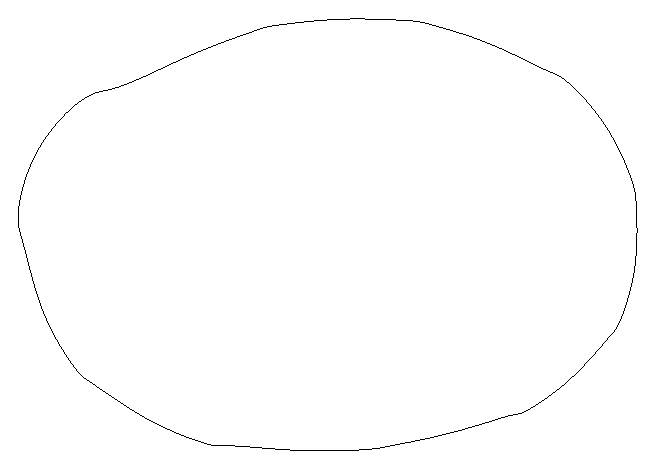
\includegraphics[width=9cm]{Figs/Domain}}
                        \put(2.0,1.7){$\Omega$}
                        \put(3.9,3.0){$\partial\Omega$}
                \end{picture} 
                &
                \setlength{\unitlength}{1cm}
                \begin{picture}(4.5,3.7)
                        \put(0,0){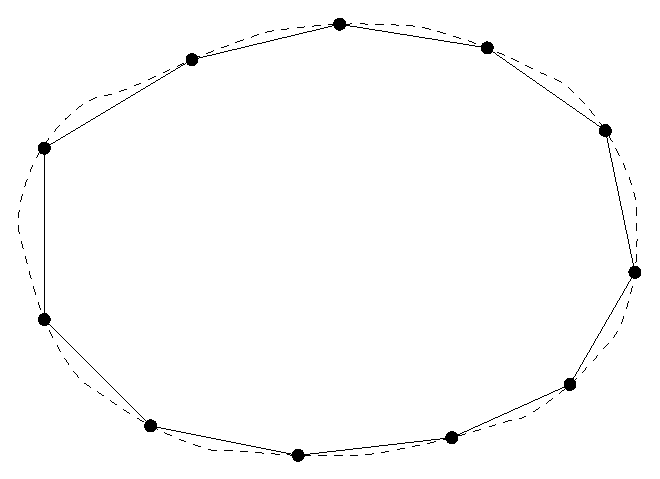
\includegraphics[width=9cm]{Figs/DomainPolygon}}
                        \put(2.0,1.7){$\Omega_{p}$}
                        \put(3.9,3.0){$\partial\Omega_{p}$}
                \end{picture} 
                &
                \setlength{\unitlength}{1cm}
                \begin{picture}(4.5,3.7)
                        \put(0,0){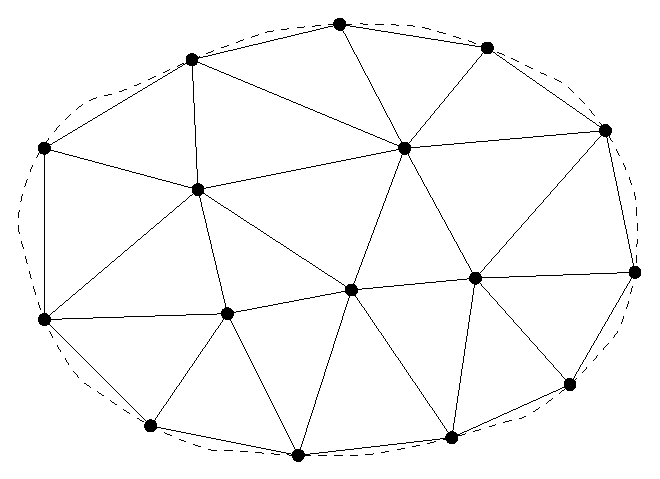
\includegraphics[width=9cm]{Figs/DomainMesh}}
                        \put(2.0,1.7){$\Omega_{h}$}
                        \put(3.9,3.0){$\partial\Omega_{h}$}
                \end{picture}
        \\
        (a) & (b) & (c)
        \end{tabular}
        }
        \caption{(a) Domain of solution, $\Omega$, (b) approximation of $\Omega$ by a polygon, $\Omega_{p}$,  and (c) the mesh of the domain, $\Omega_{h}$.}
\end{figure}

We will examine triangulation further. If we use triangulation then the `elements' are now triangles, $T$.
Usually the triangulation is conforming $\equiv$ the triangles must meet only on a single common edge or vertex.

A virtue of triangulation is that you can refine uniformly or locally as required.

The process of generating `good meshes' involves making the triangles as close to equilateral as possible and is a field in itself called \emph{grid or mesh generation} including ideas of Delaunay and constrained Delaunay triangulations.
REF: Strang and Persson 2001.

\begin{example}
Have a look at the distmesh functions \mcode{meshdemo2d} and \mcode{meshdemond}.
\end{example}

\begin{example}
Have a look online at the tools  \mcode{triangle} (search for ``triangle mesh") and \mcode{tetgen}.
\end{example}


\newpage

\subsubsection{Step 5: finite element space}

Now we need to choose a piecewise polynomial space which is a finite dimensional subspace of our test space.

\vspace{0.5cm}
{\bf Simplest case: Lagrange linear elements, $P_1 \subset C_0$}

Define shape functions on a reference triangle, the canonical triangle.



Any linear function in 2D has the form 
\begin{equation*}
p_1(x,y)=c_1+c_2x+c_3y.
\end{equation*}
Therefore we need 3 basis functions per element. So we need 3 DOF per element, and for a nodal basis we need 3 nodes per element.

If we put the nodes on the vertices (simplest case) then we obtain Lagrange linear triangles (which is what the PDE toolbox in MATLAB uses).

We need 3 shape functions on on the reference triangle which satisfy \mbox{$N_j(v_i)=\delta_{ij}$}.
\begin{align*}
N_1(\xi,\eta)=&1-\xi-\eta,\\
N_2(\xi,\eta)=&\xi,\\
N_3(\xi,\eta)=&\eta.
\end{align*}



We map these shape functions from the reference triangle to a triangle, \mbox{$T=\{(x_1,y_1),(x_2,y_2),(x_3,y_3)\}$}, by an affine transformation:


\begin{equation*}
\begin{bmatrix}
x\\
y
\end{bmatrix}
=
\begin{bmatrix}
x_2-x_1 & x_3-x_1\\
y_2-y_1 & y_3-y_1
\end{bmatrix}
\begin{bmatrix}
\xi\\
\eta
\end{bmatrix}
+
\begin{bmatrix}
x_1\\
y_1
\end{bmatrix},\\
\end{equation*}


\begin{equation*}
\implies \vec{x}=F_T(\vec{s}) ={J}_T\vec{s} +  \vec{b}_T.
\end{equation*}

We can use this to calculate the linear system, e.g. for the element load vectors,

\begin{equation*}
f_{T}=
\begin{bmatrix}
\int_{T} f \phi_i \, dA\\
\int_{T} f \phi_{j} \, dA\\
\int_{T} f \phi_{k} \, dA
\end{bmatrix},
\end{equation*}
we can calculate the entries as
\begin{align*}
\int_{T} f \phi_i \, dA = &\int_{T}f(\vec{x})\phi_j(\vec{x})\, dxdy\\
=&\int_{T_R} f(\vec{x}(\vec{s}))N_j(\vec{s})|\operatorname{det}(J_T)|\, d\xi d \eta.
\end{align*}
Similarly, for the stiffness matrix, 
\begin{equation*}
K_{T}=
\begin{bmatrix}
\int_{T} D\nabla\phi_i\cdot\nabla\phi_i \, dA&
\int_{T} D\nabla\phi_i\cdot\nabla\phi_j \, dA&
\int_{T} D\nabla\phi_i\cdot\nabla\phi_k \, dA&\\
\int_{T} D\nabla\phi_j\cdot\nabla\phi_i \, dA&
\int_{T} D\nabla\phi_j\cdot\nabla\phi_j \, dA&
\int_{T} D\nabla\phi_j\cdot\nabla\phi_k \, dA&\\
\int_{T} D\nabla\phi_k\cdot\nabla\phi_i \, dA&
\int_{T} D\nabla\phi_k\cdot\nabla\phi_j \, dA&
\int_{T} D\nabla\phi_k\cdot\nabla\phi_k \, dA&\\
\end{bmatrix},
\end{equation*}
we can calculate the entries as
\begin{align*}
\int_{T}  D\nabla\phi_i\cdot\nabla\phi_j \, dA 
= &\int_{T} D(\vec{x})\nabla\phi_i(\vec{x})\cdot\nabla\phi_j(\vec{x})\, dxdy\\
= &\int_{T_R} D(\vec{x}(\vec{s}))\left(J_T^{-T}\nabla_{\vec{s}}N_i(\vec{s})\right)\cdot\left(J_T^{-T}\nabla_{\vec{s}} N_j(\vec{s})\right)|\operatorname{det}(J_T)|\, d\xi d\eta.
\end{align*}



\begin{example}[Quadrature rules]
Some quadrature rules on reference triangles $T_R$:
\begin{itemize}
	\item $\int_{T_R}g(\xi,\eta)d\xi d\eta = \frac{1}{2}g(1/3,1/3)$,
	
	\item $\int_{T_R}g(\xi,\eta)d\xi d\eta =
	 \frac{1}{6}\left[g(1/2,0) + g(1/2,1/2) + g(0, 1/2)\right]$,

\end{itemize}

\end{example}



So we have the process:
\begin{itemize}
\item Choose a piecewise polynomial space;
\item Compose each element of $K,M,\vec{f}$;
\item Assemble into global matrices;
\item Impose boundary conditions;
\item Solve linear system; then
\item Plot the solution.
\end{itemize}

\newpage
\subsubsection{Other basis functions}

While you can get a long way with linear basis functions in some cases you may want to use (or need to in some cases, i.e. locking in incompressible solids) higher order functions, or even different shaped elements.

\vspace{0.5cm}
{\bf Triangles: Lagrange quadratic elements, $P_2 \subset C_0$}

Any function in $P_2 \subset C_0$ has the form:
\begin{equation*}
p_2(x,y) = c_1+c_2x+c_3y+c_4x^2+c_5xy+c_6y^2.
\end{equation*}
We have six degrees of freedom per element and therefore we need six nodes per element and the basis functions are extensions of in the 1D case.



\vspace{0.5cm}
{\bf Triangles: Lagrange cubic elements, $P_3 \subset C_0$}

If we want cubic polynomials i.e. $P_3$, then we have 10 degrees of freedom, and need 10 nodes per element


\vspace{0.5cm}
{\bf Rectangles:  $Q_1$: bilinear element}
If we have rectangular elements instead of triangles then our simplest function is
\begin{equation*}
q_1(x,y)=(c_1+c_2x)(c_3+c_4y).
\end{equation*}
Which is linear in both $x$ and $y$ but not linear (it has an $xy$ term which is not in $P_1$).

This has four degrees of freedom, so we need four nodes per  element. On the canonical square (reference element) they are 
\begin{align*}
N_1=&(1-\xi)(1-\eta),\\
N_2=&(1-\xi)\eta,\\
N_3=&\xi(1-\eta),\\
N_4=&\xi\eta.
\end{align*}

\begin{example} 
Run the code \mcode{Shape_rect.m} to see examples of the basis functions.
\end{example}

\newpage
{\bf Rectangles:  $Q_2$: biquadratic element}

Functions in $Q_2$ take the form
\begin{align*}
q_2(x,y)&=(c_1+c_2x+c_3x^2)(c_4+c_5y+c_6y^2)\\ 
      &=c_1c_4+c_2 c_4 x + c_1 c_5y+c_3 c_4 x^2+c_1c_6y^2 + c_2 c_5 xy + c_2 c_6 xy^2 + c_3 c_5 x^2y + c_3 c_6 x^2 y^2,
\end{align*}
which has 9 degrees of freedom, which gives 4 corner shape functions, 4 edge shape functions and 1 bubble function.


\newpage
\subsubsection{Practice time}

\begin{example} 
Solving problems with \mcode{pdetool}
\begin{itemize}
\item using the GUI
\item from the command line $\to$ writing scripts \mcode{Pde2p1.m}
\end{itemize}
\end{example}

\begin{example} 
Now you can understand the code in the built in MATLAB demos (look at them and use \mcode{publish} to see them fully.

\begin{itemize}
\item \mcode{pdedemo1}: solves a Poisson equation on a disc.
\item \mcode{pdedemo2}: solves a Helmholtz equation (spatial part of 
the solution of a wave equation).
\item \mcode{pdedemo3}: solves a nonlinear elliptic equation (soap bubble equation) using 
\mcode{pdenonlin}, which uses damped Newton iterations.
\item \mcode{pdedemo8}: solves a Poisson equation on a square and times \mcode{assempde} against the fast Poisson solver \mcode{poisolv}
\end{itemize}

\end{example}

\begin{example} 
Try the codes in \mcode{fem50}: to run these double click the folder to put it at the top of your path and run
\mcode{clear} and \mcode{close all} before each command. These are all based on the paper `Remarks around 50 lines of Matlab: Short Finite Element Implementation'. 
\begin{itemize}
\item \mcode{fem2d}: solves a 2d Poisson equation on a polygonal domain. 
Uses $P_1Q_1$ elements.
\item \mcode{fem2d_heat}: solves a 2d heat equation using implicit Euler time-stepping (see \S 3.2). At each time step you need to solve a Poisson equation. 
\item \mcode{fem2d_nonlin}: solves a nonlinear elliptic equation (Ginzburg-Landau) by using a Newton Raphson method.
\item \mcode{fem3d}: solves a Poisson equation in a 3D piston. Uses tetrahedral elements. 
\end{itemize}

\end{example}
\begin{example} 
These ideas were later extended in `P2Q2Iso2D = 2D Isoparametric FEM in MATLAB' to use $P_2Q_2$ isoparametric elements i.e. can approximate 
curved boundaries better. The codes are in \mcode{P2Q2}. The driver \mcode{P2Q2Iso2D} is set up to solve test problem 7. I could get problems 2,3,4 and 7 to run. 
\end{example}

\begin{example} 
Starting in the 1980s, the use of local error estimators in FEM codes allowed the development of adaptive refinement i.e. only locally refining the mesh where 
the local error is largest. This greatly improves the efficiency of FEM codes. Try the codes in \mcode{AFEM}. 

Add the folder (and subfolders) \mcode{AFEM@matlab} to the path and run \mcode{demo}. Alternatively add the folder and subfolders to the path and look at the following codes.
A Poisson problem in an L-shaped domain is solved in 3 codes: 
\begin{itemize}
\item \mcode{simple} which refines the mesh uniformly
\item \mcode{Lshape} which adaptively refines the mesh
\item \mcode{Lbig} which generates the finest mesh of all - 117,000 triangles!!
\end{itemize}

\end{example}

\begin{example} 
Many FEM solvers exist, commercial or open source. 

An example I have had installed is called FreeFem++, from France. 

Open an example code from Examples -> Chapter 3 -> membrane.edp

You can see how the problem is specified though a scripting language where you have to specify the weak form of the PDE, the FE space etc. 

Other examples of  FEM tools are \mcode{DealII}, \mcode{LibMesh} (both c++) and \mcode{FEniCS} (python). To find them just search for the names online.
\end{example}


%\begin{example} 
%Another example of a tool which uses FEMs to solve PDEs (often coupled to other systems) is Chaste (www.cs.ox.ac.uk/Chaste) there are some movies in the folder \mcode{ChasteMovies} which should give you a feel of the variety of things that can be done with FEMs.
%\end{example}


\newpage
\subsection{Sparse solvers}

For finite difference and finite element methods (but not spectral solvers) we get large sparse linear systems.

These can't be solved efficiently using standard methods for dense systems e.g.\ LU factorisation or Cholesky factorisation.
\begin{example}
For a finite difference grid, there are 
\begin{itemize}
\item $m\times m$ unknowns, so $N=m^2$ in 2D
\item $m \times m \times m$ unkowns, so $N=m^3$ in 3D
\end{itemize}
A dense Cholesky solver uses $\sim \frac{1}{6}N^3$ operations, so we need
\begin{itemize}
\item $O(m^6)$ operations in 2D
\item $O(m^9)$ operations in 3D
\end{itemize}
But if we count the number of unzero elements in $A$ we have
\begin{itemize}
\item $5m^2$ elements in 2D
\item $7m^3$ elements in 3D
\end{itemize}
which suggests there is a lot of room to improve (our matrices are sparse!).
\end{example}

We have two choices:
\begin{itemize}
\item Sparse direct solvers, which are competitive in 2D
\item Iterative solvers which are ultimately more efficient as we move up in dimensions
\end{itemize}

\newpage

\subsubsection{Direct Sparse methods}
With direct sparse solvers we get exact answers (up to round-off) in principle, but only access the non-zero entries.
MATLAB uses these when using \texttt{\bslash} for sparse systems. 

\begin{itemize}
\item if $A$ is sparse and banded, \texttt{\bslash}  invokes a sparse banded solver, 
\item if $A$ is sparse symmetric, \texttt{\bslash}  invokes sparse Cholesky factorisation.
\end{itemize}

The problem with using a traditional Cholesky directly is that row operations `destroy zeros', i.e. the matrix loses sparsity during factorisation (this is called \emph{fill in}).
The aim is to try and use re-ordering of the equations to minimise fill in. 
\begin{example}{\ }
Run the demo \mcode{sparsity} to see the effect of different orderings on the amount of fill-in using sparse Cholesky. On current desktop machines, the speedup from 
reordering is not apparent on the example matrix. See \mcode{MySparsity} for the same example with a different larger matrix, what is the best reordering now? 
\end{example}

After much research into different orderings, MATLAB uses \mcode{ammd} by default, but you can choose a different ordering if you want. For details, see Davis, SIAM, 2007. 

Sparse Cholesky uses a re-ordering automatically  and only handles non-zero elements, resulting in
\begin{itemize}
\item  $O(m^3)$ operations in 2D (c.f. $O(m^6)$) and
\item $O(m^6)$ operations in 3D (c.f. $O(m^9)$)
\end{itemize}

PDE toolbox in MATLAB in fact uses \texttt{\bslash} to solve finite element equations. FreeFem++ uses iterative methods. 

From personal experience we've found \texttt{\bslash} fastest in MATLAB for 2D problems, because \texttt{\bslash} is compiled while iterative solvers are interpreted.
 In 3D, iterative solvers start to do better. In compiled languages (C++), iterative approaches are usually better off the bat. 

\newpage

\subsubsection{Iterative solvers}
There are three main classes of iterative solvers:
\begin{itemize}
\item Classical stationary (1950s)
\item Krylov space methods: (1970s-1990s)
\item Multigrid methods (1980s-)
\end{itemize}

There are two main reasons to look at iterative solvers for sparse systems:
\begin{itemize}
\item More Efficiency

Each iteration typically involves a matrix-vector product $Av$, for finite difference with a 5 point stencil, $A$ has 5 non-zero entries per row and $A$ is $m^2 \times m^2$ so to form $Av$ takes $5m^2$ operations, for finite element methods $A$ has 9 non-zero entries per row so to form $Av$ takes $9m^2$ operations.

So in 2D as long as our solver converges in $O(m)$ iterations, we can achieve $O(m^3)$ complexity running time which matches (asymptotically) sparse Cholesky.

In 3D we only have $Lm^3$ operations per iteration so we require  $O(m^3)$ iterations for convergence to do equal to or better than sparse Cholesky. 

\item The matrix $A$ is not exact.

We already have a discretisation error $O(h^2)$ (local truncation error), so the residual is $O(h^2)$.
Why use a solver whose relative residuals are $O(u)$ (unit round-off) when the backward error in $A$ is $O(h^2)$?
Instead, aim to solve $Au=F$ approximately till residual is $O(h^2)$ -- this is not possible with direct methods.
\end{itemize}

We will look only at Krylov subspace methods. (Others covered in Student talks).

\newpage
\subsubsection{Krylov subspace methods}

For $A$ symmetric positive definite, e.g.\ FD/FEM discretisations of elliptic PDEs,
the best iterative method is called \emph{preconditioned conjugate gradient (PCG)}. 
This is one member of a large class of methods developed over 1971-1995 that have become 
current standard practice. 



Refs: Trefethen \& Bau, Elman et. al Chapter 2, Johnson Chapter 7, Braess Chapter 4, 
Gockenbach Chapter 11, Kelley, Iserles, Schewchuk. 



We will start with gradient methods, move to conjugate gradient methods and then move onto preconditioned conjugate gradient methods.

Conjugate gradient methods started out as an optimisation algorithm (1952 Ref: Hestenes \& Stiefel) and were later re-used as an iterative solver (1971).


{\bf \nth{1} Observation}: 
$\mbox{ find the solution of $A\vec{x}=\vec{b}$} \equiv \mbox{ find the minimum of $\phi(x)$}$, where $\phi(x)=\frac{1}{2}\vec{x}^TA\vec{x}-\vec{b}^T\vec{x}$.

If $A$ is symmetric positive definite, $\phi(x)$ has a global minimum at $\vec{x}^*=A^{-1}\vec{b}$ 

Recall: $A$ is positive definite if $\vec{x}^TA\vec{x} \ge 0$ and the equality holds if and only if $\vec{x}=\vec{0}$.

Aim: find this minimum as fast as possible (in as few iterations as possible).

\newpage
\subsubsection{Gradient method (steepest descent)}

Tip from Newton's method: use $\nabla \phi$ to tell us a descent direction $\vec{p}$.

Since the directional derivative of $\phi$ in the direction $\vec{d}$ (a unit vector)  is $\nabla \phi \cdot \vec{d}$,
 this is minimised if $\vec{d}$ is in the direction $-\nabla\phi$ which implies that $-\nabla \phi$ is the direction of steepest descent.

At current guess $\vec{x}_k$: 
\begin{itemize}
\item Compute descent direction, $\vec{d}_k=-\nabla \phi\big|_{\vec{x}_k}$.
\item Step along $\vec{d}_k$ in a line search a distance $\alpha_k$, chosen to give the minimum possible value of $\phi$.
\end{itemize}
\begin{align*}
&\min_{\alpha \ge 0} \phi(\vec{x}_k+\alpha\vec{d}_k).
\end{align*}
So
\begin{align*}
 & \frac{d}{d\alpha} \phi(\vec{x}_k + \alpha\vec{d}_k)=0\\
\implies &\nabla\phi\big|_{\vec{x}_k+\alpha\vec{d}_k} \cdot \vec{d}_k=0\\
\implies& \nabla\phi\big|_{\vec{x}_{k+1}} \cdot \vec{d}_k =0
\implies \mbox{ so $\vec{d}_{k+1} \perp \vec{d}_k$}.
\end{align*}
This means we will follow a zig-zag path.

Since $\nabla \phi = Ax -b$, $\vec{d}_k = - \nabla \phi = b-A\vec{x}_k=\vec{r}_k$, the orthogonality of 
$\vec{d}_k$ and $\vec{d}_{k+1}$ 
\[\vec{d}_k \cdot \underbrace{[b-A(\vec{x}_k +\alpha_k\vec{d}_k)]}_{\vec{d}_{k+1}}=0,\]
give an equation for $\alpha_k$:
\begin{equation*}
\alpha_k=\frac{\vec{d}_k \cdot (\vec{b}-A\vec{x}_k)}{\vec{d}_k \cdot A\vec{d}_k} = \frac{\vec{r}_k^T \vec{r}_k}{\vec{r}_k^T A \vec{r}_k},
\end{equation*}
in terms of the \emph{residual} $\vec{r}_k = \vec{b}-A\vec{x}_k$.
Iterating these steps gives the {\bf  steepest descent algorithm}.



\newpage
{\bf  Steepest descent algorithm:}
\begin{verbatim}
Choose x_0
repeat
     r_k = b - A x_k
     stopping criterion here
     alpha_k = r_k^T r_k/( r_k^T A r_k)
     x_k+1 = x_k + alpha_k r_k
end
\end{verbatim}
which can be reorganised (Ref: Leveque p. 80) to a version which only uses 1 matrix-vector product per iteration:
\begin{verbatim}
Choose x_0
r_0 = b-A x_0
repeat k = 1,2, ...
     w_{k-1} = A r_{k-1}
     alpha_{k-1} = r_{k-1}^T r_{k-1}/(r_{k-1}^T w_{k-1})
     x_k = x_{k-1} + alpha_{k-1} r_{k-1}
     r_k = r_{k-1} - alpha_{k-1} w_{k-1}        
     stopping criterion here
end
\end{verbatim}

the last step using
\begin{align*}
\vec{r}_k=&\vec{b}-A\vec{x}_k\\
=&\vec{b}-A(\vec{x}_{k-1}+\alpha_{k-1}\vec{r}_{k-1})\\
=&\vec{r}_{k-1}-\alpha_{k-1}\vec{w}_{k-1}
\end{align*}

This always finds the minimum, but it may be very slow.
\begin{example} If $A=I$ it in fact finds the minimum in one step, but if 
\begin{equation*}
A=
\begin{pmatrix}
\lambda_1 & 0 \\
0& \lambda_2
\end{pmatrix},
\end{equation*}
and $\lambda_1 \gg \lambda_2$, then we get a `zig-zagging' pattern and it takes a long time to converge.

\end{example}
%\newpage
% $\min,\max$

\begin{thm}
If $A$ is symmetric positive definite with condition number 
\begin{align*}
\kappa_2(A) = \frac{\lambda_{\max} (A)}{\lambda_{\min} (A)},
\end{align*}
then the steepest descent algorithm converges according to
\begin{equation*}
\|\vec{e}_k\|_A \le \left(\frac{\kappa-1}{\kappa+1}\right)^k\|\vec{e}_0\|_A,
\end{equation*}
where we have used a new norm for the error 
\begin{equation*}
\|\vec{x}\|_A=(\vec{x}^TA\vec{x})^{\frac{1}{2}},
\end{equation*}
which has the properties of a norm only if $A$ is spd. 
\end{thm}
\begin{example}
for $A=I$, $\|\vec{x}\|_A=\|\vec{x}\|_2$.
\end{example}


\begin{example}
\begin{equation*}
\mbox{If } A=
\begin{pmatrix}
\lambda_1 & 0 \\
0 & \lambda_2
\end{pmatrix}
\mbox{ then }
\|\vec{x}\|_A=\sqrt{x_1^2\lambda_1+x_2^2\lambda_2}
\end{equation*}
\end{example}

The theorem above implies that if $\kappa_2(A)\gg 1$, the convergence is slow since $\frac{\kappa-1}{\kappa+1} \rightarrow 1$.
 See Schewchuk, Fig.20.


\begin{example}
\ if $\lambda_1 \gg \lambda_2$, $\kappa_2 = \frac{\lambda_1}{\lambda_2} \gg 1$.
\end{example}

{\bf The method of steepest descent slows down for ill-condition matrices.}
 
 \newpage
This is relevant to us: 
\begin{itemize}
\item For a finite difference  5-point stencil, the matrix $A$ that we obtain has $\kappa_2(A) \sim h^{-2}$
\item For FEM + nodal basis ($P_m, Q_m, m \ge 1$) gives matrices with $\kappa_2(A) \le C h^{-2}$
\item For a uniform mesh on a square we have $\kappa_2(A) = \frac{2}{\pi^2h^2}+O(1)$
\end{itemize}
So as we refine our mesh to get smaller error, $\kappa_2(A)$ grows and steepest descent slows down.
There are other FEM meshes (hierarchical meshes) that have smaller condition numbers. 

We can estimate the number of iterations required to reduce the error below a specified tolerance $\epsilon$.
\begin{equation*}
\mbox{Want } \left( \frac{\kappa -1}{\kappa+1} \right)^n < \epsilon.
\end{equation*}
Where
\begin{equation*}
\frac{\kappa-1}{\kappa+1}=1-\frac{2}{\kappa+1} \sim 1- \frac{2}{\kappa}, \qquad \mbox{for large $\kappa$}.
\end{equation*}

So we have
\begin{align*}
&n\log\left(1-\frac{2}{\kappa}\right) < \log(\epsilon),\\
\implies &\frac{-2n}{\kappa} < \log(\epsilon), &&\mbox{by  Taylor approximation (as $\frac{2}{\kappa}$ is small)}\\
\implies &n > \log\left(\frac{1}{\epsilon}\right) \frac{\kappa}{2},\\
& \mbox{i.e. } n \propto \kappa_2(A).
\end{align*}

In 2D, $\kappa_2(A) \sim h^{-2} \sim m^2$ for an $m  \times m$ grid,
so \begin{align*}
\mbox{Total work} \sim& \mbox{ \#iterations} \times \mbox{ ops/iteration}\\
=&m^2 \times 5m^2\\
=&O(m^4).
\end{align*}
which is worse asymptotically than sparse Cholesky factorisation. 

\begin{aside}
In 3D, $\kappa_2(A) \sim h^{-2}$ as well, so we use $O(m^5)$ operations to solve our system -- this is already better than sparse Cholesky. But, for the \nth{4} order biharmonic equation arising in elasticity, $\nabla^2\nabla^2u=f$, $\kappa_2(A) \sim h^{-4}$ i.e. slowdown is worse. 
\end{aside}

BUT: we can do better than this with the Conjugate Gradient method.

\newpage
\subsubsection{Conjugate Gradient method}
Idea: Choose different directions $\vec{p}_k$, constructed from steepest descent directions $\vec{r}_k$, which have very nice properties.

In particular, once we have searched along a particular direction, we never want to search in that direction again.
We ensure this by:
\begin{align*}
&\mbox{$\vec{x}_1$ minimises $\phi$ when searching over $\{\vec{p}_1\}$ [as before]}\\
&\mbox{$\vec{x}_2$ minimises $\phi$ when searching over span$\{\vec{p}_1,\vec{p}_2\}$} \mbox{ [not true of steepest descent]} \\
&\mbox{$\vec{x}_3$ minimises $\phi$ when searching over span$\{\vec{p}_1,\vec{p}_2,\vec{p}_3\}$}\\
&\phantom{asdfasdfasfdasdasdsd}\vdots
\end{align*}
By making $x_k$ minimise $\phi$ over nested subspaces, 
we never `backtrack' or search along previous directions, so 
\[\phi(\vec{x}_{k+1}) \le \phi(\vec{x}_k),\]
i.e. $\phi$ decreases monotonically.

The hard part: making this cheap.

We want to construct $\{\vec{p}_j\}$ so that
\begin{align*}
\alpha_k =\min_\alpha \phi(\vec{x}_{k-1}+\alpha \vec{p}_k)
\end{align*}
 also minimises $\phi$ over $x \in \operatorname{span}\{\vec{p}_1,\ldots,\vec{p}_k\}$.

%Choose search directions $\{p_0,p_1,p_2,\ldots\}$ constructed from descent directions $\{r_0,r_1,r_2,\ldots\}$ with the property that:
%
%\begin{align*}
%&x_1: \mbox{minimises $\phi$ over $\{p_0\}$}\\
%&x_2: \mbox{minimises $\phi$ over $\{p_0,p_1\}$}\\
%&x_3: \mbox{minimises $\phi$ over $\{p_0,p_1,p_2\}$}
%\end{align*}

Let's try generating $ \vec{p}_1$:
\begin{enumerate}
\item  Guess $\vec{x}_0, \vec{p}_0$ [often $\vec{x}_0=\vec{0}$, $\vec{p}_0 = \vec{r}_0 =\vec{b}$]
\item Find $\alpha_0$ by a 1D minimisation of $\phi(\vec{x}_0+\alpha \vec{p}_0)$
\begin{align*}\vec{p}_1
\phi(\vec{x}_0 + \alpha \vec{p}_0) =& \frac{1}{2} (\vec{x}_0+\alpha \vec{p}_0)^T A (\vec{x}_0 + \alpha \vec{p}_0) - (\vec{x}_0 + \alpha \vec{p}_0)^T \vec{b}\\
=& \frac{1}{2}\vec{x}_0^TA \vec{x}_0 - \vec{x}_0^T \vec{b} + \frac{1}{2} \alpha^2 \vec{p}_0^T A \vec{p}_0 + \alpha \vec{p}_0^T A \vec{x}_0 - \alpha \vec{p}_0^T \vec{b},
\end{align*}
\begin{equation*}
\frac{d}{d \alpha}(\phi(\vec{x}_0 + \alpha \vec{p}_0) =\vec{0} \implies \alpha \vec{p}_0^T A \vec{p}_0 = \vec{p}_0^T(\vec{b}-A\vec{x}) = \vec{p}_0^T \vec{p}_0,
\end{equation*}
so that we get
\begin{align*}
\alpha_0 =& \frac{\vec{p}_0^T \vec{p}_0}{\vec{p}_0^T A \vec{p}_0},\\
\vec{x}_1 =& \vec{x}_0 + \alpha_0 \vec{p}_0,\\
\vec{r}_1 =& \vec{r}_0 - \alpha_0 \underbrace{A\vec{p}_0}_{\vec{w}_0},
\end{align*}
as for the first step of steepest descent% but with $\vec{p}_0$ so far unspecified. 
\item Find $\vec{x}_2$ by 2D minimisation of
\begin{align*}
\phi(\vec{x}_0 + \alpha \vec{p}_0 + \beta \vec{p}_1) =& \phi(\vec{x}_1 + \beta \vec{p}_1)\\
=&\frac{1}{2}(\vec{x}_1 + \beta \vec{p}_1)^T A (\vec{x}_1 + \beta \vec{p}_1) - (\vec{x}_1 + \beta \vec{p}_1)^T \vec{b}\\
=& \underbrace{\frac{1}{2}\vec{x}_1^TA\vec{x}_1 - \vec{x}_1^T\vec{b}}_{\phi(\vec{x}_1)} + \frac{1}{2} \beta^2 \vec{p}_1^T A \vec{p}_1 + \underbrace{\beta \vec{p}_1^T A \vec{x}_1 - \beta \vec{p}_1^T \vec{b}}_{-\beta \vec{p}_1^T\vec{r}_1}\\
=&\phi(\vec{x}_1) + \frac{1}{2} \beta^2 \vec{p}_1^T A \vec{p}_1 - \beta \vec{p}_1^T(\vec{r}_0 - \alpha A \vec{p}_0),
\end{align*}
where we note that $\beta\alpha \vec{p}_1^TA\vec{p}_0$ is the only term that includes $\beta$ and $\alpha$. 

We can de-couple the 2D minimisation of $\phi$ into two 1D minimizations if we set  this term to zero by choosing
\[\vec{p}_1^TA\vec{p}_0=0.\] 
\end{enumerate}
With this choice of search directions, we turn k-dimensional minimisation over nested subspaces into successive 1D minimisation problems, with no backtracking.

\subsubsection*{Conjugate directions}

Two vectors that satisfy $\vec{u}^{\rm T}A \vec{v}=0$ are called \emph{$A$-conjugate}.

If $A$ is symmetric we can define an inner product $( \vec{u},\vec{v} )_A \equiv \vec{u}^T A\vec{v}$.
If $A$ is also positive definite, this induces a norm $\|\vec{u}\|^2_A \equiv <\vec{u}, \vec{u}>_A= \vec{u}^T A\vec{u}$. So A-conjugate vectors are orthogonal wrt the 
A-inner product. 

We aim to produce a set of mutually A-conjugate vectors. 
To achieve this we do conjugate Gram-Schmidt to form $\{\vec{p}_0,\vec{p}_1,\ldots\}$, from $\{\vec{r}_0,\vec{r}_1,\ldots\}$.

\begin{enumerate}
\item Guess $\vec{p}_0=\vec{r}_0$.
\item Let \begin{align*}
\alpha_0 = & \frac{\vec{r}_0^T\vec{r}_0}{\vec{p}_0^TA\vec{p}_0},\\
\vec{x}_1 = & \vec{x}_0+\alpha_0\vec{p}_0,\\
\vec{r}_1 = & \vec{r}_0-\alpha_0A\vec{p}_0,
\end{align*}
as before. 
\item Now 
\begin{align*}
\vec{p}_1 = & \vec{r}_1 - \mbox{component of $\vec{r}_1$ not $A$-conjugate to $\vec{p}_0$}\\
= & \vec{r}_1 + \beta_0 \vec{p}_0 \qquad \mbox{(since span $\{\vec{r}_0,\vec{r}_1\}=$span $\{\vec{p}_0,\vec{p}_1\}$)}
\end{align*}
Determine $\beta_0$ by enforcing $A$-conjugacy
\begin{align*}
&\vec{p}_1^T A \vec{p}_0 = 0 \implies (\vec{r}_1 + \beta_0\vec{p}_0)^T A \vec{p}_0=0,\\
\implies& \beta_0=\frac{-\vec{r}_1^TA\vec{p}_0}{\vec{p}_0^TA\vec{p}_0}.
\end{align*}
Then since
\begin{equation*}
\vec{r}_1=\vec{r}_0-\alpha_0 A \vec{p}_0, \qquad -A\vec{p}_0=\frac{\vec{r}_1-\vec{r}_0}{\alpha_0},
\end{equation*}
\begin{align*}
\beta_0=&\frac{\vec{r}_1^T (\vec{r}_1-\vec{r}_0)/\alpha_0}{\vec{p}_0^T A\vec{p}_0}\\
=& \frac{\vec{r}_1^T \vec{r}_1}{\alpha_0 \vec{p}_0^T A \vec{p}_0}\\
=&\frac{\vec{r}_1^T \vec{r}_1}{\vec{r}_0^T \vec{r}_0}, \qquad(=\mbox{reduction in the square residual.})
\end{align*}

\item So given $\vec{p}_1$, $\vec{x}_1$, $\vec{r}_1$, we calculate $\vec{p}_2$:
\begin{align*}
\alpha_1 = \frac{\vec{r}_1^T\vec{r}_1}{\vec{p}_1^T A \vec{p}_1}, \qquad x_2=\vec{x}_1+\alpha_1 \vec{p}_1, \qquad \vec{r}_2= \vec{r}_1-\alpha_1 A \vec{p}_1,\\\
\beta_1=\frac{\vec{r}_2^T\vec{r}_2}{\vec{r}_1^T\vec{r}_1}, \qquad \vec{p}_2=\vec{r}_2+\beta_1 \vec{p}_1.
\end{align*}

This all leaves $\vec{r}_2 \perp \vec{r}_0, \vec{r}_1$; $\vec{p}_2$  conjugate to $\vec{p}_0, \vec{p}_1$; and  $\vec{r}_2 \perp \vec{p}_0, \vec{p}_1$ (but not $\vec{p}_2$.

\end{enumerate}
After $k$ iterations, 
\begin{align*}
\vec{x}_k= \mbox{solution that minimizes $\phi$ over $x \in \vec{x}_0+\mbox{span}\{\vec{p}_0,\vec{p}_1,\ldots,\vec{p}_{k-1}\}$}
\end{align*}

Minimising $\phi$ is same as minimising the error in the $A$-norm:\\$\|\vec{e}\|_A=\|\vec{x} -\vec{x}^*\|_A$.

\begin{proof}
\begin{align*}
\|\vec{e}\|^2_A =& \|\vec{x}-\vec{x}^*\|_A^2 = (\vec{x}-\vec{x}^*)^TA(\vec{x}-\vec{x}^*)\\
=& \vec{x}^TA\vec{x} - 2\vec{x}^TA\vec{x}^*+\vec{x}^{*T}A\vec{x}^*\\
=& \underbrace{\vec{x}^TA\vec{x} - 2\vec{x}^T\vec{b}}_{2\phi(\vec{x})} + \underbrace{\vec{x}^{*T}A\vec{x}^*}_{\mbox{constant}}
\end{align*}
\end{proof}

$\vec{x}_k$ minimises $\|\vec{e}\|_A$ over $\vec{x}_0 + \mbox{span}\{\vec{p}_0, \ldots, \vec{p}_{k-1}\}$. But

\begin{equation*}
\vec{r}_0=\vec{p}_0,\vec{r}_1=\vec{r}_0-\alpha_0 A \vec{p}_0,\vec{r}_2=\vec{r}_1 - \alpha_1 A\vec{p}_1. \ldots
\end{equation*}
so
\begin{equation*}
\mbox{span}\{\vec{p}_0,\vec{p}_1,\ldots,\vec{p}_{k-1}\} = \underset{\mbox{Krylov Space}}{\mbox{span} \{\vec{r}_0, A\vec{r}_0, A^2,\ldots,A^{k-1}\vec{r}_0\}}.
\end{equation*}

Since $A\vec{x}=\vec{b}-\vec{r}$ and $A\vec{x}^*=\vec{b}$, $A\vec{e}=-\vec{r}$, so
\begin{align*}
\mbox{span}\{\vec{p}_0,\vec{p}_1,\ldots,\vec{p}_{k-1}\} =& \mbox{span} \{\vec{r}_0, A\vec{r}_0, A^2,\ldots,A^{k-1}\vec{r}_0\}\\ =& \mbox{span}\{A\vec{e}_0,A^2\vec{e}_0,\ldots,A^k\vec{e}_0\}
\end{align*}
so 
\begin{equation*}
\vec{x}_k = \vec{x}_0 + \mbox{Linear combinations}\{A\vec{e}_0,\ldots,A^k\vec{e}_0\}
\end{equation*}

If we subtract $\vec{x}^*$ from both sides then
\begin{equation*}
\vec{e}_k=\vec{e}_0+\mbox{Linear combinations}\{A\vec{e}_0,\ldots,A^k\vec{e}_0\} = P_k(A)\vec{e}_0
\end{equation*}
where $P_k$ is a polynomial of degree k with $p(0)=1$ (\emph{monic polynomial}).

Since conjugate-gradient minimises $\phi(x)$ and $\|\vec{e}\|_A$ over $\mathcal{K}_k$, 
\begin{equation*}
\|\vec{e}_k\|_A = \min_{p \in P_k} \|p(A)\vec{e}_0\|_A.
\end{equation*}

Also we have $\|\vec{e}_{k+1}\|_A \le \|\vec{e}_k\|_A$ since $\mathcal{K}_{k+1} \supset \mathcal{K}_k$ (or since $\phi(x_{k+1}) \le \phi(x_k)$).
After $N$ steps, (where $A$ is $N\times N$, ($N=m^2$ in 2D)), we have $\vec{e}_N=\vec{0}$ (up to round-off), 
since $\mathcal{K}_N = \R^n$ or since $A$ satisfies its characteristic polynomial $p_N(A)=0$.

{\bf Conjugate gradient converges to the exact answer in $N$ iterations (ignoring roundoff).}
Conjugate gradient is guaranteed to converge in $N$ (which is $m^2$ or $m^3$) iterations, but its use depends on fast convergence in $k \ll N$ iterations.

Another way to characterise the convergence of CG: 
\begin{equation*}
\frac{\|\vec{e}_k\|_A}{\|\vec{e}_0\|_A}=\inf_{p \in P_k} \frac{\|p(A)\vec{e}_0\|_A}{\|\vec{e}_0\|_A}.
\end{equation*}

Expand $\vec{e}_0$ in eigenvectors of $A$: $\vec{e}_0=\sum a_j \vec{v}_j$ (orthonormal) then $p(A)\vec{e}_0 = \sum a_j p(\lambda_j)\vec{v}_j$.
\begin{align*}
\implies \|\vec{e}_0\|^2_A = \vec{e}_0^T A \vec{e}_0=& \sum_k a_k \vec{v}_k^T \sum_j a_j \lambda_j \vec{v}_j\\
=& \sum_k a_k \delta_{kj} \sum a_j \lambda_j\\
=&\sum_j a_j^2 \lambda_j
\end{align*}
Similarly
\begin{equation*}
\|p(A)\vec{e}_0\|^2_A = \sum a_j^2 p(\lambda_j)^2\lambda_j
\end{equation*}
So
\begin{equation*}
\frac{\|p(A)\vec{e}_0\|_A}{\|\vec{e}_0\|_A} = \frac{\sum a_j^2 p(\lambda_j)^2 \lambda_j}{\sum a_j^2 \lambda_j} \le \max_{\lambda \in \Lambda(A)}p(\lambda)^2
\end{equation*}
\begin{equation*}
\implies \frac{\|\vec{e}_k\|_A}{\|\vec{e}_0\|_A} \le \inf_{p \in P_k} \max_{\lambda \in \Lambda(A)} p(\lambda)^2
\end{equation*}

{\bf The convergence of CG is determined by how small a polynomial with $p(0)=1$ can be at the eigenvalues of $A$, i.e.\ it is determined by the spectrum of $A$.}

\begin{example}
If $A$ has only $k <N$ different eigenvalues  then conjugate gradient converges in $k$ iterations.
\begin{proof}
The polynomial of degree $k$:
\begin{equation*}
\prod_{i=1}^k \left(1- \frac{x}{\lambda_i}\right),
\end{equation*}
has $p(0)=1$, but $p(\lambda_i)=0 \implies \vec{e}_k=\vec{0}.$
\end{proof}
\end{example}

\newpage
{\bf Conjugate gradient converges fast if the eigenvalues are grouped in a few clusters: }

 
 \begin{example}
If we don't know the spectrum of $A$ but only know $\lambda \in (\lambda_{\min},\lambda_{\max})$, then the best result is:
\begin{equation}\label{CGcgce}
\frac{\|\vec{e}_k\|_A}{\|\vec{e}_0\|} \le 2 \left( \frac{\sqrt{\kappa}-1}{\sqrt{\kappa}+1} \right)^k,
\end{equation}
where $\kappa = \kappa_2(A) = \frac{\lambda_{\max}}{\lambda_{\min}}$.
\end{example}

So if $\kappa$ is near 1, i.e. $\lambda_{\max} - \lambda_{\min} \ll \lambda_{\max} + \lambda_{\min}$, then convergence is rapid.

But this bound can be pessimistic,
so if $\kappa \gg 1$, convergence \emph{could} be slow but the previous result, $\inf \max |p(\lambda)|$, is a tighter bound.
i.e. the  clustering of eigenvalues determines convergence, not just their range.

Using the bound in Equation \ref{CGcgce}, we can estimate a (pessimistic) bound for the number of iterations to achieve a tolerance $\epsilon$:
\[n > \frac{\sqrt{\kappa}}{2} \log\left(\frac{2}{\epsilon}\right).\]
So we need $\sim \sqrt{\kappa}$ iterations for CG to achieve convergence. 

\begin{example}
For a 5-point FD stencil or $P_1$ or $Q_1$ FEM, $\kappa_2 \sim h^{-2} \sim m^2$.
So if we require $\sim\sqrt{\kappa_2}$ iterations then the total work is $O(m^3)$ to find the solution -- the same complexity as \texttt{\bslash} in 2D.

In 3D we have $\sim m$ iterations at $O(m^3)$ operations per iteration, so $O(m^4)$, compared to $O(m^6)$ for \texttt{\bslash}.
\end{example}

CG is the \nth{1} example we have seen  where an iterative process depends on the spectrum of the matrix.
 
\newpage
{\bf Stopping Criterion:}

We want to know when to stop; we can't stop using $\| \vec{e}_k \|_A$ since we can't compute it. 
But $A\vec{e}_k=-\vec{r}_k$, $A\vec{e}_0=-\vec{r}_0$, so $\vec{e}_k=-A^{-1}\vec{r}_k$, $\vec{e}_0=-A^{-1}\vec{r}_0$.
So we have
\begin{align*}
\|\vec{e}_k\|^2_A =& \vec{e}_k^TA\vec{e}_k=\vec{r}_k^TA^{-T}AA^{-1}\vec{r}_k=\vec{r}_k^TA^{-1}\vec{r}_k, \qquad ( \mbox{ since }A \mbox{ symmetric})\\
\|\vec{e}_0\|_0^2 =& \vec{r}_0^T A^{-1}\vec{r}_0,
\end{align*}
where $A^{-T}(=A^{-1})^T$.
\begin{align*}
\vec{r}_k^T A^{-1} \vec{r}_k \le& \lambda_{\max}(A^{-1})\vec{r}_k^T\vec{r}_k,\\
\vec{r}_0^T A^{-1}\vec{r}_0 \ge& \lambda_{\min}(A^{-1})\vec{r}_0^T \vec{r}_0.
\end{align*}

So
\begin{align*}
&\frac{\|\vec{e}_k\|^2_A}{\|\vec{e}_0\|_A^2} \le \underbrace{\frac{\lambda_{\max}(A^{-1})}{\lambda_{\min}(A^{-1})}}_{=\frac{\lambda_{\max}(A)}{\lambda_{\min}(A)}=\kappa_2(A)} \frac{\|\vec{r}_k\|^2}{\|\vec{r}_0\|^2}\\
\implies& \frac{\|\vec{e}_k\|_A}{\|\vec{e}_0\|_A} \le \sqrt{\kappa_2(A)}\frac{\|\vec{r}_k\|}{\|\vec{r}_0\|}
\end{align*}
so we can use $\|\vec{r}_k\|$ or $\frac{\|\vec{r}_k\|}{\|\vec{r}_0\|}$ as a stopping criterion as a proxy for $\|\vec{e}_k\|_A$.

Since the local truncation  error of discretisation (i.e.  the residual $A\vec{x} -\vec{b}$) is $O(h^2)= O(m^{-2})$ anyway (for $P_1$/$Q_1$ etc. ), often we use $\|\vec{r}_k\| \le ch^2$ as a stopping criterion, rather than a fixed stopping tolerance $\epsilon$ 
i.e. the finer the discretisation, the tighter the stopping criterion, so we expect more iterations as $h$ decreases, when compared to a fixed tolerance.
But the effect is quite weak: if we use $\|\vec{r}_k\| \le ch^2$ then $n > \sqrt{\kappa} |\log h|$ instead of $\sqrt{\kappa}$.

To see the effect of the spectrum on the convergence of CG, the following graph shows the convergence for 4 $100 \times 100$ matrices, with different spectra. 
%\vspace{5cm}
\begin{figure}[H]
   \includegraphics[scale = 0.8]{CG_test} % requires the graphicx package
 \caption{Convergence of CG for matrices of different spectra}
\end{figure}

Since CG converges faster if the spectrum is `nice', we look for ways to improve the spectrum, i.e. \textbf{preconditioning}.

\newpage
\subsubsection{Preconditioned conjugate gradient (PCG)}

Instead of solving $A\vec{x}=\vec{b}$, solve $M^{-1}A\vec{x}=M^{-1}\vec{b}$ such that:
\begin{itemize}
\item  it must be cheap to solve $M\vec{z}=\vec{r}$ (which is the only place $M$ enters in the PCG algorithm)
\item $M^{-1}A$ must be sparse and symmetric positive definite (if $A$ is)
\item $M^{-1}A$ has a `nicer' spectrum, e.g.\ $\kappa_2(M^{-1}A) \ll \kappa_2(A)$
\end{itemize}
These are conflicting requirements.

\begin{example}
If $M=I$ then $M\vec{z}=\vec{r}$ is easy to solve, but $\Lambda(M^{-1}A) = \Lambda(A)$ and we haven't done anything.
\end{example}
\begin{example}
If $M=A$ now $\Lambda(M^{-1}A) = \Lambda(I)$ which is perfect but $M\vec{z}=\vec{r}$ is $A\vec{z}=\vec{r}$ which is just our original problem.
\end{example}

We try and look for $M$ that `approximates' $A$ so that the eigenvalues of $M^{-1}A$ are more clustered than $A$.
We often look for a factorised $M=M_1M_2$ where $M_1$, $M_2$ are cheap to invert, e.g.\ Cholesky factors $M = L L^T = R^T R$

{\bf There are \emph{no} magical preconditioners!}

The best comes from a deep knowledge of $A$ and where it came from.
They  often come from approximating $A$ or solving a related simpler problem cheaply to get an approximation.

Some candidates that are symmetric positive definite and sparse:
\begin{itemize}
\item Jacobi (point), $M_J = D = \operatorname{diag}(A)$.

This has modest benefit unless the diagonal elements of $A$ vary greatly.  It has no effect on $A_5$ (since the diagonal elements are all the same).

\item Incomplete factorisations

For these we go through the process of (Cholesky) factorisation but prevent or reduce the amount of fill-in.
So the matrix obtained is sparser than usual sparse Cholesky factorisation (less fill-in) but only gives an approximate factorisation.

Direct Cholesky (\texttt{\bslash})
\begin{equation*}
A=R^TR \mbox{ or } L L^T.
\end{equation*}

Incomplete Cholesky
\begin{equation*}
A= \bar{R}^T \bar{R} + \underbrace{\epsilon}_{\mbox{error}},
\end{equation*}
where $\bar{R}^T\bar{R}=M$ is  a preconditioner, $M=M_1M_2=\bar{R}^T\bar{R}$ ( or $M = \bar{L}\bar{L}^T$).

MATLAB has (as at 2012):
\begin{itemize}
\item Incomplete Cholesky with no fill-in 

\mcode{L = ichol(A)}, which you then use in a call to \mcode{pcg}:

\mcode{[  ,   ,   ,  ] = pcg(A,b,tol,maxits, L, L')}

This only allows non-zeroes of $L$ where $A$ has non-zeroes i.e. no fill-in.
To call CG in MATLAB, use \mcode{pcg} with no preconditioner:

\mcode{[  ,   ,   ,  ] = pcg(A,b,tol,maxits)}

\item Modified incomplete Cholesky

Where the matrix $A$ has come from an elliptic PDE (as in our cases), it is better when you delete an entry that would  have produced fill-in 
to add that entry to the diagonal entry on the same row, so that $A\vec{x} = \bar{L}\bar{L}^T\vec{x}$ when $\vec{x}$ is a constant vector. This is called 
Modified incomplete Cholesky (MIC) factorization. This can be called in MATLAB by accessing the \mcode{options} structure in the call to \mcode{ichol}:

\mcode{options.type = 'nofill';}\\
\mcode{options.michol = 'on';}\\
\mcode{L = ichol(A,options)}

Supposedly, for $A_5$ this can reduce $\kappa_2(M^{-1}A)$ to $O(h^{-1})$.

With this preconditioner,  PCG has $\sqrt{\kappa} \sim m^{\frac{1}{2}}$ iterations, so the total work is $O(m^{2.5})$ in 2D, $O(m^{3.5})$ in 3D.
This is called \emph{optimal PCG} (for $A_5$) 
(not sure if this means it is proven to actually be the best possible algorithm).

\item Incomplete Cholesky with a drop tolerance

\mcode{options.type = 'ict';}\\
\mcode{options.droptol = 0.05;}\\
\mcode{L = ichol(A,options)}

This throws away the fill-in entries smaller  than a certain size determined by the drop tolerance. 
For large drop tolerance, this is the same as the no-fillin case (the default); 
 as $\mbox{drop tolerance} \to 0$, $L \to \mbox{same Cholesky factor as produced by  \texttt{\bslash}}$ (same fill-in as \texttt{\bslash}).


\end{itemize}

\end{itemize}

There is another class of iterative solvers called multigrid iteration. 
This gives another preconditioner, \emph{incomplete multigrid}, where the number of iterations is independent of problem size! This will be covered more in the final week presentations.

%\vspace{5cm}
\begin{figure}[H]
   \includegraphics[scale = 0.8]{it_solve128} % requires the graphicx package
 \caption{Convergence of PCG for $128 \times 128$ mesh : Poisson problem on L-shaped domain with $Q_1$ elements. 
 The curves shown are: no preconditioner, incomplete Cholesky with no fill-in and incomplete multi grid.}
\end{figure}

%\vspace{5cm}
\begin{figure}[H]
   \includegraphics[scale = 0.8]{it_solveQ2} % requires the graphicx package
 \caption{Convergence of PCG for $64 \times 64$ mesh : Poisson problem with $Q_2$ elements. 
  The curves shown are: no preconditioner, incomplete Cholesky with no fill-in and incomplete multi grid.}
\end{figure}






















\newpage
\section{Evolution PDEs (in 1+1 D)}
Finally we add time to our equations!

Classical examples:
\begin{align*}
&u_t=u_{xx}, &&\mbox{diffusion equation},\\
&u_t+cu_x=0, &&\mbox{transport equation},\\
&u_{tt}=c^2u_{xx}, &&\mbox{wave equation}.
\end{align*}

We will concentrate on \mbox{1+1 D} (i.e. time + $x$) problems.
This is because \mbox{$1+2$ D} and $1+3$ D problems combine the techniques of $1+1$ D with techniques for 2D and 3D elliptic problems that we have looked at before.

We can think of 1+1 D PDEs as adding time to a BVP or adding space to an IVP.
To be well posed, typically we will need both boundary conditions (like a BVP) and initial conditions (like an IVP).

\begin{example} \ \\ 
Consider
\begin{equation*}
u_t - (D(x)u')' + q(x)u=r(x),
\end{equation*}
the reaction-diffusion equation with
\begin{align*}
\mbox{BCs}: u(a,t)= \alpha(t),\\
u(b,t)=\beta(t),\\
\mbox{IC}: u(x,0)=u_0(x).
\end{align*}
If $D=1$, $q=0$, $r=0$ then this is the heat/diffusion equation.
\end{example}

\newpage
\subsection{Semi-discretisation}

The simplest approach is \emph{semi-discretisation} (the \emph{Method of lines}). 
This discretises in space only, which creates a (large) system of ODEs which can be solved using IVP software.
This was popularised by Schiesser in 1977. % Ref: ??
The method of lines relies on the existence of robust IVP software for solving stiff systems of ODEs (the first such software being due to Gear 1971).% Ref: ??).


{\bf Basic idea:} discretise in space, e.g.\ FD, FEM, finite volume, spectral,  collocation .etc. as before. This produces  a system of ODEs that we solve with an 
IVP package e.g. \mcode{ode45} in MATLAB. 


For larger problems, we need to discretise in time as well, e.g.\ if our IVP solver cannot handle the system of ODEs.
This gives \emph{fully discrete methods} which were invented in the 1950s and were actually the first methods developed. 

But for modest problems the Method of Lines (MoL) is a good approach 

\begin{example} \ \\
The PDE toolbox, \mcode{pdetool}, solves 1+2 D parabolic/hyperbolic problems by the Method of lines ($P_1$ FEM) and \mcode{pdepe} solves 1+1 D parabolic-elliptic systems by the Method of lines (Petrov-Galerkin FEM).
\end{example}

\newpage
\subsubsection{Using Finite Difference to semi-discretize}

Consider the problem
\[  u_t - (D(x)u_x)_x = r(x,t).\]
As before, discrete in space on a (uniform) mesh of width $h$. 

\vspace{3cm}


When we have an equation in flux form (or conservative form) e.g. from a conservation law, it's good practice to discretize each derivative separately, 
rather than expand derivatives and then discretize. 

\begin{example} \ \\
$(D(x) u_x)_x$ rather than $D'(x) u_x + D(x) u_{xx}$.

We will need to discretize this in stages, assuming we know $u$ only at the mesh points.

$\to$ discretize using midpoints of mesh intervals.
\end{example}

Discretise $-(D(x)u_x)_x$ using central differences. We can use FD on
$-D(x)u_x$ directly without expanding it. (We could expand and then apply
FD too, similar to what we did earlier in the course, but this way
guarantees certain nice properties for the resulting matrix.)
\begin{align*}
\left.D(x)u_x\right|_{x_j} &\approx \frac{D(x_j)(u_{j+1/2} - u_{j - 1/2})}{h}, \\
\left.(D(x)u_x)_x\right|_{x_j} &\approx \frac{\left.D(x)u_x\right|_{x_{j+1/2}} - \left.D(x)u_x\right|_{x_{j-1/2}}}{h} \\
&= \frac{1}{h}\left( \frac{D(x_{j+1/2})(u_{j+1} - u_{j})}{h} - \frac{D(x_{j-1/2})(u_{j} - u_{j - 1})}{h}\right) \\
&= \frac{1}{h^2}\left( D(x_{j+1/2})u_{j+1} - (D(x_{j+1/2}) + D(x_{j-1/2}))u_j + D(x_{j-1/2})u_{j-1} \right).
\end{align*}
Now add Dirichlet boundary conditions:
$$ u_1(t) = \alpha(t), \qquad u_{N+1}(t) = \beta(t). $$
Therefore at positions $j=2,\ldots,N$ we have the following equations:
$$ \dot{u}_j(t) - \frac{1}{h^2}\left( D(x_{j+1/2})u_{j+1} - (D(x_{j+1/2}) + D(x_{j-1/2}))u_j + D(x_{j-1/2})u_{j-1} \right) = r(x_j,t). $$
This is a complete system of $N-1$ ODEs. Use the BCs to modify the equations
for $\dot{u}_2$ and $\dot{u}_{N}$. The initial condition becomes $u_j(0) = u_0(x_j)$.

Now plug this into an IVP/ODE solver. (They exist!)


\textbf{Question:} how big is the spatial discretisation error? \\
\textbf{Answer:} $O(h^2)$ because it's central differences



There is also a time discretisation error introduced by the IVP solver.
Choose parameters so that time error is no worse than spatial error.

What type of IVP code should you use? There are lots out there. 

\newpage
\subsubsection{Using FEM to semi-discretize}

Now let's solve the same problem using finite elements. As we did before, we
integrate by parts to get the weak formulation of the problem:
$$ \int_{a}^{b} u_t \, v \, dx + \int_{a}^{b} D(x)\,  u_x \, v_x \, dx = 
\int_{a}^{b} r\, v\, dx + \left. (D(x)\,u_x\,v) \right|_{a}^{b}.  $$
Since we have Dirichlet BCs, choose our test space so that $D(x)\,u_x\,v=0$,
i.e. $v \in H_0^1$ (Sobolev space). Then:
\begin{align*}
u &= U_0(x) + \bar{u} \quad \in H_0^1 \times \mathbb{R}^+ \\
  &= U_0(x) + \sum u_j(t) \!\!\!\! \underbrace{\phi_j(x)}_{\text{nodal basis}}.
\end{align*}
Now we get the Galerkin equations. Replace $v$ above with $\phi_k$ 
% and introduce $U$ which satisfies the Dirichlet BCs to get:
$$ \int_a^b \left(\sum_j\dot{u}_j\phi_j\right)\phi_k\,dx +
   \int_a^b D(x)\left[ U_0' + \sum_j u_j(t)\phi_j'\right] \phi_k'\, dx
  = \int_a^b r \, \phi_k \, dx. $$
Swapping the order of the sum and the integral:
$$ \sum_j \underbrace{\left( \int_a^b \phi_j \phi_k \, dx \right)}_\mathbf{M} \dot{u}_j +
   \sum_j \underbrace{\left( \int_a^b D(x) \phi_j' \phi_k' \, dx \right)}_\mathbf{K} u_j =
   \underbrace{\int_a^b r\phi_k \, dx - %\int_a^b \dot{u}_0\phi_k \, dx -
               \int_a^b D(x) U_0' \phi_k' \, dx}_{\mathbf{f}}.
   $$
In matrix and vector notation:
$$ \mathbf{M\dot{u}} + \mathbf{Ku} = \mathbf{f}. $$

Again solve this using IVP solvers.

\newpage
\subsubsection{Recap of IVP solvers}

\begin{center}
a.k.a. \\
Things You Should Already Know About Solving ODEs \\
(But Have Probably Forgotten)
\end{center}

Consider the initial value problem,
$$ \mathbf{\dot y} = \mathbf{f}(t,\mathbf{y}), \qquad \text{subject to}\ \mathbf{y}(0) = \mathbf{y}_0. $$
There are four classes of modern methods used to solve this:
\begin{enumerate}
\item \textbf{Explicit Runge-Kutta methods (1895--1905)}: Simple to code, one-step
methods. Matlab's \mcode{ode23}, \mcode{ode45} are based on this.
\item \textbf{Explicit multi-step methods:} The most popular is Adams (1855).
Very efficient, cheap higher-order methods (requiring one function evaluation
per step, vs~3 or~6 for RK). Matlab: \mcode{ode113}.
\item \textbf{Implicit multi-step methods:} Most famous is Gear's Backward
Differentiation Formula (1971). Matlab: \mcode{ode15s}.
\item \textbf{Implicit Runge-Kutta methods:} Have nice mathematical properties
but are computationally expensive. Matlab: \mcode{ode23t}, \mcode{ode23tb}. There
is also the TRBDF2 algorithm (1985) used for circuit simulation.
\end{enumerate}
Explicit methods evaluate a simple formula to advance from $\vec{y}_n$ to $\vec{y}_{n+1}$.
Implicit methods solve an equation or system of equations to go from $\vec{y}_n$
to $\vec{y}_{n+1}$. Usually this is more work.

One-step methods only need information from $[t_n, t_{n+1})$ to derive $\vec{y}_{n+1}$.
Multi-step methods may need $\vec{y}_n, \vec{y}_{n-1}, \vec{y}_{n-2}, \ldots$ in order to compute
$\vec{y}_{n+1}$, which can make them more efficient.

These days, most IVP solvers use a variable step size $\Delta t$, i.e.~adaptively
choose a time step to achieve an estimated local truncation error. Controlling
global error is hard! If we have
to write one by hand in this course we'll just use a fixed step size.

The user generally inputs a tolerance, either absolute, relative or both (c.f.~\mcode{bvp4c}).
The code tries to achieve this tolerance by varying the step size. 

Spatial error
is controlled by how you discretise space, time error is controlled by the parameters
you give the IVP solver. These errors are approximately additive, so generally
choose them to be of similar magnitude.

Some problems cannot be solved efficiently by explicit methods. These are
called ``stiff problems''. Think of problems involving stiff springs. They
arise a lot in discretised hyperbolic problems. They
have have fast transients and a wide dynamic range (i.e., both slow and fast
time scales present in the same problem). For these problems, we need a special
class of IVP solvers called stiff solvers, e.g. \mcode{ode15s}.

There is no explicit formal measure of ``stiffness''.

\newpage
\subsubsection{Linear Stability Analysis}

Consider the autonomous case (i.e., where $f$ has no dependence on $t$):
$$ \mathbf{\dot y} = \mathbf{f}(\mathbf{y}). $$
We travel along a solution $\mathbf{\bar u}$, varying slowly. In each step,
we make an error $\mathbf z$. How does this error propagate? Write $\mathbf y(t) = \mathbf{\bar u} + \mathbf z(t)$,
so:
\begin{align*}
\mathbf{\dot y} &= \mathbf f(\mathbf y), \\
\Longrightarrow \quad \mathbf{\dot z} &= \mathbf f(\mathbf{\bar u} + \mathbf z) \\
&\approx \mathbf f(\mathbf{\bar u}) + \left.\frac{\partial \mathbf f}{\partial \mathbf{\bar u}}\right|_\mathbf{\bar u} \mathbf z + O(||\mathbf z||^2).
\end{align*}
So locally this behaves like $\mathbf{\dot z} = J|_{\mathbf{\bar u}} \mathbf z + \mathbf b$
where $J$ is the Jacobian, which we assume to be roughly constant.

If $J$ is diagonalisable (has a full set of linearly independent eigenvectors),
we can write $J = T \Lambda T^{-1}$ (by the spectral theorem) where $\Lambda$
is a diagonal matrix of eigenvalues and $T$ is a matrix of eigenvectors.
So:
\begin{align*}
\mathbf{\dot z} &= T\Lambda T^{-1} \mathbf{z} + \mathbf{b}, \\
\text{Define}\ \mathbf{w} &= T^{-1} \mathbf{z}, \qquad \qquad \mathbf{z} = T\mathbf{w},\\
\text{So}\ \mathbf{\dot w} &= \Lambda \mathbf{w} + T^{-1} \mathbf{b}.
\end{align*}
This is a system of uncoupled scalar ODEs, $\dot{w}_i = \lambda_i w_i + b_i$.
Since a real matrix can have complex eigenvalues, $\lambda \in \mathbb{C}$.

For $z$ to be damped, the eigenvalues must have negative real part, i.e.~we need
$\mathfrak{Re}(\lambda_i) < 0$ in order to achieve asymptotic stability.

If this is true of the problem, we want the numerical method to have the same properties.
This is less crucial if the Jacobian is positive as the problem is growing, so
maybe relative error is stable anyway.

So we want the numerical errors to decay if the true errors decay. This is called
\textbf{A-stability}. Test your method on $\dot{w} = \lambda w$ (for some
$\lambda \in \mathbb{C}$). The method is A-stable if the numerical solution
stays bounded as $n \rightarrow \infty$ whenever $\mathfrak{Re}(\lambda) < 0$.

\textbf{Region of Absolute Stability (RAS):} This is defined by
$$\{ \lambda \Delta t \in \mathbb{C} : |w_n|\ \text{stays bounded as}\ n \rightarrow \infty \}.$$
Ideally this region would be the whole left-hand side of the complex plane.
For explicit methods (RK, Adams), the RAS is a bounded region. 

\begin{example} \ \\
See \mcode{RKRAS.m} for a demonstration on RAS for RK4.
\end{example} 

For RK1 (Euler's method) on one problem we can derive the RAS easily:
\begin{align*}
y_{n+1} &= y_n + hf(t_n, y_n) \\
        &= y_n + h\lambda y_n \\
        &= y_n(1 + h\lambda), \\
\left|y_{n+1}\right| < \infty\ \text{as}\ n \rightarrow \infty &
\Rightarrow |1 + h\lambda| \le 1, \\
& \Rightarrow 0 \le h \le 2/|\lambda|.
\end{align*}
This provides an upper bound on $h$ to achieve numerical stability.

% change from Cameron's notes to Ash's notes - second hour of lecture

If $\lambda \approx -1$ stability is not an issue, but still need $\Delta t$
smaller for accuracy reasons. But what if $\lambda \ll -1$? Then we need
$\Delta t < \left|\frac{2}{\lambda_\mathrm{max}}\right| \ll 1$. Now
stability requirements force a much smaller $\Delta t$ than accuracy requirements.

This is a characteristic of stiff problems and cannot be solved efficiently
by explicit methods except RKC (Runge-Kutta-Chebyshev) for moderately stiff problems.


\textbf{A-stability:} $|w_n|$ bounded whenever $\mathfrak{Re}(\lambda) < 0$. \\
\textbf{L-stability:} $\left| \frac{w_{n+1}}{w_n}\right| \rightarrow 0$ as
$\lambda \rightarrow -\infty$.


Numerical errors are strongly damped whenever neighbouring solutions
decay rapidly onto our solution, so need RAS to contain the negative real
axis and $\left| \frac{w_{n+1}}{w_n}\right| \rightarrow 0$.



\begin{example} \ \\
BDF methods order 1--6 (L-stable). MATLAB \mcode{ode15s}.
Implicit Runge-Kutta Methods (these include TR-BDF4, \mcode{ode23tb}).
\end{example}

\newpage
\subsubsection{The Heat Equation}
In summary the MoL gives rise to the following systems
\begin{align*}
\mathbf{\dot u} &= A \mathbf{u} + \mathbf{b}, \\
M\mathbf{\dot u} + K\mathbf{u} &= f,
\end{align*}
for Finite Difference and Finite Element formulations.



Consider the heat equation, $u_n = u_{xx}$. Method of Lines gives
$\mathbf{\dot u} = A\mathbf{u}$.

\begin{thm} \ \\ (Iserles, Ch.~12) $A$ (for finite difference) has eigenvalues $\frac{2}{h^2} (\cos(\pi k h) - 1)$,
for $k = 1, \ldots, N-1$.
\end{thm}

If $\lambda_i < 0$ we have a dissipative system of ODEs.
\begin{align*}
\lambda_1 &= \tfrac{2}{h^2}\left( \cos(\pi h) - 1\right) \\
& = \tfrac{2}{h^2}(1 - \tfrac{1}{2}\pi^2 h^2 + \cdots - 1) \\
& = -\pi^2 + O(h^2), \\
\lambda_{N-1} &= \tfrac{2}{h^2} \left(\cos(\pi(N-1)h) - 1\right) \\
&\approx \tfrac{2}{h^2}(-1 -1) \\
&= -4/h^2.
\end{align*}

We can see that $\lambda_1$ is bounded away from zero, so $\|A^{-1}\|_2 \le 1/\pi^2$;
whereas $\lambda_{N-1} \rightarrow -\infty$ as $h\rightarrow 0$. Thus:
$$\kappa_2(A) = \left| \frac{\lambda_{\mathrm{max}}}{\lambda_{\mathrm{min}}} \right| 
\approx \frac{4}{\pi^2 h^2} .$$
Need both A-stability and L-stability?

\newpage
\subsubsection{The Heat Equation: Seperable Solutions}
Take the heat equation with zero homogeneous boundary conditions
\begin{align*}
u_t &= u_{xx}, \qquad u(0,t) = 0, \qquad u(1,t) = 0, \\
\Longrightarrow \quad u &= \sum_{n=1}^\infty a_n \sin(n\pi x) e^{-n^2 \pi^2 t}.
\end{align*}
Where $\sin(n\pi x)$ is an eigenfunction of $D^2$, an operator subject to
the boundary conditions:
\begin{align*}
\frac{d^2}{d x^2} sin(n\pi x) &= -n^2 \pi^2 \sin(n\pi x) ,\\
\sin(n\pi x) & = 0\ \mathrm{at}\ x=0,1.
\end{align*}
Thus the $D^2$ operator (second derivative in space)
has an infinite set of eigenvalues: $-\pi^2, -4\pi^2, -9\pi^2, \ldots$


For a numerical methods: $\lambda_1 = -\pi^2 + O(h^2), \lambda_2, \ldots, \lambda_{N-1} \approx -\frac{4}{h^2}$.
As $h \rightarrow 0$, we get more and more eigenvalues trying to match exact
eigenvalues. Modes with wide and varying timescales are a sign of stiffness.


{\bf Rule of thumb:} parabolic problems with method of lines yield a stiff IVP
problem requiring a stiff solver.


What about infinite space boundary conditions? Apply Fourier transforms with
respect to $x$:
\begin{align*}
u_t &= u_{xx},\\
\hat{u} &= \frac{1}{\sqrt{2\pi}} \int_{-\infty}^\infty u \, e^{-ikx}\, dx, \\
\hat{u}_x &= -ik\hat{u}, \\
\Longrightarrow \quad \hat{u}_k(t) &= \hat{u}_k(0)e^{-k^2 t}.
\end{align*}
The mode with wave number $k$ is damped by factor $e^{-k^2 t}$.






\newpage
\subsection{Fully discrete: Parabolic PDEs}

If we also discretise the time derivative we get a set of fully discrete methods.
With these methods we can afford to be a little bit outside the Region of Absolute Stability, but not much, to keep solutions bounded.

These were the first methods invented due to much lower available computing
power at the time. For big problems, even now, nobody uses Method of Lines because the
systems of ODEs get too big and becomes to computationally demanding.


When solving PDEs you need to adapt these methods to the specific problem at hand, or even use
different methods for different parts of a problem.



First of all, we will consider parabolic problems, e.g. $u_t = u_{xx}$.
These are numerically easier or more forgiving:
the DE itself tends to smooth out errors. But they can still be tricky. The first simplest
method we will see is very inefficient.

\newpage
\subsubsection{FTCS (Forward Time, Central Space)}
First, discretise $u_{xx}$ using central differences to get: 
$$\mathbf{\dot u} = A \mathbf{u} + \mathbf{b}.$$
Where the matrix $A$ is
$$ A = \frac{1}{h^2} \left[ \begin{array}{ccccccc}
-2 & 1 & 0 & \ldots & & \\
1 & -2 & 1 & 0 & \ldots & \\
& & & \ddots & \\
& & \ldots & 0 & 1 & -2 & 1 \\
& & & \ldots & 0 & 1 & -2
\end{array} \right]. $$

Now we look at time. Consider an even simpler problem, $\dot{y} = f(t,y)$. The
simplest possible method we could use is Euler's method (a.k.a. Runge-Kutta~1).
This gives us
$$ y_{n+1}= y_n + k\,f(t_n, y_n), $$
where $k$ is the time-step (equivalent to $h$ in space). Using superscripts to
represent discrete time indices and subscripts for space indices, we can rearrange
this to give:
$$ \left. \dot{y} \right|_{t_n} = \frac{y^{n+1} - y^n}{k}.$$
Combine this with our equation for $u$ to get our first fully-discrete method:
FTCS.
$$ u_j^{n+1} = u_j^n + \frac{k}{h^2}\left( u_{j-1}^n - 2u_j^n + u_{j+1}^n \right) + b_j^n. $$
Or, in vector form:
$$ \mathbf{u}^{n+1} = \mathbf{u}^n + \underbrace{\frac{k}{h^2}}_{=\ r} h^2A \mathbf{u}^n + \mathbf{b} .$$
This is an explicit method.

Our discretisation error is $O(k+h^2)$, i.e. the method is first order in time
and second order in space. The fact that these are not the same order is often
an issue. As you refine the space-time mesh with $k/h$ fixed, we would like to have
the time and space errors balanced. FTCS doesn't really allow this as time error
will be much bigger than space error, i.e. $O(k) \gg O(h^2)$ if $k \approx h \ll 1$.

The other reason comes from stability. Recall that the eigenvalues of $A$ lie in $[-4/h^2, \pi^2]$
so $|\lambda_i|_{\mathrm{max}} \approx 4/h^2$. For stability we need $k\lambda_i$ to
lie within the RAS for the time-stepping scheme. Euler's method has RAS
$|1 + k\lambda| < 1$.

(Sketch of proof: apply $y_{n+1} = y_n + k f(t_n, y_n)$ to $\dot{y}=\lambda y$ to
get \mbox{$y_{n+1} = (1+k\lambda) y_n$}. We want $|y_{n+1}/y_n|$ bounded as $n \rightarrow \infty$.)

So substitute in our value for $\lambda$ to get the stability of FTCS:
\begin{align*}
\left|1 + k\left(\tfrac{-4}{h^2}\right)\right| &< 1 ,\\
 \left| 1 - \tfrac{4k}{h^2} \right| &< 1, \\
 -1 &< 1-\tfrac{4k}{h^2} < 1, \\
\Longrightarrow \quad -\tfrac{4k}{h^2} &< 0, \qquad \text{tells us nothing}, \\
\text{and} \qquad \tfrac{k}{h^2} &< 1/2, \qquad \text{i.e.}\ r < 1/2.
\end{align*}
Thus FTCS is \textbf{conditionally stable}. This is a severe restriction on the
time step. If $h = 0.01$ and diffusion constant = 1, $k < 5\times10^{-5}$. That
is a very small time step! So FTCS is quick to evaluate but takes a lot of time
steps to get anything (similar to \verb|ode45|, which is a non-stiff solver,
used with MoL).

This is inefficient, so people don't generally use it for parabolic problems.

\newpage
\subsubsection{BTCS (Backwards Time, Central Space)}

Let's try using Euler's method backwards:
\begin{align*}
\left. \dot{y} \right|_{t_n} &= \frac{y_n - y_{n-1}}{k}, \\
\Longrightarrow \quad y_n &= y_{n-1} + k\,f(t_n, y_n).
\end{align*}
Note that $y_n$ is present on both sides of the equation, so this is
an implicit method. This is called Backward Euler or Implicit Euler method
(also same as first order BDF).

Adding in space gives us the BTCS method. We must solve an algebraic system
for each time step, so it is more work per time step than FTCS.

What is the RAS for BTCS?
\begin{align*}
\dot{y} = \lambda y \quad \Longrightarrow \quad y_{n+1} &= y_n + k\lambda y_{n+1}, \\
y_{n+1}(1-k\lambda) &= y_n,\\
\left|\tfrac{y_{n+1}}{y_n}\right|\ \text{bounded if}\ \left|\tfrac{1}{1-k\lambda}\right| &< 1, \\
\text{i.e.}\ |1 - k\lambda| &> 1.
\end{align*}
This method is \textbf{A-stable} and \textbf{L-stable} (as $\lambda\rightarrow\infty$,
$\left| \tfrac{y_{n+1}}{y_n} \right| = \left|\tfrac{1}{1-k\lambda}\right| \rightarrow 0$).

But once again, our discretisation error is $O(k+h^2)$. Our system of equations
for $u$:
$$ u_j^{n+1} = u_j^n + \frac{k}{h^2}\left( u_{j-1}^{n+1} - 2u_j^{n+1} + u_{j+1}^{n+1} \right) + b_j. $$
In vector notation, using $\bar{A} = h^2 A$ (i.e. remove the $1/h^2$ factor from
out the front):
\begin{align*}
\mathbf{u}^{n+1} = \mathbf{u}^n + r \bar{A} \mathbf{u}^{n+1} + \mathbf{b}^n, \\
(I - r\bar{A})\mathbf{u}^{n+1} = \mathbf{u}^n + \mathbf{b}^n.
\end{align*}
The matrix $I-r\bar{A}$ is tridiagonal so solving is cheap: just use \mcode{\\} inMATLAB. (In 1D, anyway. In 2D it's a bit harder.)

This method is unconditionally stable. Choose $k$ and $h$ to achieve the desired
accuracy without having to worry about stability (but may still need $k \ll h$
because first-order error in $k$ but second-order in $h$).

Sometimes people use FTCS anyway if the problem is convection-dominated.

\newpage
\subsubsection{Crank-Nicholson Method (Implicit Trapezoid Rule)}

This is the method that solves all of the above problems. 

Recall the trapezoid rule for solving an ODE:
$$ y_{n+1} = y_n + \tfrac{1}{2} k(f(t_n, y_n) + f(t_{n+1}, y_{n+1})).$$
This has $O(k^2)$ time step error, i.e. is second order.

The RAS includes the entire left complex plane, so it is A-stable but not L-stable.
$$\left| \frac{2+k\lambda}{2-k\lambda} \right| < 1 $$
This method results in the matrix equations:
\begin{align*}
\mathbf{u}^{n+1} &= \mathbf{u}^n + \tfrac{k}{2h^2}\left(\bar{A}\mathbf{u}^n + \bar{A}\mathbf{u}^{n+1} \right) + \mathbf{b}, \\
\Longrightarrow \quad \left(I - \tfrac{r}{2} \bar{A}\right) \mathbf{u}^{n+1} &= \left(I + \tfrac{r}{2}\bar{A}\right)\mathbf{u}^n + \mathbf{b},
\qquad \text{(recall $r=k/h^2$).}
\end{align*}
This is another implicit method, but again it's easy to solve: use \mcode{\\}.

This is known as the Crank-Nicholson method (1947). It's quite cheap in 1D. Truncation
error is $O(k^2 + h^2)$. It is unconditionally stable for diffusion equations so is
the first method people try for these problems.

\newpage
\subsubsection{Von Neumann Stability Analysis}
Recall that for BVPs:
\begin{center} \begin{tabular}{ccccc} 
consistency & + & stability & $\rightarrow$ & convergence. \\
$\tau = O(h^p)$ & & $ \| A^{-1} \| \le c$ & & $E = O(h^p)$ \\
(local truncation error)
\end{tabular} \end{center}
Now we have linear evolution PDEs:
\begin{center} \begin{tabular}{ccccc} 
consistency & + & stability & $\rightarrow$ & convergence.\\
$\tau = O(k + h^2)$ & & eigenvalues of $A$ & & $E = O(k + h^2)$ \\
(local truncation error, \\FTCS/BTCS)
\end{tabular} \end{center}

Next: look at Von Neumann stability analysis, a.k.a.~Fourier stability
analysis. We will consider only interior nodes, periodic BCs, and problems
on $\mathbb{R}$ but these ideas can be extended.

Use a Fourier transform to solve a linear PDE on $\mathbb{R}$:
$$ \frac{\partial}{\partial x} e^{iqx} = iq e^{iqx}. $$
For any difference operator (FD, BD, CD), we get a grid function
\mbox{$W_j = e^{iqx_j} = e^{iqjh}$} which is an eigenfunction of the difference
operator.

E.g. with forward differences:
\begin{align*}
\frac{W_{j+1} - W_j}{h} = \frac{e^{iq(j+1)h} - e^{iqjh}}{h} &= \frac{1}{h} e^{iqjh}(e^{iqh} - 1) \\
&= e^{iqjh} \underbrace{\left( \frac{e^{iqh}-1}{h}\right)}_\text{eigenvalue},
\end{align*}

$$ W_j = \frac{1}{\sqrt{2\pi}} \int_{-\pi/h}^{\pi/h} \hat{W}(q) \, e^{iqhj} \, dq, $$
where
$$ \hat{W}(q) = h \sum_{j=-\infty}^\infty e^{-iqhj} \, W_j. $$

We now have a whole bunch of different Fourier transform-ish methods:

\begin{center} \begin{tabular}{|c|cc|} \hline
                & continuous $x$ & discrete $x_j$ \\ \hline
continuous $q$  & Fourier transform & ``semi-discrete'' FT \\
discrete $q_j$  & Fourier series  & discrete FT \\ \hline
\end{tabular} \end{center}

On a grid with spacing $h$, we can't resolve frequencies over $2\pi/h$, so
\mbox{$q \in [0,2\pi/h)$} or $q \in [-\pi/h, \pi/h)$.

\textbf{Parseval's Relation:} Using the grid function 2-norm,
$$ \| u \|_{\ell^2} = \left(h \sum_j |u_j|^2\right)^{1/2}
= \| \hat{U} \|_2 = \left(\int_{-\pi/h}^{\pi/h} |\hat{U}(q)|^2 \, dq\right)^{1/2}. $$



For example, consider FTCS. Look for $\hat{U}^{n+1}(q) = g(q)\hat{U}^n(q)$,
where $g(q)$ is an ``amplification factor''. To find $g(q)$ we use the eigenfunction
$e^{iqjh}$:
\begin{align*}
u_j^{n+1} &= u_j^n + r(u_{j+1}^n - 2u_j^n + u_{j-1}^n), \\
u_j^{n+1} &= e^{iqhj} + r(e^{iqh(j+1)} - 2e^{iqhj} + e^{iqh(j-1)}) \\
 &= e^{iqjh}(1 + re^{iqh} - 2 + e^{-iqh}) \\
 &= u_j^n \underbrace{(1 + 2r(\cos(qh)-1))}_{=\ g(qh)}.
\end{align*}
For strong stability, we want $|g(qh)| < 1$ for $qh \in [-\pi, \pi]$. So we
need:
\begin{align*}
1 - 4r < g &= 1 + 2r(\cos(qh)-1) < 1, \\
1 - 4r &> -1, \\
r &< 1/2.
\end{align*}
Note that this gives us a necessary condition, not a sufficient condition.
Boundary conditions can also cause instability.

\newpage
\subsubsection{1+2D parabolic problem}

The following material mostly comes from Leveque Ch.~10. Suppose we have
a 1+2D parabolic problem:
$$ u_t = u_{xx} + u_{yy}. $$
Using Crank-Nicholson plus a five-point stencil, we end up with equations
like:
\begin{align*}
u_{ij}^{n+1} &= u_{ij}^n + \tfrac{k}{2}\left( \nabla_h^2 u_{ij}^n + \nabla_h^2 u_{ij}^{n+1} \right), \\
\Longrightarrow \quad \underbrace{(I - \tfrac{k}{2}\nabla_h^2)}_{=\ A} u_{ij}^{n+1} &=
(I + \tfrac{k}{2}\nabla_h^2) u_{ij}^n.
\end{align*}
Note that the matrix for $\nabla_h^2$ will be block tridiagonal, and $A$ will be
a fixed $m^2 \times m^2$ matrix. The condition number $\kappa_2(A) = O(k/h^2)$.

We have a good initial guess for conjugate gradient methods---it doesn't vary
much with each time step.

\textbf{Alternative:} split the method and solve each direction separately.
This only works on easy domains like rectangles (not butterflies!). 


% Gala's notes - second hour

\newpage
\subsubsection{LOD: Locally One-Dimensional}

Use the fact that $\nabla_h^2 = D_x^2 + D_y^2$ to break up the computation:
solve in $x$ direction, then in $y$.

Start with the Laplacian:
\begin{align*}
u_{ij}^{n+1} &= u_{ij}^n + \tfrac{k}{2}(D_x^2 u_{ij}^n + D_x^2 u_{ij}^{n+1} +
D_y^2 u_{ij}^n + D_y^2 u_{ij}^{n+1}), \\
\Longrightarrow \quad
u_{ij}^\ast &= u_{ij}^n + \tfrac{k}{2}(D_x^2 u_{ij}^n + D_x^2 u_{ij}^\ast), \\
u_{ij}^{n+1} &= u_{ij}^\ast + \tfrac{k}{2}(D_y^2 u_{ij}^\ast + D_y^2 u_{ij}^{n+1}), \\
\Longrightarrow \quad 
(I - \tfrac{k}{2} D_x^2) u^\ast &= (I + \tfrac{k}{2} D_x^2) u^n, \qquad \text{C--N in $x$} ,& (1) \\
(I - \tfrac{k}{2} D_y^2) u^{n+1} &= (I + \tfrac{k}{2} D_y^2) u^\ast, \qquad \text{C--N in $y$}. & (2)
\end{align*}
In (1), $u^\ast$ is compiled over rows through $D_x^2$. Each equation for $j$ is
independent, so there are $j=0,\ldots,m+1$ systems, and each system has a tridiagonal
matrix for $u^\ast_{ij}$. So it's $O(m^2)$ operations to solve for $u^\ast$.

In (2), $u^{n+1}$ is compiles over columns through $D_y^2$, giving $m$ tridiagonal
systems. Total work is $2m+2$ tridiagonal systems of size $m$, for $O(m^2)$ operations.

See Leveque~\S9.8 for more information.

\newpage
\subsubsection{ADI: Alternative Direction Implicit}

Also $O(k^2+h^2)$ error, unconditionally stable, $O(m^2)$ operations per time step.
In the first step, the $y$ diffusion is explicit, $x$ diffusion is implicit. In the
second step, it is reversed.
\begin{align*}
u^\ast_{ij} &= \tfrac{k}{2}(D_y^2 u_{ij}^n + D_x^2 u^\ast_{ij}), \\
u^{n+1}_{ij} &= u^\ast_{ij} + \tfrac{k}{2}(D_x^2 u_{ij}^\ast + D_y^2 u_{ij}^{n+1}).
\end{align*}

See Leveque~\S9.8.2 for more information.

\newpage
\subsection{Fully discrete: Hyperbolic PDEs}

Parabolic equations are easy to solve numerically. The solution is always smooth, so the
local truncation errors are okay. 
Need implicit methods for stability. 
Hyperbolic equations are typically solved by explicit methods so the solution can develop and propagate discontinuities or shocks. 
Numerically tougher.

Most of the assumptions in finite difference methods break down when looking at Hyperbolic problems: {\bf Finite Volume Methods}.

We cover ``classical methods''. References: Leveque, CLAWPACK.
LINPACK (high-res methods), EISPACK (eigenvalues), FISHPACK (Poisson),
CRAYFISHPACK (Poisson). MATLAB: PDEPE.

\newpage
\subsubsection{The Advection Equation}
The wave equation $u_{tt} = c^2 u_{xx} $ can be treated as a system of first-order problems.

Define $v = u_t, w = -cu_x$ then
$$v_t = u_{tt} = c^2 u_{xx} = -cw_x,$$
and
$$v_t + cw_x = 0, \qquad w_t + cv_x = 0. $$
So if we let
\begin{align*}
\mathbf{u} &= \left[ \begin{array}{c} v \\ w \end{array} \right], \\
\mathbf{u}_t + \left[ \begin{array}{cc} 0 & c \\ c & 0 \end{array} \right] \mathbf{u}_x &= 0, \\
\mathbf{u}_t + A \mathbf{u}_x &= 0, \qquad \text{(both linear).}
\end{align*}
The system is hyperbolic if $A$ is diagonalisable with real eigenvalues, \mbox{$\det(A - I\lambda) = 0$}.
e.g.:
$$ A = \left[ \begin{array}{cc} 0 & c \\ c & 0 \end{array} \right], \quad \Longrightarrow \quad \lambda = \pm c. $$

The simplest hyperbolic PDE is $u_t + au_x = 0$. This is the advection equation,
or one-way wave equation.

Initial profile $u_0$ is advected with velocity $a$, no dissipation.

\vspace{5 cm}



We want methods that will generalise to: systems $\vec{u}_t + A\vec{u}_x = \vec{0}$;
and conservation laws $u_t + (f(u))_x = 0$ (where $f(u)$ is the flux), e.g. Burger's
equation $u_t + (u^2)_x = 0$.

\newpage
\subsubsection{Method of Lines}

We are trying to solve $u_t + c u_x = 0$ on periodic BCs, $u(0,t) = u(1,t)$.
Use central differences for $u_x$. Assume we have $N$ mesh intervals, 
so $k = 1/N$. 
Then our BCs are $u_{N+1} = u_1$, and we need to solve for
$u_2, \ldots, u_{N+1}$. 
Then using our MoL equations from before:
\begin{align*}
\dot{u}_j(t) &= -\tfrac{c}{2h}(u_{j+1} - u_{j-1}), \\
\dot{u}_2(t) &= -\tfrac{c}{2h}(u_3 - u_1) = -\tfrac{c}{2h}(u_3 - u_{N+1}), \qquad \text{(not solving for $u_1$),} \\
\dot{u}_{N+1}(t) &= -\tfrac{c}{2h}(u_{N+2} - u_N) = -\tfrac{c}{2h}(u_2 - u_N), \qquad \text{(periodic BCs).} \\
\end{align*}
Therefore
\begin{align*}
\mathbf{\dot u} &= A \mathbf{u},
\end{align*}
where the matrix $A$ is given by:
$$ A = -\frac{c}{2h} \left[ \begin{array}{ccccccc}
0 & 1 & \cdots & & & & -1 \\
-1 & 0 & 1 & \cdots \\
\vdots & -1 & 0 & 1 & \cdots \\
\vdots \\
1 & -1 & 0 & 1 & \cdots 
\end{array} \right]. $$
This time $A$ is skew-symmetric: $A^T = -A$! Its eigenvalues are imaginary.
$$ \lambda_p = -\frac{ic}{h} \sin(2\pi ph), \qquad p=1,\ldots,N. $$
Starts small, goes up and down. $\lambda_p \in [-ic/h, ic/h]$.

For stability, we need RAS for time stepper $\supset \Lambda(A)$.

So we try FTCS. But its RAS never includes $\lambda_p$. FTCS is \emph{never
stable for the advection equation}. So try CTCS and BTCS.

\newpage
\subsubsection{Leapfrog Methods}

This is like central differences in time (CT).
$$ \dot{u} = \frac{u^{n+1} - u^{n-1}}{2k}. $$
Its RAS is $|\mathfrak{Im}(z)| \le 1$. 
Leapfrog will be stable provided $$\lambda_k \in [-ick/h, ick/h] \subset [-i, i],$$
i.e. $\left| \frac{ck}{h} \right| < 1$.

We write $\frac{ck}{h}=\nu$ and call this the Courant Number. It is our condition for
stability.

Another algorithm is the fully discrete leapfrog method (CTCS).
$$ u_j^{n+1} = u_j^{n-1} - \tfrac{ck}{h}(u_{j+1}^n - u_{j-1}^n). $$
This is an explicit method, $O(h^2 + k^2)$. Three time levels means we need a
starting procedure and more memory.

\newpage
\subsubsection{Lax-Friedrichs Method (LxF)}

This is our starting procedure. For FTCS we had:
$$ u_j^{n+1} = u_j^n - \tfrac{\nu}{2}(u_{j+1}^n - u_{j-1}^n). $$
If we replace $u_j^n$ with the average $\frac{1}{2}(u_{j+1}^n + u_{j-1}^n)$
we get LxF:
$$ u_j^{n+1} = \tfrac{1}{2}(u_{j+1}^n + u_{j-1}^n) - \tfrac{\nu}{2}(u_{j+1}^n - u_{j-1}^n). $$
and CLAW (for nonlinear conservation laws):
$$ u_j^{n+1} = \tfrac{1}{2}(u_{j+1}^n + u_{j-1}^n) - \tfrac{\nu}{2}(f(u_{j+1}^n) - f(u_{j-1}^n)). $$
Because eigenvalues are on $i$ axis, they are always marginally stable, so it is dangerous.
So change space disc so that eigenvalues are on lefthand plane, so errors will be damped.

Note that $\frac{1}{2}(u_{j+1}^n + u_{j-1}^n)$ can be rewritten as \mbox{$u_j^n + \frac{1}{2}(u_{j+1}^n - 2u_j^n + u_{j-1}^n)$}. 
So you've added dissipation (using central differences of $u_{xx}$). 
Adding numerical diffusion to stabilise the solution.

Approximation of time derivative at $j$:
$$ \frac{u_j^{n+1} - u_j^n}{k} = -\tfrac{c}{2h}A_{-}\mathbf{u} + \tfrac{1}{2k}A_{+}\mathbf{u}. $$
Splitting $A$ into skew-symmetric and symmetric parts.  Note: as $k \rightarrow 0$, the $1/2k$ term
will blow up.
$$ \dot{u}_j = -\tfrac{c}{2h} A_{-}\mathbf{u} + \tfrac{1}{2k}A_{+}\vec{u} = B\mathbf{u}. $$
We write down the eigenvalues of $B$: $-\frac{ic}{h}\sin(2\pi ph)-\frac{1}{k}(1-cos(2\pi ph)) = \mu$

So at time step $k$, $k\mu = -i\nu\sin(2\pi ph) - (1 - cos(2\pi ph)$ which lie on
an ellipse. If $p$ is a parameter then
$$ k\mu = -\underbrace{i \nu \sin(2\pi p h)}_\text{imaginary} - \underbrace{(1 - cos(2\pi p h))}_\text{real}. $$
So $-\nu < \mathfrak{Im}(k\mu) < \nu$ and $-2 \le \mathfrak{Re}(k\mu) \le 0$.

LxF is stable if FT RAS $\subset k\mu$ of $B$, which happens iff $|\nu| < 1$.
In other words, the distance the wave moves in a time step must be smaller than the
spatial grid.

Can also calculate local truncation error:
 \begin{align*}
 \frac{1}{2}k(c^2 - h^2/k^2)u_{xx} + O(\cdots)
 \end{align*}
 
This is an easy to code two-step method, but always need to satisfy stability condition.

\newpage
\subsubsection{Lax-Wendroff Method (LxW)}

We return to the advection equation, $u_t + c u_x = 0$. 
Now try the LxF method with a Taylor expansion:
\begin{align*}
u(x,t+k) &= u(x,t) + k u_t(x,t) + \tfrac{1}{2} k^2 u_t(x, t) + O(k^3), \\
u_t &= -c u_x, \qquad u_{tt} = c^2 u_{xx}, \\
\Longrightarrow \quad u(x,t+k) &= u(x,t) - k c \underbrace{u_x}_\text{CD} +\ k c^2 \underbrace{u_{xx}}_{\text{CD}} +\ O(k^3), \\
\Longrightarrow \quad u_j^{n+1} &= u_j^n - \tfrac{ck}{2h}(u_{j+1}^n - u_{j-1}^n) 
        + \tfrac{c^2 k^2}{2h^2}(u_{j+1}^n - 2u_j^n + u_{j-1}^n),
\end{align*}
This is called the Lax-Wendroff method (1960s), a.k.a.~LxW. It is $O(k^2+h^2)$.

$\mathbf{\dot u} = B\mathbf{u}$ evolves the system and:
$$k\mu = -i\left(\tfrac{ck}{h}\right)\sin(\pi p h) + \left(\tfrac{ck}{h}\right)^2(\cos(\pi p h) - 1),
\qquad p=1,\ldots,N. $$

Therefore, the RAS is $|\nu| \le 1$.

\begin{proof}
Von Neumann Error Analysis:
\begin{align*}
u_j^n e^{iqhj} &= e^{iqhj} - \tfrac{1}{2}\nu(e^{iqh(j+1)} - e^{iqh(j-1)}) 
        + \tfrac{1}{2}\nu^2(e^{iqh(j+1)} - 2e^{iqhj} + e^{iqh(j-1)}) \\
    &= e^{iqhj} (1 - \tfrac{1}{2}\nu 2 i \sin(qh) + \tfrac{1}{2} \nu^2 (2\cos (qh) - 2)) \\
    &= e^{iqhj} (1 - \tfrac{1}{2}\nu 2 i \sin(qh) +  \nu^2 (\cos (qh) - 1)), \\
g(qh) &= 1 - i \nu 2 \sin(qh/2) \cos(qh/2) - \nu^2 2 \sin^2(qh/2), \\
|g|^2 &= (1 - 2\nu^2 \sin^2(qh/2))^2 + 4\nu^2\sin^2(qh/2)\cos^2(qh/2) \\
      &= 1 - 4\nu^2\sin^2(qh/2) + 4\nu^4\sin^4(qh/2) + 4\nu^2\sin^2(qh/2)\cos^2(qh/2) \\
      &= 1 - 4\nu^2\sin^2(qh/2)(1 - \cos^2(qh/2)) + 4\nu^4\sin^4(qh/2) \\
      &= 1 - 4\nu^2(1-\nu^2)\underbrace{\sin^4(qh/2)}_{\in\ [0,1]}. \\
\Longrightarrow \quad |g|^2 &\le 1, \quad \text{if}\ |\nu| \le 1.
\end{align*}
\end{proof}

\newpage
\subsubsection{Upwind Methods}

The advection equation has a direction, depending on the sign of the wave speed $c$.
If~$c>0$, information comes from the left. If~$c < 0$, information comes from the
right. So: use 1-sided FD, depending on sign of~$c$. This gives us ``upwind methods'':
use FTBS for~$c > 0$ and use FTFS for~$c < 0$.

Both of these are first-order methods, $O(k+h)$. This seems like a backwards step,
but it respects the properties of the exact solution better.
\begin{align*}
u_j^{n+1} &= \left\{ \begin{array}{ll} 
    u_j^n - \nu(u_j^n - u_{j-1}^{n}), & \text{if}\ c > 0 \\
    u_j^n - \nu(u_{j+1}^n - u_j^n), & \text{if}\ c < 0
\end{array} \right. \\
&= u_j^n - \tfrac{\nu}{2}(u_{j+1}^n - u_{j-1}^n) + \tfrac{\nu}{2} (\sign c)(u_{j+1}^n - 2u_j^n + u_{j-1}^n).
\end{align*}

Von Neumann analysis: FTBS stable for $0 < \nu < 1$ ($c>0$ only). FTFS
stable for $-1 < \nu < 0$ ($c < 0$ only).

\newpage
\subsubsection{Upwind Methods: Alternative derivation}




The exact solution satisfies $u(x_j, t_{n}+k) = u(x_j - ck, t_n)$.
If $0 < \tfrac{ck}{h} < 1$, then $ck > h$ so $x_j - ck \in (x_{j-1}, x_j)$.
If we choose $\tfrac{ck}{h} = \nu = 1$, then $x_j - ck = x_j - h = x_{j-1}$.
Thus $u_j^{n+1} = u_{j-1}^n$ exactly.

But this is unstable! (True for all methods we've seen: FTCS, LxF, LxW, UW.)

If $0 < \nu < 1$ then $x_j - ck$ lies in $(x_{j-1}, x_j)$. We have numerical
values for $u(x_j) \approx u_j^n$ and $u(x_{j-1}) \approx u_{j-1}^n$. So
we can evaluate $u(x_j-ct, t_n)$ by interpolating numerical data!

At $t_n$ we know $u_j$, $u_{j-1}$ so we form the linear interpolant $p_1$:
\begin{align*}
p_1(x) &= u_j^n + (x-x_j)\tfrac{1}{h}(u_j^n - u_{j-1}^n), \\
p_1(x_j - ck) &= u_j^n + (-ck)\tfrac{1}{h}(u_j^n - u_{j-1}^n), \\
  &= u_j^n - \nu(u_j^n - u_{j-1}^n).
\end{align*}
This is just the upwind method, for $c > 0$. Similarly if $c < 0$ we get
\mbox{$p_1(x_j - ck) = u_j^n - \nu(u_{j+1}^n - u_j^n)$} which is the UW method
for $c < 0$.

If $\tfrac{ck}{h} > 1$ we would be extrapolating in a region outside $(x_{j-1}, x_j)$.
This would be bad.

If we use a quadratic interpolant $p_2$ based on $u_{j-1}^n, u_j^n, u_{j+1}^n$. This
results in the LxW method.

Using $p_2$ based interpolation on $u_{j-2}^n, u_{j-1}^n, u_j^n$ gives the Beam-Warming equation
(See: Assignment 3). This is a second order upwind method.

For a method in which $u_j^{n+1}$ depends on $u_{j+p}^n, \ldots, u_{j+q}^n$ ($p<q$),
we must have 
\begin{align*}
x_j + ph = x_{j+p} &\le x_j - ck \le x_{j+q} = x_{j} + qh, \\
\Longrightarrow \quad -q &\le \underbrace{\tfrac{ck}{h}}_{=\ \nu} \le -p, 
\qquad \text{in order to be interpolating, not extrapolating}.
\end{align*}

For example, LxW has $p=-1, q=1$ so $-1 \le \nu \le 1$.

\newpage
\subsubsection{Upwind Methods: Domain of Dependence}

For the exact solution: the domain of dependence of $(X,T)$ is the point $X - cT$.
\begin{align*}
u_{tt} = c^2 u_{xx} &: \{ X-ct, X+ct \}, \\
u_t = D u_{xx} &: \mathbb{R}.
\end{align*}
Numerical method also has a domain of dependence:
$$u_j^n\ \text{depends on} \left\{ \begin{array}{ccc}
u_{j+p}^{n-1} & \ldots & u_{j+q}^{n-1}, \\
\vdots && \vdots \\
u_{j+np}^{0} & \ldots & u_{j+nq}^{0}, 
\end{array} \right. $$
Define $T = nk$, then $nh = T\tfrac{h}{r}$ and $n = \tfrac{T}{r}$ (mesh ratio),
where $r = k/h$. So the domain of dependence for $u_j^n$ will be
$$(u((j+np)h, 0), u((j+nq)h,0)) = \left(u^0\left(X + p\frac{T}{r}\right), u^0\left(X + q\frac{T}{r}\right)\right).$$

The numerical domain of dependence will fill the interval 
$$\left(X + p\frac{T}{r}, X + q\frac{T}{r}\right).$$ \\
For example LxW has $p=-1, q=1$ so domain of dependence is 
$$\left(X-\frac{T}{r}, X+\frac{T}{r}\right).$$ \\
UW $(c>0)$ has $p=-1, q=0$ so domain of dependence is 
$$\left(X - \frac{T}{r}, X\right).$$
For the numerical solution to converge to exact solution as $k, h \rightarrow 0$,
must have the domain of dependence $X-cT \subseteq $ numerical domain of
dependence $[X + \frac{pT}{r}, X + \frac{qT}{r}]$. Otherwise, can change
$u^0(X-cT)$ which should change $u(X,T)$ but that change doesn't affect
numerical solution.

\vspace{5 cm}

\newpage

\subsubsection{CFL Condition (Courant--Friedrichs--Lewy, 1928)}
For the domain of dependence for UW we have:
\begin{align*}
X - cT &\subseteq [X + \tfrac{pT}{r}, X + \tfrac{qT}{r}] ,\\
\Longrightarrow \quad \tfrac{pT}{r} & \le -cT \le \tfrac{qT}{r}, \\
-q & \le \underbrace{cr}_{=\ \nu} \le -p, \qquad \text{as before!}
\end{align*}
This is a necessary (but not sufficient)
condition for convergence, and hence stability. In summary:
\begin{center} \begin{tabular}{ccc}
LxF & $p=-1, q=1,$ & $-1 \le \nu \le 1 \quad \text{i.e.} \quad |\nu| \le 1,$ \\
LxW & the same, \\
UW, $c>0$ & $p = -1, q=0,$ & $0 \le \nu \le 1,$ \\
UW, $c<0$ & $p = 0, q=1,$ & $-1 \le \nu \le 0.$
\end{tabular}\end{center}
FTCS has $|\nu| \le 1$ with this relation
but is not stable for any $\nu$.

For the heat equation on $[a,b]\subset\mathbb{R}$, the domain of
dependence is $[a,b]$. For FTCS, $u_j^{n+1}$ depends on
$u_{j+1}^n, u_j^n, u_{j-1}^n$. Don't refine at constant $r=k/h$ but
at constant $k/h^2=\mu$.

$u_j^n$ depends on $u_{j-n}^0, \ldots, u_{j+n}^0 \approx u(jh-nh, jh+nh) = u(X-Th/k, X+Th/k)$.

Refine at constant $\mu = \frac{k}{h^2} \rightarrow \frac{h}{k} = \frac{1}{\mu h}$.
 So the numerical domain of dependence is
 $$\left(X - \frac{T}{\mu h}, X + \frac{T}{\mu h}\right).$$

BTCS/CN? Implicit methods so much harder... 
$$u^{n+1} = (I - r A)^{-1}u^n \ldots = \left(I-\frac{1}{2} r A\right)^{-1}u^n \ldots$$

%\newpage
%\subsubsection{Modified equation}
%
%For linear methods, we can explain the qualitative behaviour
%of errors.
%
%\textbf{Question:} for a given method (for advection equation) of order $p$,
%what different equation does it solve to order $p+1$.
%
%e.g. UW $c>0$ first order. $u_j^{n+1} = u_j^n - \nu(u_j^n - u_{j-1}^n)$. We seek
%a function $v(x,t)$ that satisfies this and ask what PDE does $v$ satisfy.
%\begin{align*}
%v(x,t+k) &= v(x,t) - \frac{ck}{h}(v(x,t) - v(x-h,t)) \\
%0 &= \frac{v(x,t+k) - v(x,t)}{k} + \frac{c(v(x,t) - v(x-h, t))}{h} \\
%0 &= v_t + \tfrac{k}{2} v_{tt} + \tfrac{k^2}{3!} v_{ttt} + \cdots + 
%    c(v_x - \tfrac{h}{2}v_{xx} + \tfrac{h^2}{3!}v_{xxx} + \cdots) \\
%v_t + cv_x &= \tfrac{1}{2}(c h v_{xx} - k v_{tt}) + \tfrac{1}{6}(c h^2 v_{xxx} - k^2 v_{ttt}) + \cdots
%\end{align*}
%This gets us to $O(k^2)$.


%\subsection{Mixed equations: operator splitting}

%Not covered in 2014. 
\newpage
\section{Tips for Giving a Good Talk}

\textbf{Handout:} Top Ten Ways to Lose an Audience \\
\emph{SIAM News}, Volume 44, Number 3, April 2001.

But what about positive things that you \emph{should} do?
\subsection{Content}
\begin{itemize}
\item Motivation: what application was the method invented for? History.
\item Why is it useful.
\item Show how it works.
\item Give examples (even if you don't code it up).
\item Comparisons with other methods.
\item Cite references, books.
\end{itemize}

\subsection{Presentation}
\begin{itemize}
\item Look over your slides: not too many words, no whole sentences,
not too much info. The audience should be listening, not reading.
\item Readability: think about your font size readable (large) and colour choices.
\item Graphs: label your axes. Use big, thick lines.
\item Don't learn a script, just use slides as a prompt.
\item Don't look at computer or slides, look at your audience!
\end{itemize}

\subsection{Time}
\begin{itemize}
\item Don't talk too fast.
\item Prepare!! 
\item Give one talk, not three separate talks. Keep style of slides consistent.
\item Practice!! 
\item Make sure you run on time---not too quick, definitely not too long. 
\item Think in advance about what you might get rid of if you're running out
of time, and/or have additional slides at the end for if you finish early. 
\end{itemize}


\end{document}